\documentclass[USenglish]{ifimaster}  %% ... or USenglish or norsk or nynorsk
\usepackage[utf8]{inputenc}         %% ... or utf8 or applemac
\usepackage[T1]{fontenc,url}
\usepackage[section]{placeins}
\urlstyle{sf}
%\usepackage[table]{xcolor}
\usepackage[table,xcdraw]{xcolor}
\usepackage{babel,textcomp,csquotes, ifimasterforside,varioref,graphicx}
\usepackage{multirow}%kan fjernes 
\usepackage{amsmath,amssymb}
\usepackage{ tipa }
%\usepackage{xcolor} %Kan fjernes slutt
\usepackage{subcaption}
\usepackage{verbatim}
\usepackage{adjustbox}
\usepackage{booktabs}
\usepackage{rotating}
\usepackage{listings}
%\usepackage{graphicx}
%\usepackage[table,xcdraw]{xcolor}
%\usepackage[table]{xcolor}

\usepackage{tikz}
\usetikzlibrary{shadows,arrows,positioning,shapes.geometric,fit,calc}
% Define the layers to draw the diagram
\pgfdeclarelayer{background}
\pgfdeclarelayer{foreground}
\pgfsetlayers{background,main,foreground}
\tikzstyle{container} = [draw, rectangle, dashed, inner sep=2em]
% Define block styles
\tikzstyle{materia}=[draw, fill=blue!20, text width=6.0em, text centered,
  minimum height=1.5em,drop shadow]
\tikzstyle{etape} = [materia, text width=8em, minimum width=10em,
  minimum height=3em, rounded corners, drop shadow]
\tikzstyle{texto} = [above, text width=6em, text centered]
\tikzstyle{linepart} = [draw, thick, color=black!50, -latex', dashed]
\tikzstyle{line} = [draw, thick, color=black!50, -latex']
\tikzstyle{ur}=[draw, text centered, minimum height=0.01em]
\tikzstyle{io} = [trapezium, trapezium left angle=70, trapezium right angle=110, minimum width=3cm, minimum height=1cm, text centered, draw=black, fill=blue!30]
\tikzstyle{container} = [rectangle, draw, inner sep=0.2 cm, dashed]
\tikzstyle{decision} = [diamond, draw, fill=blue!20, 
text width=5.5em, text badly centered, node distance=4cm, inner sep=0pt]
% Define distances for bordering
\newcommand{\blockdist}{1.3}\newcommand{\edgedist}{1.5}

\newcommand{\etape}[2]{node (p#1)[etape]{#2}}
\newcommand{\io}[2]{node (p#1)[io]{#2}}
\newcommand{\dec}[2]{node (p#1)[decision]{#2}}  

% Draw background
\newcommand{\background}[5]{%
\begin{pgfonlayer}{background} % Left-top corner of the background rectangle 
\path (#1.west |- #2.north)+(-0.5,0.25) node (a1) {};
% Right-bottom corner of the background rectanle
\path (#3.east |- #4.south)+(+0.5,-0.25) node (a2) {}; % Draw the background
\path[fill=yellow!20,rounded corners, draw=black!50, dashed] (a1) rectangle (a2);
\path (#3.east |- #2.north)+(0,0.25)--(#1.west |- #2.north) node[midway] (#5-n) {};
\path (#3.east |- #2.south)+(0,-0.35)--(#1.west |- #2.south) node[midway] (#5-s) {};
\path (#3.east |- #2.north)+(0.7,0)--(#3.east |- #4.south) node[midway] (#5-w) {};
\path (a1.east |- a1.south)+(8,0.1) node (u1)[texto] {\textit{#5}}; \end{pgfonlayer}}

\newcommand{\transreceptor}[3]{% 
\path [linepart] (#1.east) -- node [above] {\scriptsize #2} (#3);}


\title{Terrain classification using 3D optical force sensor}        %% ... or whatever
\subtitle{A machine learning approach}  
\author{Jiader Chou}                      %% ... or whoever 

\begin{document}
\ififorside{}
\frontmatter{}
\maketitle{}

\frontmatter{}
\chapter*{Abstract}                   %% ... or Sammendrag or Samandrag
This thesis will use optical force sensor for terrain classification. The experiment use different classifier to predict 4 different terrains...
\tableofcontents{}
\listoffigures{}
\listoftables{}

\chapter*{Preface}                    %% ... or Forord

\mainmatter{}
%\part{Introduction}                   %% ... or Innledning or Innleiing
\chapter{Introduction}                  %% ... or Bakgrunn
Humans will adapt their walking style on different terrain to have a stable locomotion, and to avoid falling. Adapting the walking style comes of past experiences. For instance one has experienced that running on icy road may cause a fall, while running on dry road will be fine. To achieve this ability, the robot must have the ability of distinguish different terrains.
\\
\\ 
New and improved sensors have made it possible to distinguish terrain even more accuracy. A popular sensor used is gather information visually from terrain such as camera \cite{littleDog}, laser scanners \cite{4651026}. These types of sensor gather information from terrain indirectly. While other use sensor that measure the properties of the terrain more directly such as tactile, joint angle, accelerometer and gyroscope. Various of combination of sensors have been investigated in previous work. Degrave et al.\cite{6784609} investigated different types and combinations of sensors for a Quadruped Robot to identify which of them is suitable and provide most information on the terrain. The result showed that the most informative sensors were a combination of tactile sensors and proprioceptive joint angle sensors. A type of sensor which use refracted light intensity to measure the contact force has been less focused within terrain classification, that is the 3-axis optical force sensor. Due to high sensitivity, small size, light weight and low detection time \cite{Dutta2016}, the sensor suit to obtain information from terrain and distinguish them. Additionally the sensor measure the force in three dimensions. The goal of this thesis is to use an 3D optical force sensor and investigate whether it can distinguish terrains with slightly difference such as floor and carpet.
\\
\\
To evaluate the quality of terrain classification with the sensor, several learning techniques are needed. There are many different learning techniques and some is more suitable for some sensor than other sensor. The thesis will also look into how to preprocess data, select different features and test several classifier to find which is most suitable.


\section{Outline}
The thesis is divided into five chapters: introduction, background, implementation,  experiments and results and conclusion. 

\paragraph{Chapter 1: Introduction}
Gives a brief introduction of the terrain classification, and motivation in this project.

\paragraph{Chapter 2: Background}
The background chapter presents first related work of terrain classification, followed by the optical force sensor used in this thesis. The last section presents various machine learning approaches.

\paragraph{Chapter 3: Implementation}
The implementation chapter present the experiment setup, how the data is preprocessed and used in learning process.

\paragraph{Chapter 4: Conclusion}
Lastly, the conclusion chapter is discussion of experiments, along with suggestions for future work.


\chapter{Background}                  %% ... or Bakgrunn

\section{Terrain classification}
Terrain classification is the process of identify different types of terrain such as rocks, wood, grass and sand. The challenging of discriminate terrain is the variation of its characteristics such as slope, roughness, hardness and friction. The terrain classification has been applied both wheeled and legged robots. Wheeled robots have the benefit of achieving stable locomotion by changing their speed on different terrains, while the legged robots must either change their gait, walking speed or both. Changing the gait for a legged robot can be complex, but has the benefit of traverse on more difficult terrains. In this thesis a legged robot will be used to perform terrain classification.

\subsection{Types of legged robots}


\paragraph{Biped}

\paragraph{Quadruped}

\paragraph{Hexapod}


\subsection{Terrain classification for legged robots}
The importance of terrain classification for legged robots is that the terrain has a major factor affecting the decision for the gait change \cite{6569179}. Most of the legged robot has the benefit of changing their gait and walking speed to achieve a stable locomotion. For instance a running gait can be efficient on flat road, but fail to maintain the stability of the robot when used on ice, cause of slipping. An example of application is shown in Giguere et al. \cite{Giguere06environmentidentification}, where a amphibious legged robot can switch from walking to swimming gait, according to which of the terrain it is on. 
\\
\\
Bosworth et al. \cite{7487541} used a quadrupedal robot hopping on soft and hard terrain and showed that different controllers were better suited for different terrains. 
\\
\\
Manjanna et al. \cite{6569179} investigated the effect of performance of with different gaits parameters on different terrains. Some of the result showed that the energy consumption and the walking speed is tied to the terrain type. That is, a trade-off between the physical speed and the power consumption of the robot can be achieved by controlling the cycle-frequency of the leg rotation.
\\
\\
\subsection{Terrain sensing}
To be able to classify various of terrains, the system must obtain information from the terrain either by remote sensing, local sensing or both.

\paragraph{Remote sensing}
The remote sensing obtain information of a terrain from a distance and do not measure the terrain physically. The camera is most widely used and discriminating the terrain is based on analyzing images.
\\
\\ 
Filitchkin et al. \cite{littleDog} presents an visual terrain classification by using a single, compact camera to change the gait patterns of a quadruped robot. Three types of gaits were used during the experiment, "a gait that is optimized for speed on relatively flat surfaces, a gait designed for high clearance on rough terrain at the expense of speed and a mixture of the two first. To know which gait should be chosen for each terrain, an initial test by assigning a gait to each terrain type is required. There were totally four different terrain small rocks, rocks, grass and tile. Lastly, the experiment was let the robot execute a terrain classification cycle every few steps and switched to one of three gait according which terrain it is on. To measure the robot performance, they compared the traversal time between for each three gait and the changing gait. The result indicate that changing gait for each terrain is faster than using a single gait to traverse.
\\
\\
\begin{comment}

Plagemann et al. \cite{4651026} used laser ranger finder to predict terrain elevation at unseen locations. Plagemann et al. (2008) presents a solution to the terrain mapping
problem for a legged robot equipped with a laser range finder. The
main focus of the publication is set on the reliable model of rough
terrain, allowing to predict terrain elevation at unseen locations. In
context of foothold selection, the authors apply a cost function that
allows to reject a sample foothold, if the expected cost is above a
threshold. The cost function is based on the terrain gradient (slope)
and the uncertainty of the terrain model at the foothold location. This
results in a discrete set of suitable footholds, that, in a next step, are
used to generate stance graphs. A stance is an assignment of each foot
to a foothold, such that the kinematic constraints of the robot are met
and that the robot remains statically stable. A breadth-first search
strategy is then employed, together with a constraint, that regulates
the gait-order, to find the shortest feasible sequence of stances from
start to goal.
\end{comment}


A weakness of using the remote sensors, is that does not give insight into the characteristic of currently terrain. For instance remote sensor has difficulties to distinguish between a terrain that is covered with either compacted or uncompacted snow. An another option is to measure terrain directly with local sensing. 

\paragraph{Local sensing}
Local sensing measure aspects of the interaction between the robot and terrain as the robot moves through the terrain. This gives a measurement of mechanical terrain properties and provide useful information such as how the environment is affecting currently robot performance. 
\\
\\ 
Stejskal et al. \cite{7487544} present a road following hexapod robot by using the feedback from robot servo drives. The road following consists of let the robot blindly walk on road. After each gait cycle, the robot will determines whether it is on new terrain or on road. If it is determined as off road, then the robot will steer back to the road. Data from the servo provides information about the leg motion which were position error, current speed and torque. Three different terrains, asphalt, dirt and grass were used during the experiment. The robot was most confused by dirt, which had about 86\% of misclassified samples. The author states that the transition from asphalt to dirt was usually flat, which means that the leg motion of walking on flat dirt has a similar leg motion of walking on asphalt. Beside of that, the overall result of terrain classification had an accuracy of 96.2\%, which can be considered as feasible approach and data from leg motion keeps the robot on the road.
\\
\\
Kim et al. \cite{5602459} used the ground reaction force and torque sensors of an one-legged robot due to terrain classification. The goal of the research was to compare two different classifiers (neural network and support vector machine) for distinguish four different terrains, which were flat, grass, sand, and gravel. The data were collected by walking through each terrain many times. Different features were extracted from the data, and partitioned into a training and test set. The result shown the support vector machine got an accuracy on 78.75\%, which performed slightly better than neural network on 78.6\%.
\\
\\
Hoepflinger et al. \cite{5509309} present a novel approach to terrain classification for legged robots by using properties from joint motor currents and force sensing resistor. The goal were to improve the guiding of foot placement and stability of legged robots in rough terrain. Usually experiments is done by having a robot walk through terrains. However in this experiment the author separated one of the legs robot and mounted to a sample holder of a testbed. The first experiment consist of distinguish four different shaped terrain: a convex and a concave cone, a convex hemispherical bulge, and a concave hemispherical indentation. The data were collected by the knee-joint oscillated slightly with an amplitude of about one degree on the terrain. In the second experiment were to distinguish between three different types of abrasive paper and a low friction PTFE coating. Collecting of data were done by performing a scratching motion on the terrain. The result of terrain shape classification had a high success rate. Convex cone and concave cone had 100\% accuracy, while the concave hemisphere bulge 95\% and 80\% on for the convex hemispherical bulge. Regarding surface classification show that the algorithm performed slightly worse. A type of a abrasive paper had a accuracy of 53.3\%. Even a low accuracy the author state it is overall an satisfy result, since the average correct prediction of different types of abrasive paper was 2 of 3, and prediction of teflon coated surface had an high accuracy 93.3\%.
\\
\\
Many other research of terrain classification can be found in \cite{Giguere2009,6386243,6569179,6569179,4399500}


%\section{Optical force sensor}
%Snakke litt om historien om optical force sensor
%Optical force sensors use the refracted light itensity to measure..
\section{Optical force sensor}
Optical force sensors use the refracted light intensity to measure the deformation of the silicon \cite{6027100}\cite{6907805}. The sensor used in this thesis is OptoForce(3D force sensor) \cite{Optoforce}. A construction of the sensor is shown on the figure \ref{fig:OptoforceBuild}. 
\begin{figure}[h]
    \centering
    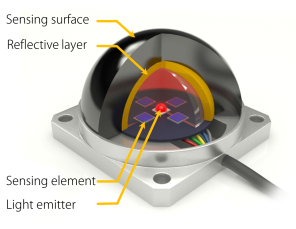
\includegraphics[scale=0.8]{Figures/OptoforceBuild}
    \caption{Figure showing construction of the 3d optical force used in thesis \cite{OptoforceFig}}
    \label{fig:OptoforceBuild}
\end{figure}
\FloatBarrier

The sensor consists of a light emitter (LED) and four sensing elements(photodiodes) which is wrapped within two layers, a reflective layer and a sensing surface. The four photodiodes will measure the force by measure the infared light reflected by the reflective layer. If a force is applied on the sensing surface, the amount of reflected light to each photodiodes will change accordingly. The forces in x- and y-direction is measured from the difference in amount of reflected light between the two opposing photodiodes for each direction, while the force in z-direction is the average of the four measurements. Which direction x, y and z-direction is shown in figure \ref{fig:OptoforceAxis}. Optoforce sensor is relative new sensor(2015), and the manufacturer claim the sensor can guarantee precise measurements even up to 200\% overload \cite{Optoforce2}. A several work where the sensor is used can be found in \cite{7803326,7759112,7849467}.


\begin{figure}[h]
    \centering
    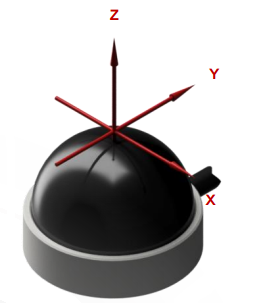
\includegraphics[scale=0.8]{Figures/OptoforceAxis3}
    \caption{Figure showing the x,y and z-direction for the 3d optical force used in this thesis \cite{OptoforceSheet}.}
    \label{fig:OptoforceAxis}
\end{figure}

\section {Machine learning}
Machine learning is a type of artificial intelligence where it can learn to adapt or predict from earlier dataset without being explicitly programmed. Each dataset consists of an feature vector, with an class for each dataset as output. The training process consists of analyzing the each features vector and produce an inferred function, which can be used for comparing new and unseen dataset to a class. The learning algorithm can be separated into supervised, unsupervised, reinforcement learning, evolutionary learning. Supervised learning is most common used within terrain classification, while few unsupervised learning. In this project will supervised learning be used. 

\paragraph{Supervised learning}
Supervised learning algorithms make predictions based on labled dataset. That is, the system know the correct answers to each dataset and make prediction based on that. The learning process usually stops when the algorithm converge towards an acceptable level of performance.

\paragraph{Unsupervised learning}
Unsupervised learning algorithms make predictions from data points without label. That is, the system has to organize the data on its own and make prediction based on that. A commom method to organize the data is by clustering.

\paragraph{Reinforcement learning}
Reinforcement leanring algorithms will gets to choose an action in response to each dataset. It will then either receieve a reward indicating how good the decision was. Based on rewards, the algortihms modifies its strategy in order to get the highest reward.

\paragraph{Evolutionary learning}
Evolutionary learning: Biological organisms adapt
to improve their survival rates and chance of having
offspring in their environment, using the idea of
fitness (how good the current solution is).



\subsection{Classifier}
The classifier is the component with the learning process and produce the inferred function. There is a vast number of classifiers and various of each classifier has been used within the terrain classification, neural network \cite{6784609,5752869,4654717}, adaptive bayesian filtering \cite{5152327,6849778}, support vector machines \cite{5602459,4161556,4059113} and decision tree \cite{6849778}. The following section will introduce technical background of five different classifiers which is intended to be used in this thesis.

\subsubsection{Neural network}
Artificial Neural Network (ANN) is a computational model based on brain, and is one of the most used learning algortihm. It can be found in many different research field, such as signal processing, image processing, control, natural language processing etc. A simple model of neuron is shown in figure \ref{fig:NN}. A neuron consists a set of weighted inputs $w_i$, an adder which sums weighted inputs signals and an activation function to decide whether the neuron should fire with an output o, for the current input, $x_i$. 
\\
\\
A single neuron will not be able to generalize the data set. However, by connecting many neurons togehter, one will obtain neural network, which is more capable to generalize data. One of the most known neural network is the perceptron. Note that neurons in the perceptron are completely independet of each other, but are dependent of all inputs and its error. That is, a neuron will not be affected by other neurons performance. Each neurons gives a result based on own weights and the input, adding them together, and comparing the result to its own threshold. The only thing neurons share is the input. 
\\
\\
The process of perceptron in supervised learning, is to learn to reproduce a particular target, which is a pattern of firing and non-firing neurons for given input. If some of the neuron got a wrong output, for instance a neuron did not fired when it should, then its weights should be adjusted to make it fire right next time. This is a single layer perceptron and good use if a problem is linearly separable. Adding more layers will make the neural network more complex and powerful. This is also called multi-layer perceptron (MLP), or multi neural network.


\begin{figure}[h]
    \centering
    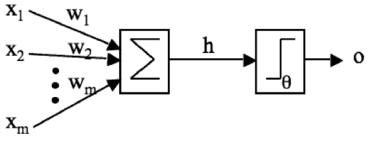
\includegraphics[scale=0.9]{Figures/neuron.PNG}
    \caption{Figure showing The three principal approaches of feature selection. The shades show the components used by the three approaches: filters, wrappers and embedded methods \cite{Guyon2006}}
    \label{fig:NN}
\end{figure}

\paragraph{Multi-Layer Perceptron}
The difference of a multi-layer perceptron and a single-layer perceptron, it that it has two or more layers between the input and output. These layer is also called hidden layer because its values are not possible to change their values directly, and only observed in the training set. The training process can be divded into two parts: forward and backwards. The forward algorithm start first by calculating the activations of the first hidden layer, and use those activations and the next set of weights to calculate the activcation of the next layer which could either be a hidden layer or the output. The output will then be compared to a target to compute an error. The backwards algorithm will be using the error to adjust the weights, firstly, between the output-layer to the hidden-layer, and the error in the hidden layer will be computed. The backwards algorithm stops when it has reach the inputs changed all their weights.


\begin{figure}[h]
    \centering
    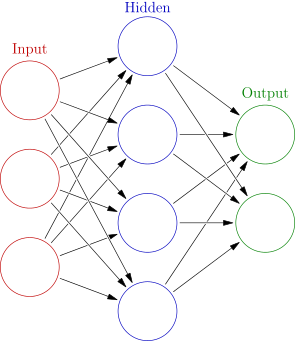
\includegraphics[scale=0.6]{Figures/MLP.png}
    \caption{Figure showing a multi-layer perceptron with 1 hidden layer \cite{MLP}. It is possible to increase the number of hidden layers and nodes to each layer}
    \label{fig:MLP}
\end{figure}

\subsubsection{SVM}
SVM algorithm was introduced by Vapnik and Chervonekis in 1963, while the standard used today is introduced by Cortes and Vapnik in 1995 \cite{Cortes1995}. In figure \ref{fig:SVM} is an instance of 2-class classification, SVM. The dotted line is the boundary for the two classes: circle and cross. To predict new set of data, it will check which side of the decision boundary it lies. If a dataset lies under the bouandary line (dotted line) it will classify it as cross and circle if above. If the decision boundary was moved small amount, there is it has a high risk of misclassifying the dataset which lie close to it. This is why SVM will find the the optimal separating hyperplan. It will classifies training data more correctly, and will also generalize better with new unseen data. To find the best decision boundary will be the maximizing the margin. It will be found by find the furthest hyperplane from a data point. If a dataset is non-linearly separable data, the SVM will transform the data into higher dimensional where the data is linearly sepearable to make the classification.


\begin{figure}[h]
    \centering
%    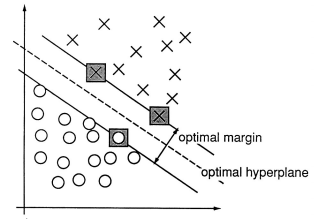
\includegraphics[width=\textwidth,height=\textheight,keepaspectratio]{Figures/SVM.PNG}
    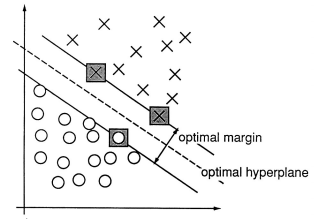
\includegraphics{Figures/SVM.PNG}
    \caption{Figure showing an example of the optimal margin for a two dimensional
two-class classification problem \cite{Cortes1995}. Each of features vector with values according to the x- and y-axis, represents as classes: circles and crosses. The 
vectors with values according to the x- and y-axis. The support vectors are the hatced classes which lies on the straight line. "The dotted line is the decision boundary/hyperplane created by the SVM".}
    \label{fig:SVM}
\end{figure}



\subsubsection{Naive bayes}
Naive Bayes algorithm is based on Bayes’ theorem the assumption of independence between every pair of features, hence the name “naive”. Bayes's theorem in machine learning is often to used to find the probability that a data set A occur, based on the data set B. Several research based the terrain classification on naive bayes which has given good result \cite{6225128, 5981563}. The bayes' theorem suit to mathematical express the terrain identification problem \cite{Giguere06environmentidentification,6225128}. This is mathematically simple and allow to evaluate unexpected mismatch between sample classes and the real environments. The terrain classification problem can be expressed as \cite{6225128}:

\begin{equation}
    P(\theta_{l}\vert X)={p(X\vert \theta_{l})P(\theta_{l})\over p(X)}
    \label{eq:bayesNaivews}
\end{equation}

The $\theta_{l}$ represent the class, which would be the possible terrains the robot is expected to predict. The X represent the observations, which are information from different sensors, also called feature vector. On the formula the \ref{eq:bayesNaivews} $P(\theta_{l}\vert X)$ is the conditional probability distribution. $P(X\vert \theta_{l})$ is the likelihood that the terrain is has with these observations, and the $P(\theta_{l})$ is the priori distribution of the classes, and $p(x)$ is the
distribution of the observation. Classification is done by selecting a class that maximizes the a posteriori probability $P(\theta_{l}\vert X)$ according to the Maximization of A Posteriori (MAP) decision rule

\begin{equation}
    p(X\vert \theta_{l})P(\theta_{l})=\displaystyle\mathop{\max}_{j}\{p(X\vert \theta_{j})P(\theta_{j})\}
    \label{eq:decision}
\end{equation}

The CPDF for each class can be estimated either parametrically or non-parametrically. An accurate nonparametric density is hard to estimate, especially when the number of features is high. One of the most popular parametric probability density functions is the normal distribution, which only requires an estimate of the mean $M_l$ and covariance matrix $\sum_1$ for the class $\theta_l$

\begin{equation}
p(X\vert \theta_{l}) = {1\over (2\pi)^{N/2}\vert \Sigma_{l}\vert ^{1/2}} \times{exp}\{-{1\over 2}(X-M_{l})^{T}\Sigma_{l}^{-1}(X-M_{l})\} 
    \label{eq:bayesLast}
\end{equation}


\subsubsection{K-nearest neighbors }
K-nearest neighbors (KNN) one of the simple classifiers presented by  T. M. Cover and P. E. Hart in \cite{1053964}. The classification process of new data consists of looking the k-nearest datapoints and classify the class which consist most classes. For instance if k is set to be 5, then it find the 5 nearest datapoint, and classify the the class which consist most of the 5 classes.  An example is shown \ref{fig:KNN}

\begin{figure}[h]
    \centering
    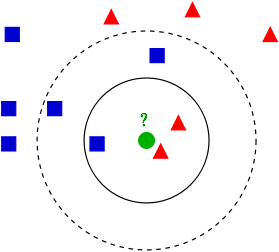
\includegraphics[scale=0.5]{Figures/KNN.png}
    \caption{Figure showing an example of a KNN\cite{KnnClassification}. All the blue squares and red triangles are the training data, while the green circle is to be classified. The straight and dashed circle illustrate which data set is taken account when k is set either 3 or 5. If k set to  3, the circle will be classified as triangle, since the tree nearest neighbor consist more triangles than squares. If k set to 5, then the cicle will be classified as square.}
    \label{fig:KNN}
\end{figure}

There are many approachs to find the k-nearest, but the most common is to calculate the Euclidean Distance. The euclidean distance can be expressed \cite{Bao2004}:


\begin{equation}
    D(x,y)=\sqrt{\sum_{i=1}^{m}(x_{i}-y_{i})^2}
    \label{eq:edistance}
\end{equation}
The Euclidean distance \ref{eq:edistance}, the x and y represent the actual and unseen class, and m is the number of features to each of classes in x and y. The algorithm will then count k classes with shortest distance to determine which class the unseen data belongs to. A weakness of using Euclidean distance function is that if one of the vector has a large range, then it will dominate other attributes. In order to avoid this issue, it is common to scale the feature, described in section \ref{subsec:scaling}


\subsubsection{Decision tree}
The decision tree is a non-parametric classifier presented by JR Quinlan \cite{Quinlan1986}. The process of the decision tree is constructing a tree consisting of nodes and edges using the dataset. Each of nodes represents a test on one features, and the edges represent an outcome of the test. Leaf nodes represent the outcome class. Predicting process is following a path from the root to a leaf node.


\begin{figure}[h]
    \centering
    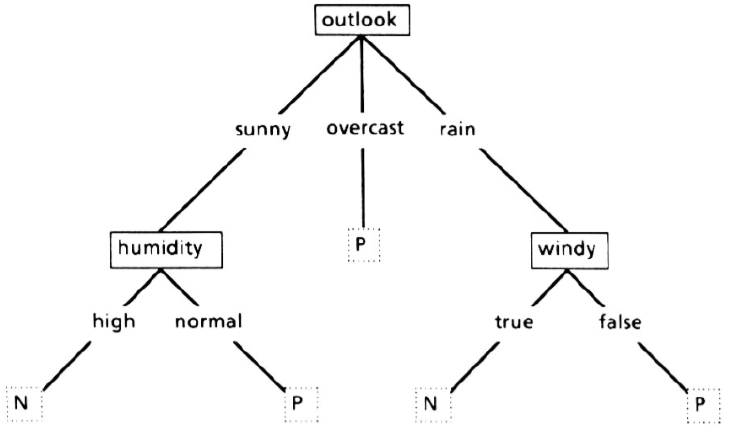
\includegraphics[scale=0.5]{Figures/decisionTree.PNG}
    \caption{Figure showing an example of a simple decision tree \cite{Quinlan1986}. This decision tree classify a day to be P or N based on outlook, humidity and windy.}
    \label{fig:SVM}
\end{figure}


\section{Features} \label{features}
An important part of good classification, is finding good features from data from sensors. The features will be used as input, to the learning, and it is the data which distinguish between the classes. Finding good features will make learning to predict more accuracy.

\subsection{Curse of dimensionality}
The curse of dimensionality occurs when one include too many features to the input vector. When the dimensionality of features vector increase, the complexity of underlying pattern might increase and the performance of the classifier will be degrade. To prevent the curse of dimensionality one can add more samples to uncover the underlying pattern.

\subsection{Features extraction} \label{feature_extraction}
Feature extraction is the process one would use techniques to build a new set of features from the original set and use it as input. The features extraced should make it easy for a classifier to distinguish between the various classes. An example of extracting good features can be seen in \cite{5602459}. Using statistic with support vector machine gave an accuracy on 40\%, while principal component analysis gave an accuracy on 78.75\%. Note that the author only used variance, kurtosis and skewness as statistic features.
\\
\\
A variety of features is used to preprocess raw sensory streams. Leaving visual feature aside, the most common is the combination of stastical moments (mean, varianc,skewness, kurtosis etc.) in the time domain with frequency domain features \cite{5152662} \cite{Giguere2009} \cite{5509309}. While others only use the frequency domain \cite{4543710} \cite{5979766}.

\subsubsection{Statistical features}
Formler\cite{Press:2007:NRE:1403886}
\paragraph{Mean}
The mean is generally referred to the average, and is defined as sum of the values divided by the number of values:

\begin{equation}
   \bar{x} = \frac{1}{N}\sum_{N-1}^{j=0}x_{j}
    \label{eq:mean}
\end{equation}


\paragraph{Variance}
Variance describe the spread between numbers in a data set. The variance can bew written as:

\begin{equation}
  Var(x_0\dotsc X_{N-1})  = \frac{1}{N}\sum_{N-1}^{j=0}(x_{j}-\bar{x})^2
    \label{eq:variance}
\end{equation}

\paragraph{Standard deviation}
Standard deviation is a measure of spread of a data set from its mean. High deviation indicate that the data points are further from the mean. This can be calculated by taking the square root from variance:

\begin{equation}
  \sigma(x_0\dotsc X_{N-1})  = \sqrt{Var(x_0\dotsc X_{N-1})}
    \label{eq:std}
\end{equation}

\paragraph{Skewness} 
Skewness describes asymmetry of a distribution. The formula is:
\begin{equation}
  Skew(x_0\dotsc X_{N-1})  =  \frac{1}{N}\sum_{N-1}^{j=0}\left [ \frac{x_j-\bar{x}}{\sigma} \right ]^3
    \label{eq:skew}
\end{equation}

The skewness can be either negative or positive depending on wheter data points are skewed to the left or to the right. If the data is skewed to the left indicate a negative skewness, while postivie skewness is when the data is skewed to the right. An illustration of both positive and negative skewness is shown in figure \ref{fig:skew}.

\begin{figure}[h]
    \centering
    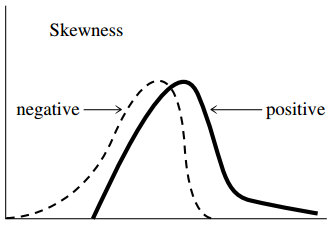
\includegraphics[scale=0.8]{Figures/Skewness}
    \caption{Skewness}
    \label{fig:skew}
\end{figure}

\FloatBarrier

\paragraph{Kurtosis}
Kurtosis measure the peak and tails of a distribution relative to a normal distribution. Using kurtosis might help to understand general characteristics about the distribution of the data. The formula is:
\begin{equation}
  Kurt(x_0\dotsc X_{N-1}) = \left \{ \frac{1}{N}\sum_{N-1}^{j=0}\left [ \frac{x_j-\bar{x}}{\sigma} \right ]^4 \right \}-3
    \label{eq:kurtosis}
\end{equation}

A positive kurtosis of a distribution has a sharper peak and heavier tails realative to normal distribution. While a negative kurtosis has flatter peak and lighter tails realative to normal distribution. An illustration of both positive and negative kurtosis is shown in figure \ref{fig:kurtosis}


\begin{figure}[h]
    \centering
    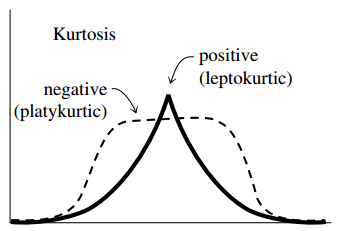
\includegraphics[scale=0.8]{Figures/Kurtosis}
    \caption{Kurtosis}
    \label{fig:kurtosis}
\end{figure}

%http://greenteapress.com/thinkstats/thinkstats.pdf

 \paragraph{Time domain}
\paragraph{Fourier transform}


\subsection{Features selection}\label{selection}
The process in feature selection is to select a subset of features from the orignial, that are relevant. Selecting good features has benefit of increasing classifier performance, reducing storage requirements and reducing training time, and defying curse of dimensionality. Note that a features can individually be completely useless can become relevant when used together with other features \cite{Guyon2006}. 
There are three types of feature selection algorithms: filter-, wrapper- and embedded methods.

\begin{figure}[h]
    \centering
    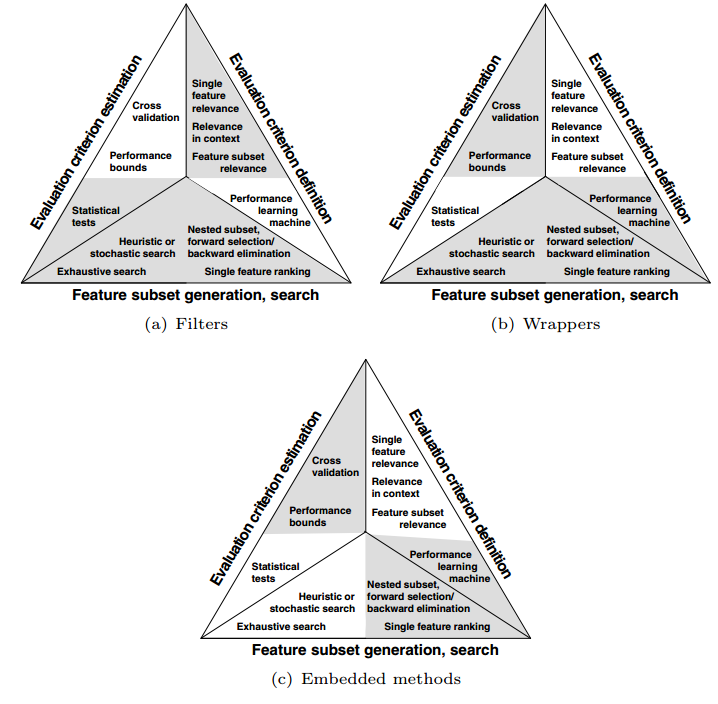
\includegraphics[scale=0.7]{Figures/FilterWrapperEmbedded.PNG}
    \caption{The figure showing the three principal approaches of feature selection. The shades show the
components used by the three approaches: filters, wrappers and embedded methods. \cite{Guyon2006}.}
    \label{fig:fitting}
\end{figure}


\paragraph{Filter}
Filter feature selection is independent of any classifier. It uses statistical measure to assign each feature a score. Feature will either be kept or removed based on the score. The filter methods are considered fast and effective, specially when the number of features is large and the number the number of available training examples comparatively small.  


\paragraph{Wrapper}
Wrapper feature selection try different combination of the feature set, evaluated by a classifier and keep the feature set with best result.


\paragraph{Embedded}
Embedded feature selection perform feature selection as part of the learning procedure and are usually specific to given classifier.

\subsection{Features scaling}
\label{subsec:scaling}
To reduce bias effect cause by skewed distributions, it is common to standardization the feature vectores. By scaling each features, it that avoid features with big number dominate compared features with small numeric ranges. It particularly affect classifier which use distance between classifier such as KNN and SVM.  By standardized feature values the features will weights equally in their representation.


\section{Model validation}

\subsection{No free lunch theorem}
The well-known no free lunch theorem\cite{NOFREELUNCH} in machine learning states that there is no best classifier for every problem. That is, even a model has a great performance for one problem, might not hold for another problem. Previous work has shown that SVM, KNN and NB gave higher accuracy than the decision tree \cite{DBLP:conf/emcr/WeissFSZ07}, while in \cite{6849778} show that NB, SVM and DT were better than KNN. It is therefore common to build several algorithms, and chose the best of them for the specified problem.

\subsection{Ovefitting and underfitting}
Overfitting and underfitting the data is a issue in machine learning which cause a poor performance of classifier. Overfitting the data occurs if there are too training data or if it has adapted to the noise in the data. While underfitting occurs if there are not enough training data and will not be able to generalize to new data. An example for each case is shown in figure \ref{fig:fitting}. The cross-validation estimate how accurately the classifier model will perform in practice, which might prevent overfitting or underfitting the data.
\begin{figure}[h]
    \centering
    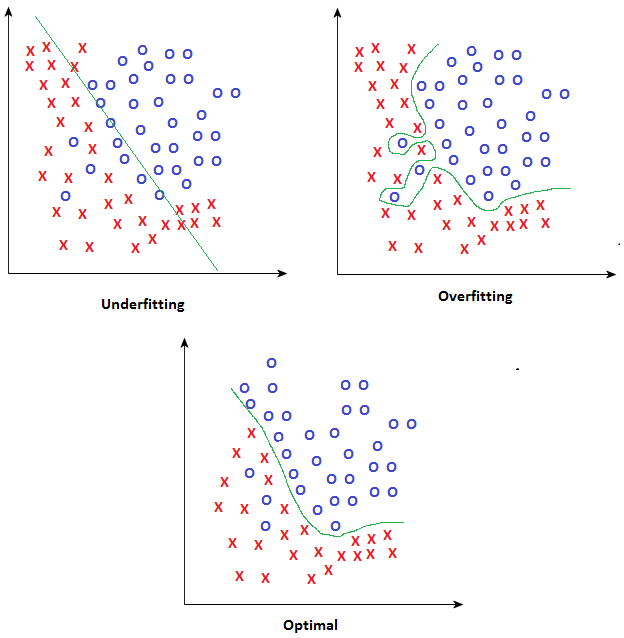
\includegraphics[scale=0.6]{Figures/All.png}
    \caption{The figure showing an example when the classifier is underfitted, overfitted or optimal.}
    \label{fig:fitting}
\end{figure}
\FloatBarrier

\subsection{Cross-Validation}
Cross-validation is used to assess the quality of a model. The process of cross-validation is to first remove some of the data before the training begins, and after the training, use the removed data to test the performance. The intention is to evaluate the classifier performance in more realistic scenario by predicting new and unseen data. There are several types of cross-validation. However the most common used in terrain classification is the k-fold cross-validation \cite{6784609,6386243,Hoffmann20141790,6849778,7387710}. 

\paragraph{K-fold}
The process of k-fold is to partitioned the data into k subset, where one subset is used for testing and the other are used for training. When the trained model has assessed the test set, a new subset is selected as test set. This process is repeated k times, that is when all subsets have been used as a test set. Setting the k to the length of feature vectors, it is also know as leave-one-outcross validation (LOOCV). LOOCV only use one feature vector as test set, while the rest as training set as shown in figure \ref{fig:kfold}. The advantages is that using as many training samples as possible.


\begin{figure}[h]
    \centering
    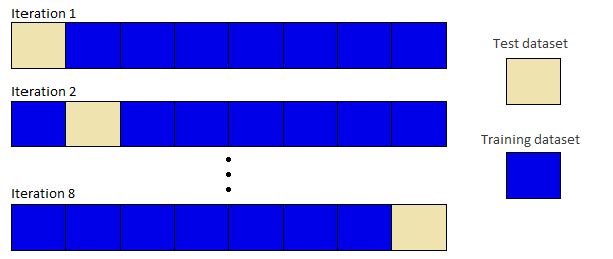
\includegraphics[scale=0.6]{Figures/Kfold}
    \caption{The figure showing an instance of k-fold cross valdiation. This is when k=n}
    \label{fig:kfold}
\end{figure}

%Se: Rigidity-based surface recognition for a domestic legged robot.


\subsection{Evaluating Classifiers}
\label{subsec:evalclf}
Evalution of the performance of the classifier can be shown by looking at the output, which could be either correct or wrong. For instance a two-class classifier with classes, "postive" and "negative" will have four different outcomes:

\begin{enumerate}
\item True postive (TP) is correct prediction of class positive
\item True negative (TN) is correct prediction of class negative
\item False positive (FP) is wrong prediction of class positive
\item False negative (FN) is wrong prediction of class positive
\end{enumerate}

Those four variables can be further used to calculate the precision, accuracy, recall and f-score.

\paragraph{Precision}
Precision gives the number of correct detected class members.
\begin{equation}
    Precision = \frac{TP}{TP + FP}
    \label{eq:prec}
\end{equation}

\paragraph{Accuracy}
Accuracy gives the ratio of correct prediction. 
\begin{equation}
    Accuracy = \frac{TP + TN}{TP + TN + FP + FN}
    \label{eq:acc}
\end{equation}

\paragraph{Recall}
Reacall gives the number of detected actual class members.

\begin{equation}
    Recall = \frac{TP}{TP + FN}
    \label{eq:recall}
\end{equation}

\paragraph{F-score}
F-score is a balanced measure of recall and precision 
\begin{equation}
    \textit{F-score} = 2*\frac{Precision*Recall}{Precision + Recall}
    \label{eq:fscore}
\end{equation}
%\part{The project}                    %% ... or ??
\FloatBarrier
It will be interesting to see which of class was easier to predict than others. This can be seen by using confusion matrix. The confusion matrix consists a square matrix with one row for predicted class, and and column for actual class (or vice-versa).
An example of confusion matrix is shown on table \ref{tab:cmatrix}

\begin{table}[h]
\centering
\begin{tabular}{ll|l|l|l|}
\cline{3-5}
 &  & \multicolumn{3}{c|}{Actual} \\ \cline{3-5} 
 &  & $C_1$ & $C_2$ & $C_3$ \\ \hline
\multicolumn{1}{|l|}{\multirow{3}{*}{Predicted}} & $C_1$ & 8 & 0 & 0 \\ \cline{2-5} 
\multicolumn{1}{|l|}{} & $C_2$ & 5 & 8 & 1 \\ \cline{2-5} 
\multicolumn{1}{|l|}{} & $C_3$ & 5 & 3 & 8 \\ \hline
\end{tabular}
\caption{A confusion matrix of 3-class classification.}
\label{tab:cmatrix}
\end{table}

\chapter{Implementation}        %% ... or ??
This chapter intends to explain the various choices which has been made to create machine learning models.


\section{Tools and environment}

\subsection{Implementation language}
The data segmentation is implemented in C++ and machine learning in python. Reading data from optical force sensor is also coded in python and taken from \cite{optoRos}. A software component framework developed for robot applications, Robot Operating System (ROS), is used to connecting each implementation as nodes. In the ROS implementation the algorithm split into several ROS nodes to allow parallell execution of the data collection and class prediction in real time whereas the python implementation runs sequentially.
\\
\\
There are many choices of programming language, but few is limited to integrate it with ROS, which are Python, C++, Lisp and MatLab. Using Java and Lua in ROS is under development. The reason of implementing data segmentation in C++ is faster Python which can deal to store and delete data stream better. Since the C++ does not has many learning library, the learning approach is implemented in Python. Python has a library called scikit-learn. It has many different type of supervised- and unsupervised learning. With all of this library it will be easy to test different classifier to find out what is the best. C++ is much faster than Python, but does not come with many learning algorithm, and it can be difficult to debug it. MatLab could also be used, it has labraries, so it would not matter whether langauge it was chosen between these two.


\paragraph{Python}
Python provide lots of libraries which provide multiple learning algorithms. The libaray's are well-documented and have the freedom to customize each algoithm to use. The library's used in this project to test different classifiers are scikit-learn, numpy, scipy and runstats.

\paragraph{Scikit-learn}
Scikit-learn is an open source library that provide tools for data mining and data analysis \cite{scikit-learn}. The library is dependent on Numpy, Scipy and matplotlib. All of classifiers, and preprocessing data tool are from this library. 

\paragraph{Runstats}
Runstats is library is used to compute statistics, such as max, mean, skew, variance and standard deviation \cite{runstats}

%\part{Conclusion}                     %% ... or Konklusjon

\subsection{Robot}
The robot used in this thesis is an Quadruped Robot developed at the University of Oslo, which is shown in figure \ref{fig:robot}. The legs are about 45 cm long and connected with optical force sensors. The OptoForce sensor is mounted on its feet. For simply set the sensor is placed in such way that it has the same direction as y-axis, which will easier to reproduce the experiments if the foot get deattach. As long one of the axis point same direction as the robot, it will be easier to reproduce experiments. Since the sensor is sensitive to x,y and z-direction, it is important that attaching both sensor in front the same way, and the for back also the same. Four different gait is made by evolutionary algorithm and is developed by Nygaard et al. \cite{7850167}. Two gaits is single-objective (SO), while the other multi-objective optimization
(MO). Only one gait is used in this project. The reason is that the other gait had issues while walking on the soft mat. The robot either got stuck (slow gait) or tipped down(fast gait). The gait is a balanced gait which let the robot go straight forward, how many steps it should walk can be done by changing a parameter in code. 


\begin{figure}[h]
    \centering
    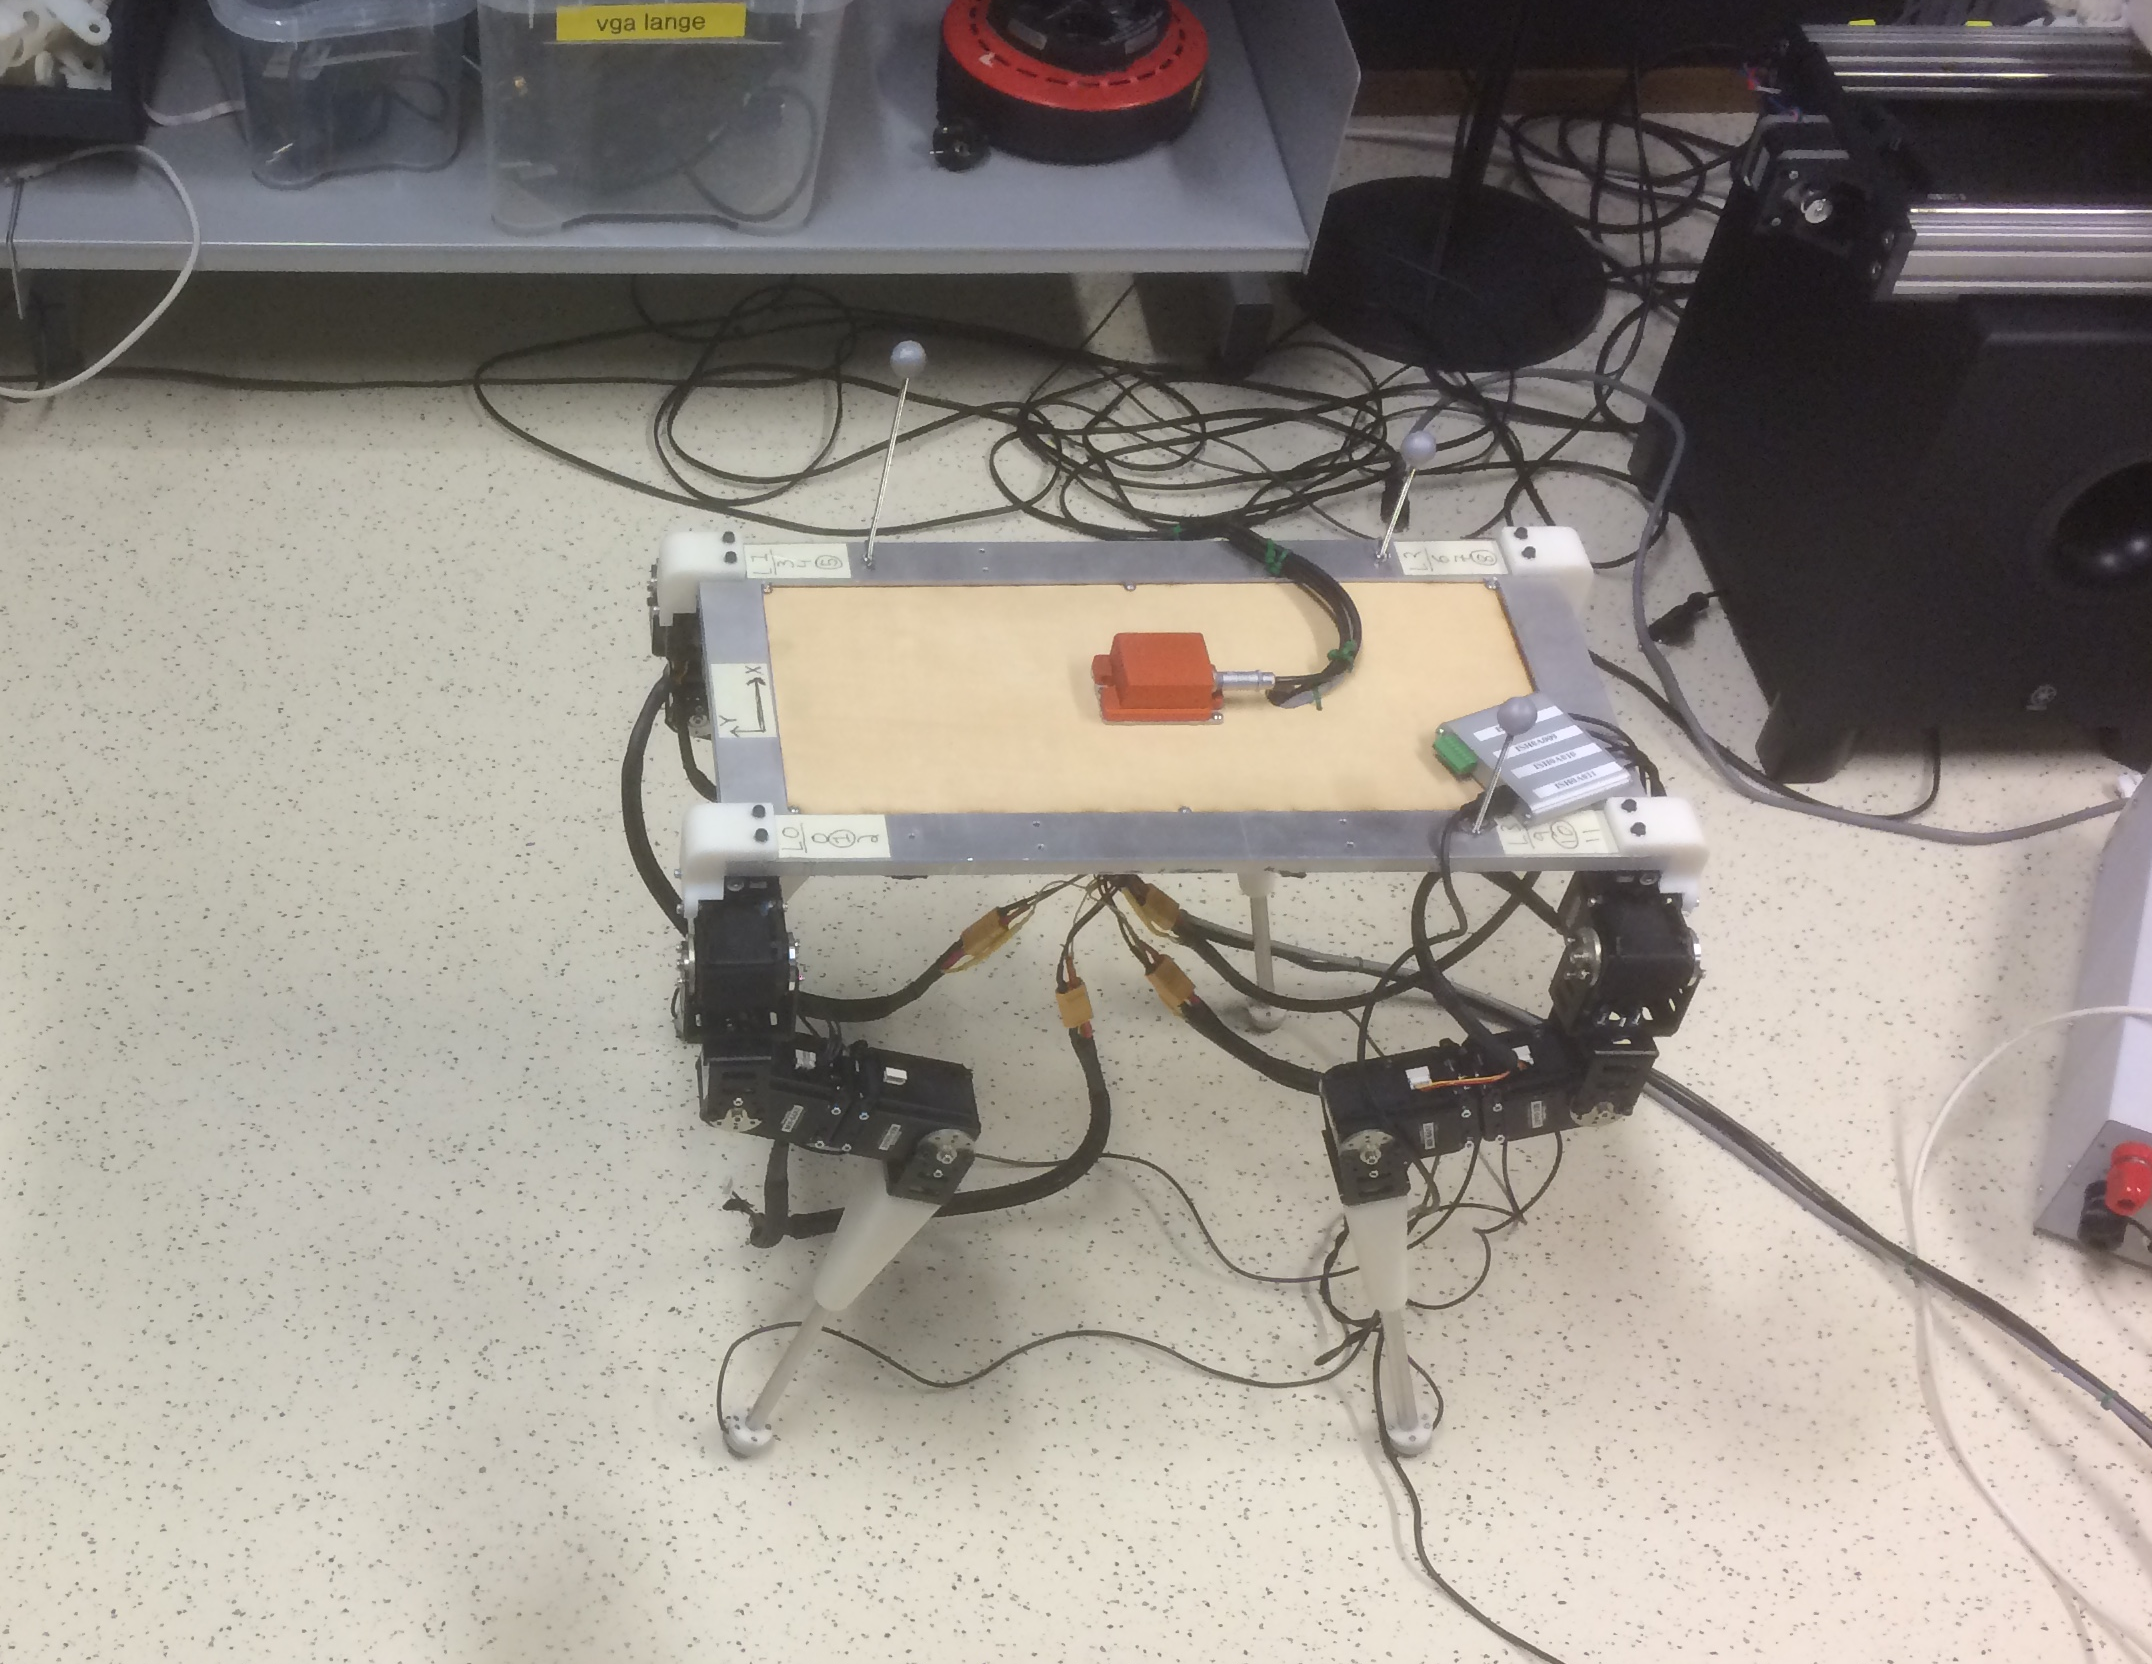
\includegraphics[width=\textwidth,height=\textheight,keepaspectratio]{Figures/Robot3}
    \caption{Figure showing the Quadruped Robot developed at the University of Oslo, which was used in all experiments}
    \label{fig:robot}
\end{figure}
\FloatBarrier

\subsection{Terrain} \label{seq:terrain}
Four different terrains will be used in all experiment, which are floor, carpet, soft mat, and hard mat, shown in figure \ref{fig:terrains}. A reason of choosing those is a more challenging task for classifier to distinguish them, cause of similarity between them. If the algorithm manage to discriminate between floor and hard mat, it might indicate that the sensor did sense some differences.  Floor, hard mat and carpet are the most difficult to distinguish, cause of similar properties. They are all slippery and has the equally hardness. Soft mat differ from the other with its softness and high friction. The experiments will be investigating whether the classifier can distinguish terrain with minor differences.

\begin{comment}
\begin{figure} 
\centering
   \begin{subfigure}[b]{0.55\textwidth}
   \includegraphics[width=1.5\linewidth]{Figures/Gulv2}
   \caption{Terrain 1: floor}
   \label{fig:Ng1} 
\end{subfigure}

\begin{subfigure}[b]{0.55\textwidth}
   \includegraphics[width=1.5\linewidth]{Figures/Teppe2}
   \caption{Terrain 2: carpet}
   \label{fig:Ng2}
\end{subfigure}
\end{figure}

\begin{figure} \ContinuedFloat
\begin{subfigure}[b]{0.55\textwidth}
   \includegraphics[width=1.5\linewidth]{Figures/Hardmatte2}
   \caption{Terrain 3: hard mat}
   \label{fig:Ng2}
\end{subfigure}

\begin{subfigure}[b]{0.55\textwidth}
   \includegraphics[width=1.5\linewidth]{Figures/MykMatte2}
   \caption{Terrain 4: soft mat}
   \label{fig:Ng2}
\end{subfigure}
 \caption{The figure showing 4 different terrains used in this project} 
\label{fig:terrains}
\end{figure}
\end{comment}


\begin{figure*}[h]
        \centering
        \begin{subfigure}[b]{0.475\textwidth}
            \centering
            \includegraphics[width=\textwidth]{Figures/Gulv2}
            \caption[Floor]%
            {{\small Floor}}    
            \label{fig:mean and std of net14}
        \end{subfigure}
        \hfill
        \begin{subfigure}[b]{0.475\textwidth}  
            \centering 
            \includegraphics[width=\textwidth]{Figures/Teppe2}
            \caption[]%
            {{\small Carpet}}    
            \label{fig:mean and std of net24}
        \end{subfigure}
        \vskip\baselineskip
        \begin{subfigure}[b]{0.475\textwidth}   
            \centering 
            \includegraphics[width=\textwidth]{Figures/MykMatte2}
            \caption[]%
            {{\small Soft mat}}    
            \label{fig:mean and std of net34}
        \end{subfigure}
        \quad
        \begin{subfigure}[b]{0.475\textwidth}   
            \centering 
            \includegraphics[width=\textwidth]{Figures/Hardmatte2}
            \caption[]%
            {{\small Hard mat}}    
            \label{fig:mean and std of net44}
        \end{subfigure}
        \caption[ ]
        {\small Four different terrain used for classification} 
        \label{fig:terrains}
    \end{figure*}

\section{Data from optical force sensor}
This section will first describe how the measurement from sensor gathered. Next, it will present how the data is segmented into sequences and used as the basis for creating feature vectors.

\subsection{Data collection}
Reading from the sensor is set to default 100Hz. A stable gait is used to walk 10 step on each terrains. The runs were recorded into rosbag, which make it possible re-simulate the run. Five runs for each terrain, and in total 20 runs were recorded. Data stream from one sensor for each run in each terrain is shown in figure \ref{fig:gtmgraf}.

\begin{comment}


\begin{figure}[h]
	\centering
	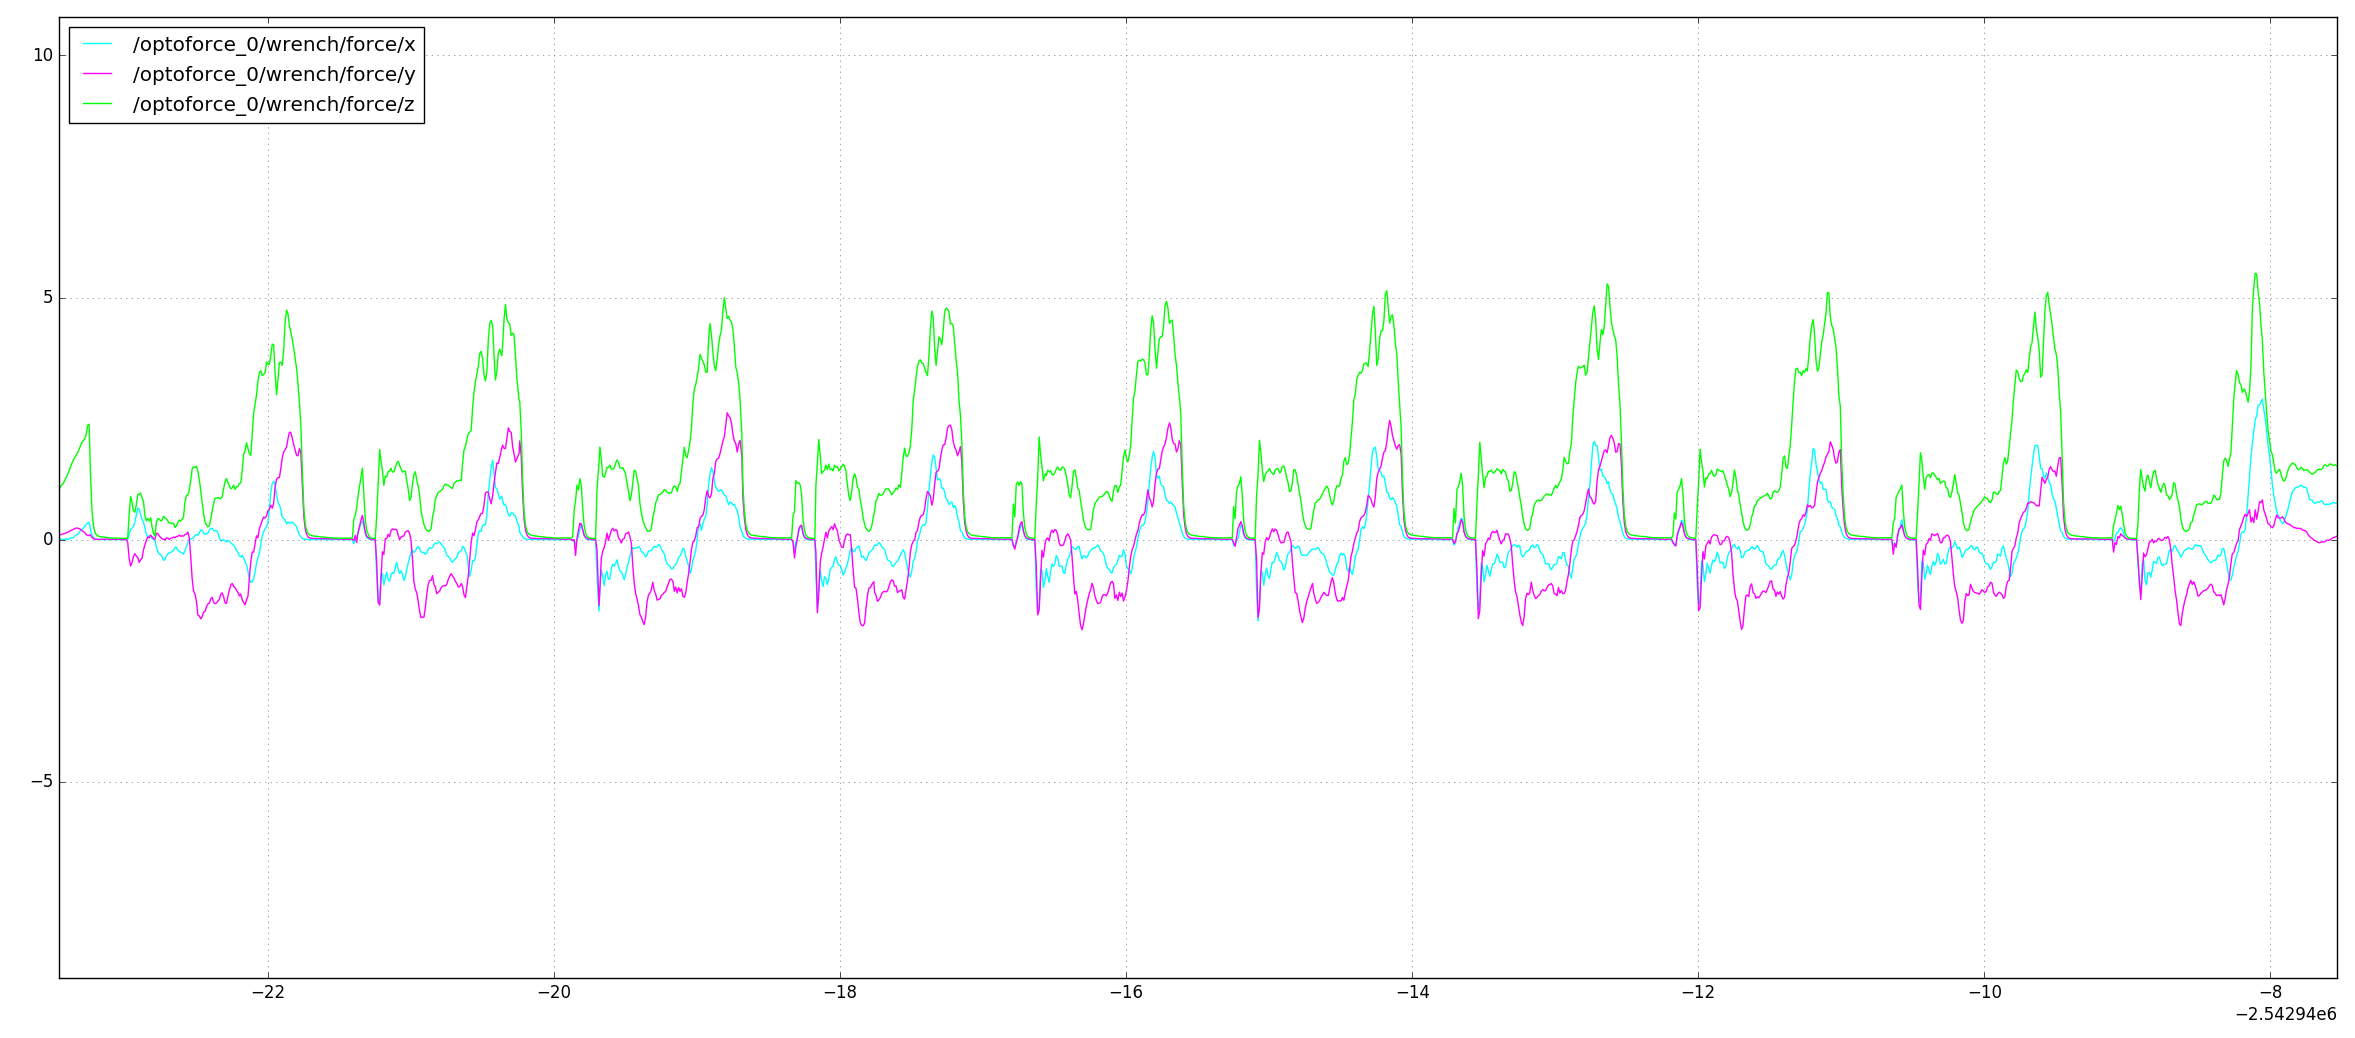
\includegraphics[width=\textwidth,height=\textheight,keepaspectratio]{Figures/gulvgraf}
	\caption{Figure showing \texttt{rqt\_plot} of a testrun on the floor.}
	\label{fig:graphf}
\end{figure}

\begin{figure}[h]
	\centering
	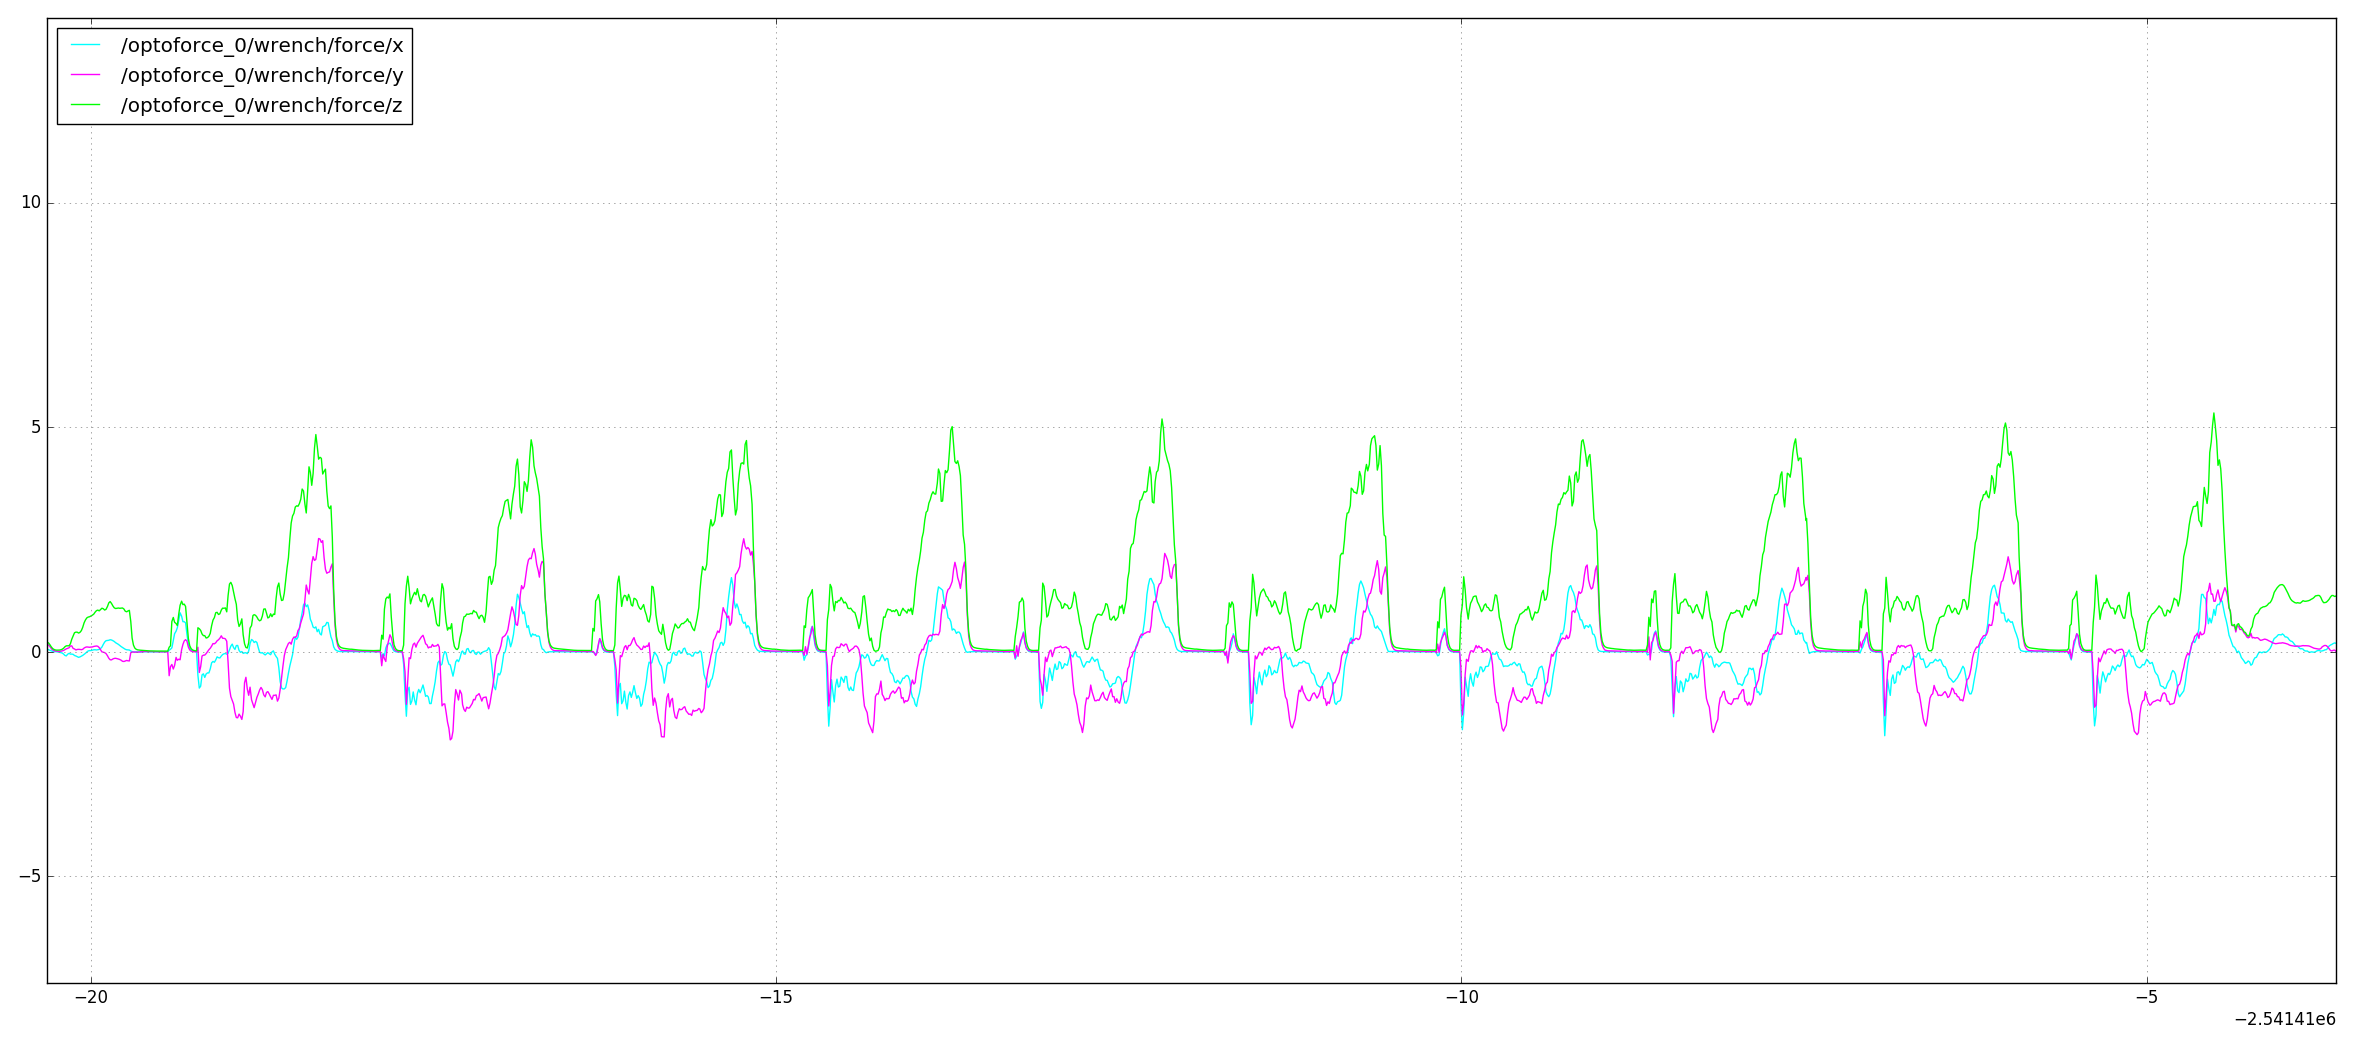
\includegraphics[width=\textwidth,height=\textheight,keepaspectratio]{Figures/teppegraf}
	\caption{Figure showing \texttt{rqt\_plot} of a testrun on the carpet terrain.}
	\label{fig:grapht}
\end{figure}

\begin{figure}[h]
	\centering
	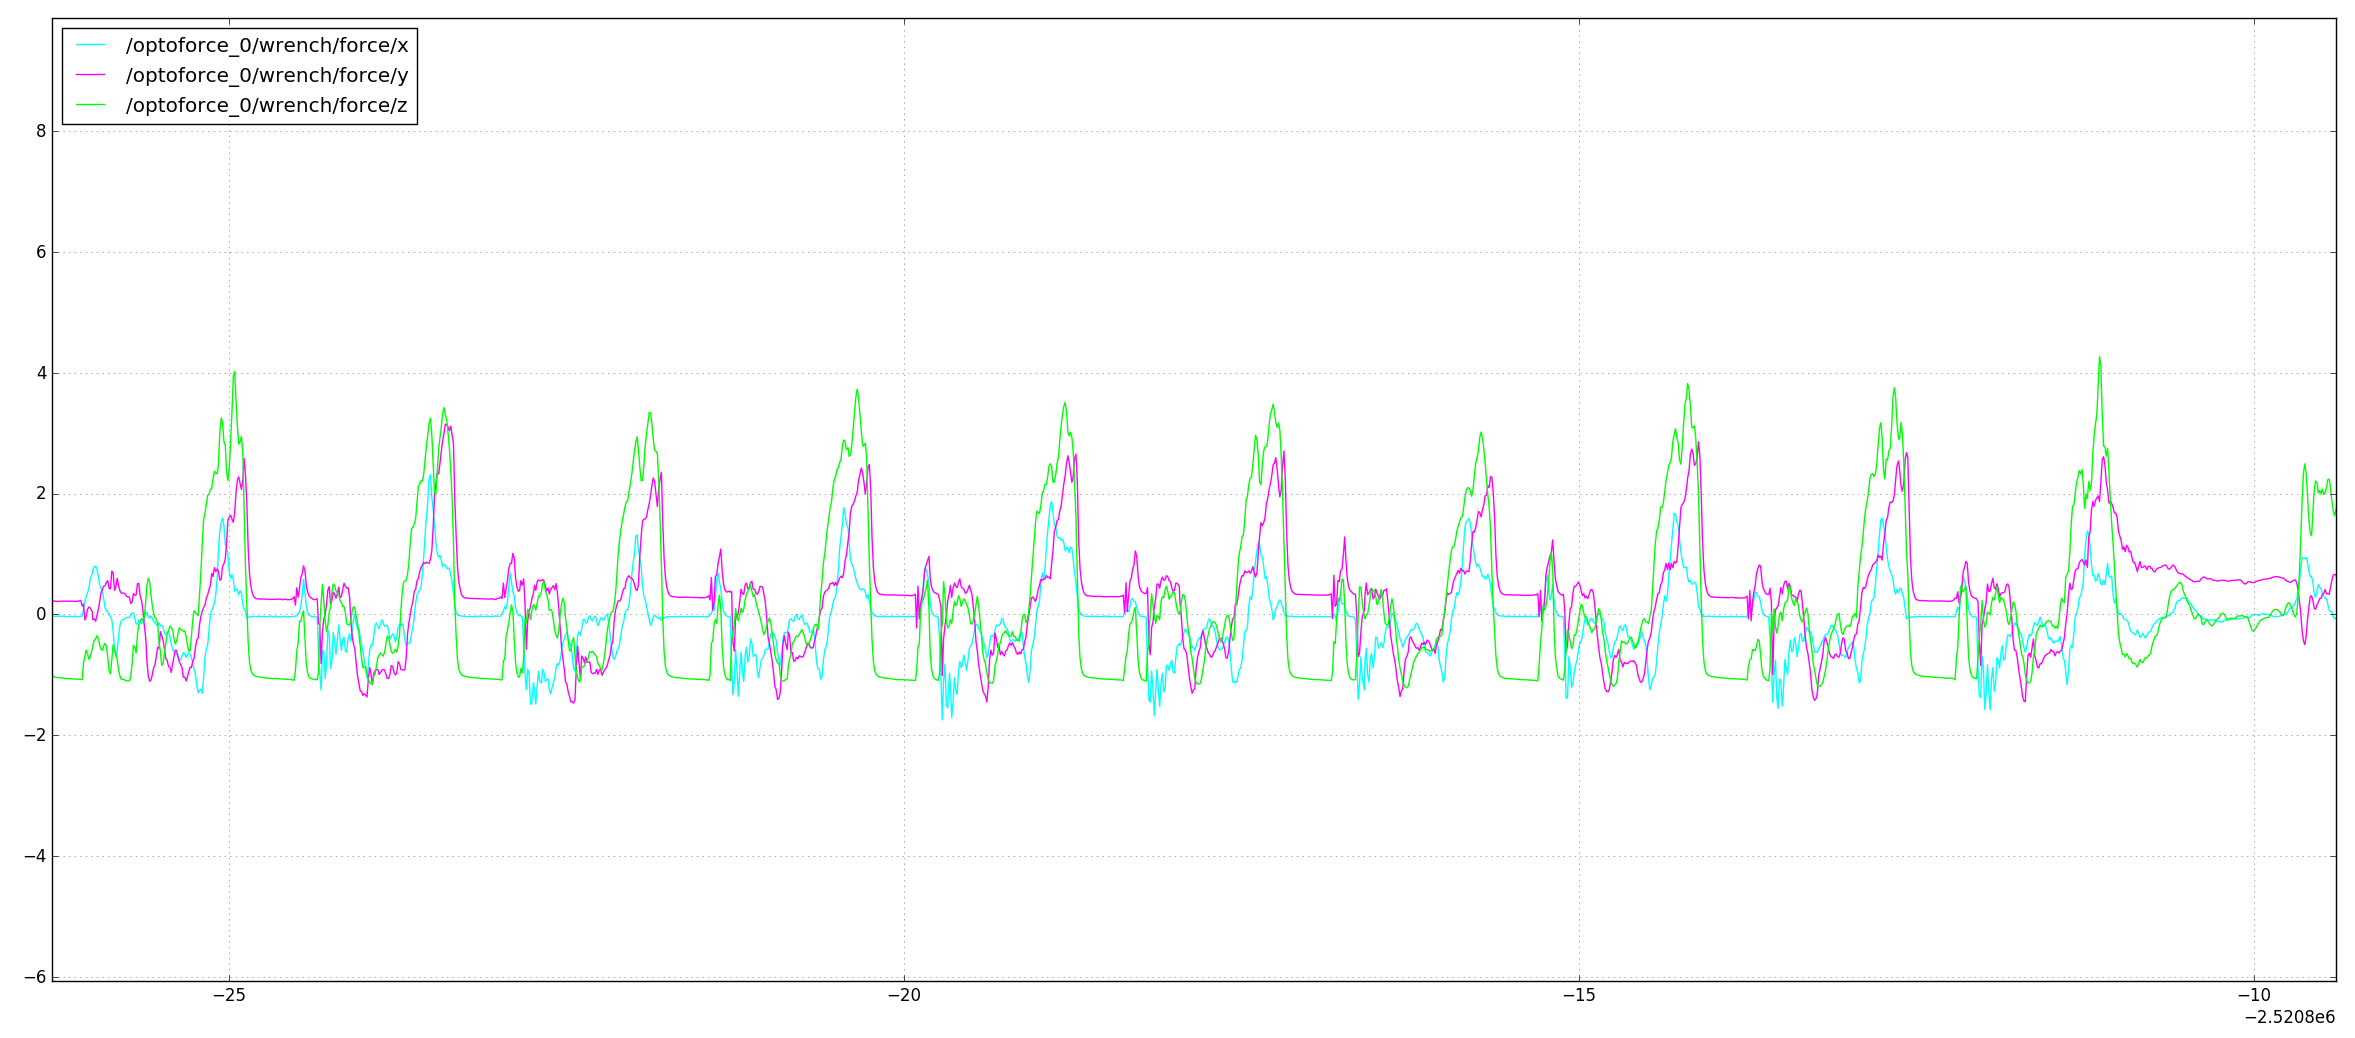
\includegraphics[width=\textwidth,height=\textheight,keepaspectratio]{Figures/mattebgraf}
	\caption{Figure showing \texttt{rqt\_plot} of a testrun on the hard mat terrain.}
	\label{fig:graphhm}
\end{figure}

\begin{figure}[h]
	\centering
	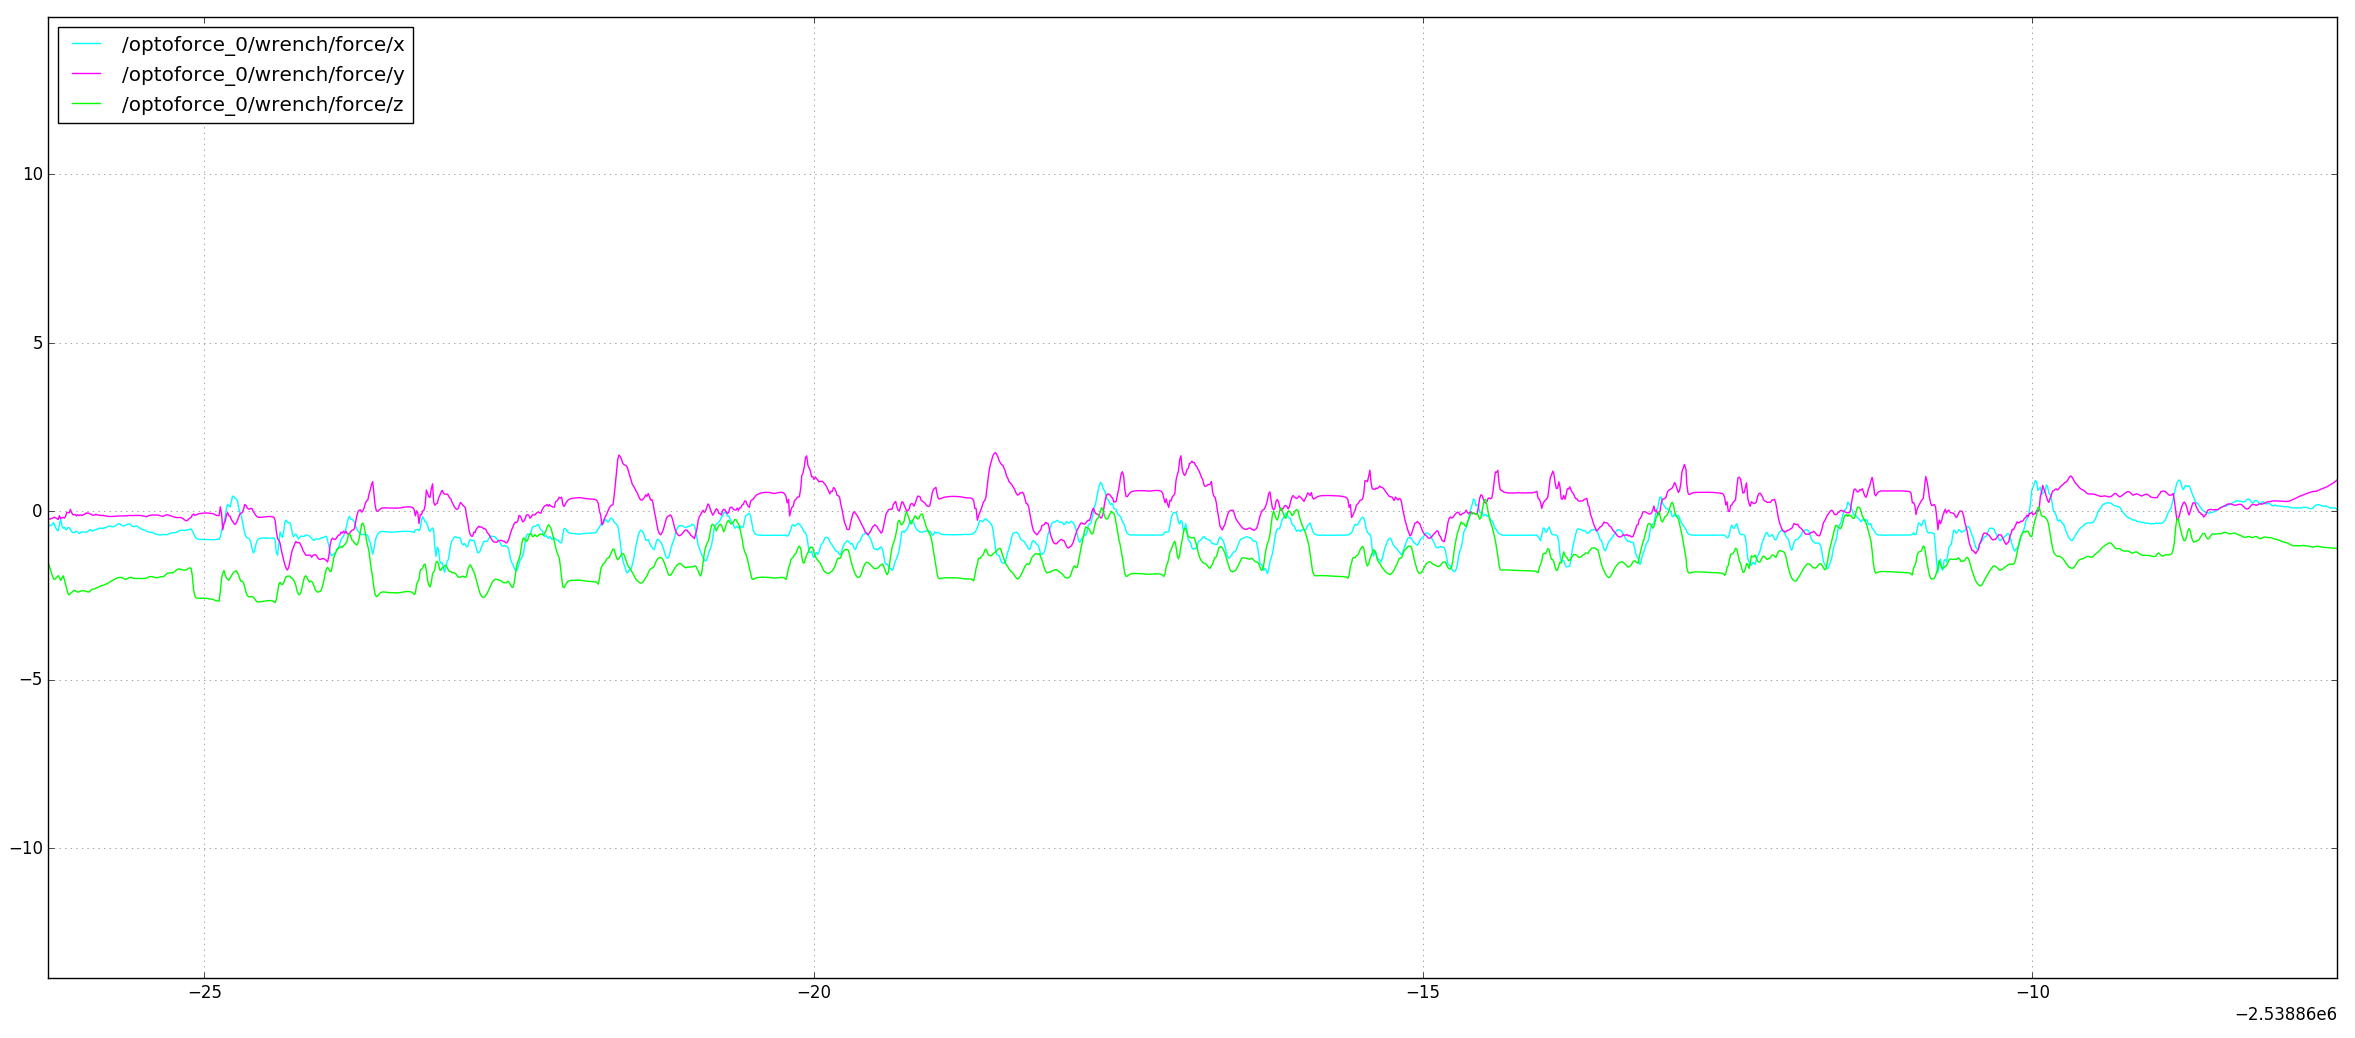
\includegraphics[width=\textwidth,height=\textheight,keepaspectratio]{Figures/mykmattegraf}
	\caption{Figure showing \texttt{rqt\_plot} of a testrun on the soft mat.}
	\label{fig:graphmm}
\end{figure}
\end{comment}

\begin{figure} [h]
	\centering
	\begin{subfigure}[b]{\textwidth}
		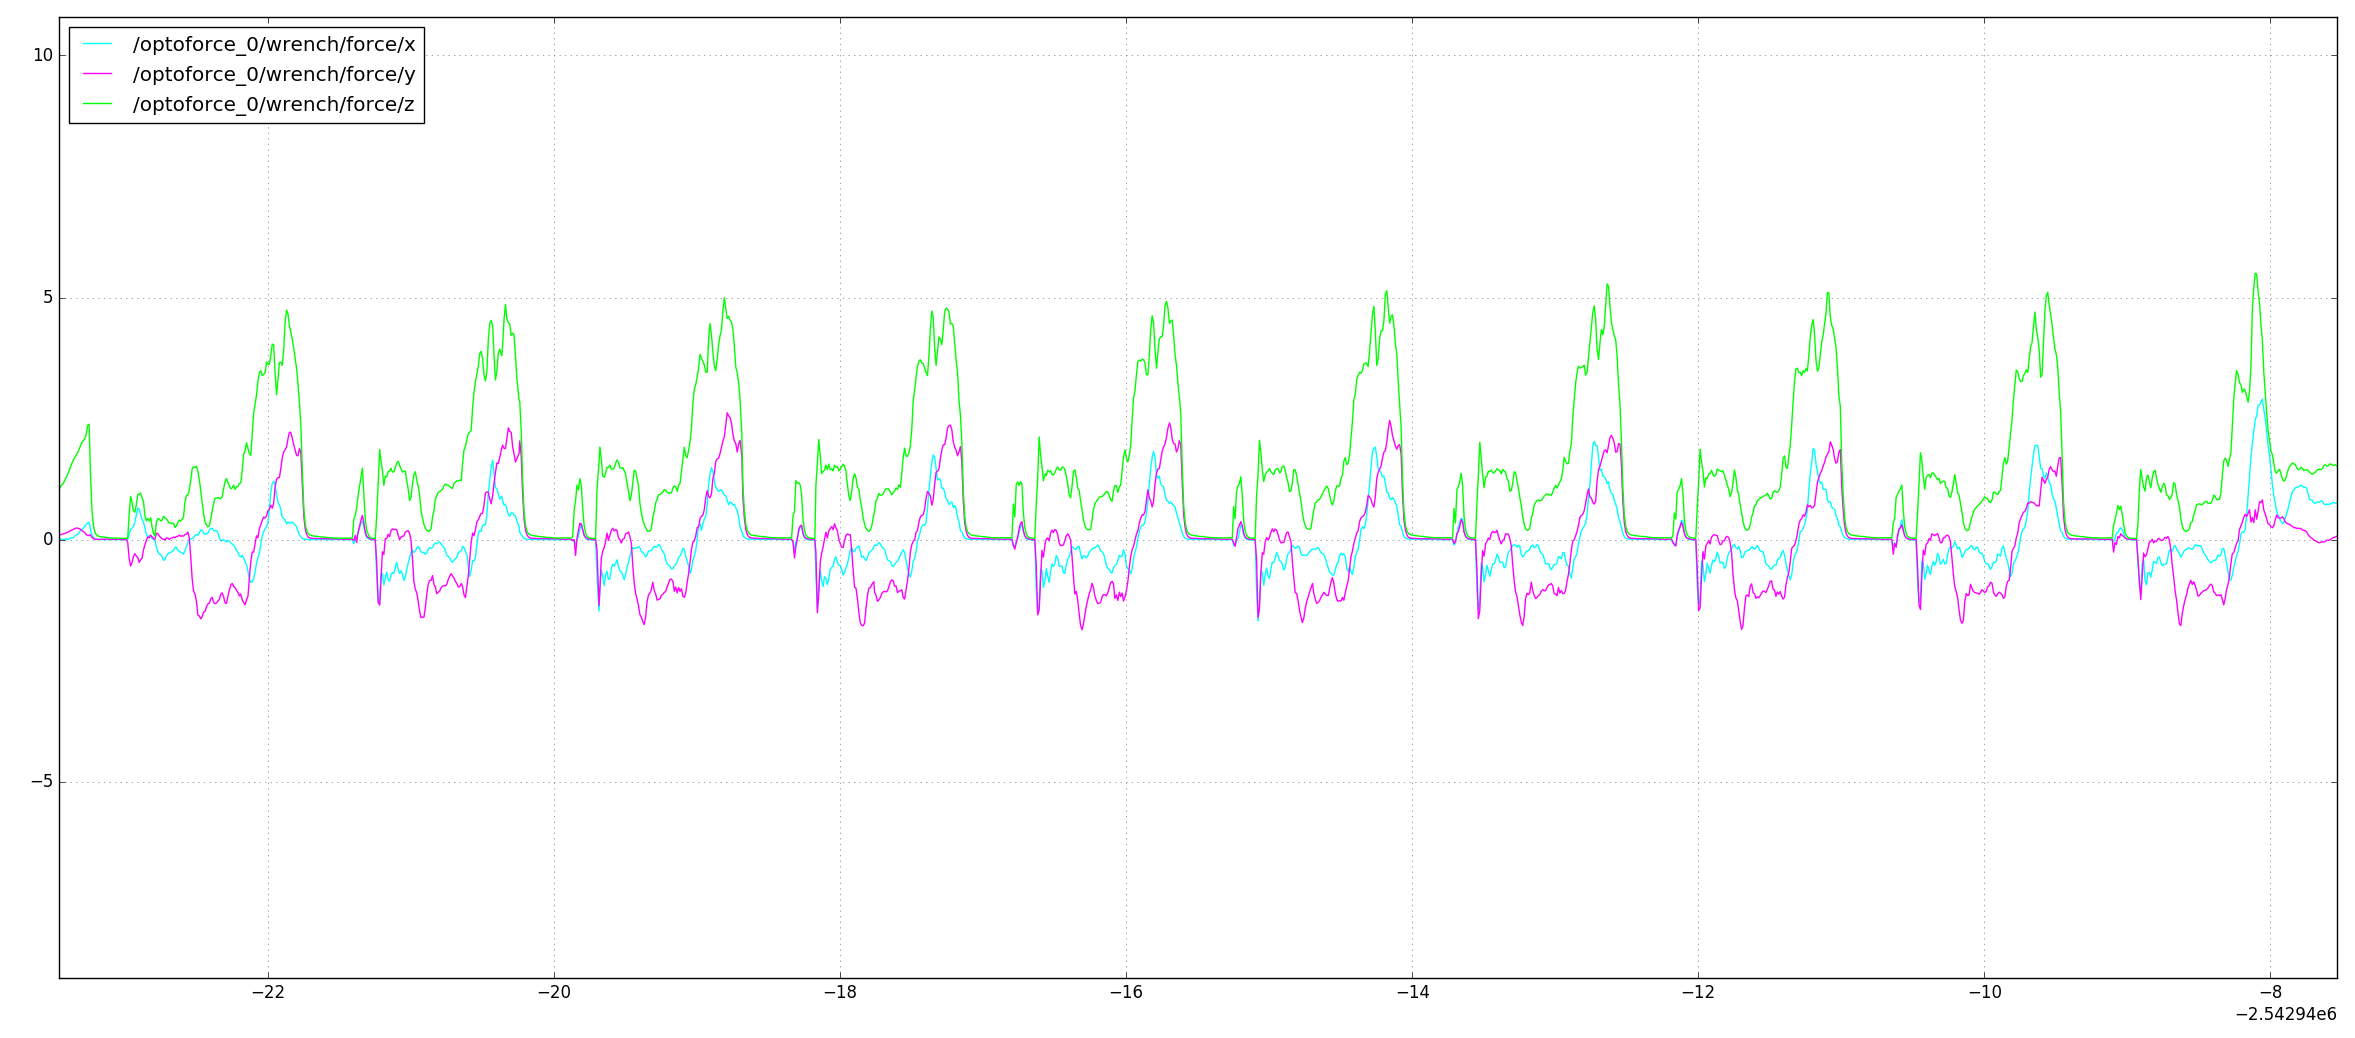
\includegraphics[width=\textwidth,height=\textheight,keepaspectratio]{Figures/gulvgraf}
		\caption{}
		\label{fig:gulvgraf} 
	\end{subfigure}
	
	\begin{subfigure}[b]{\textwidth}
			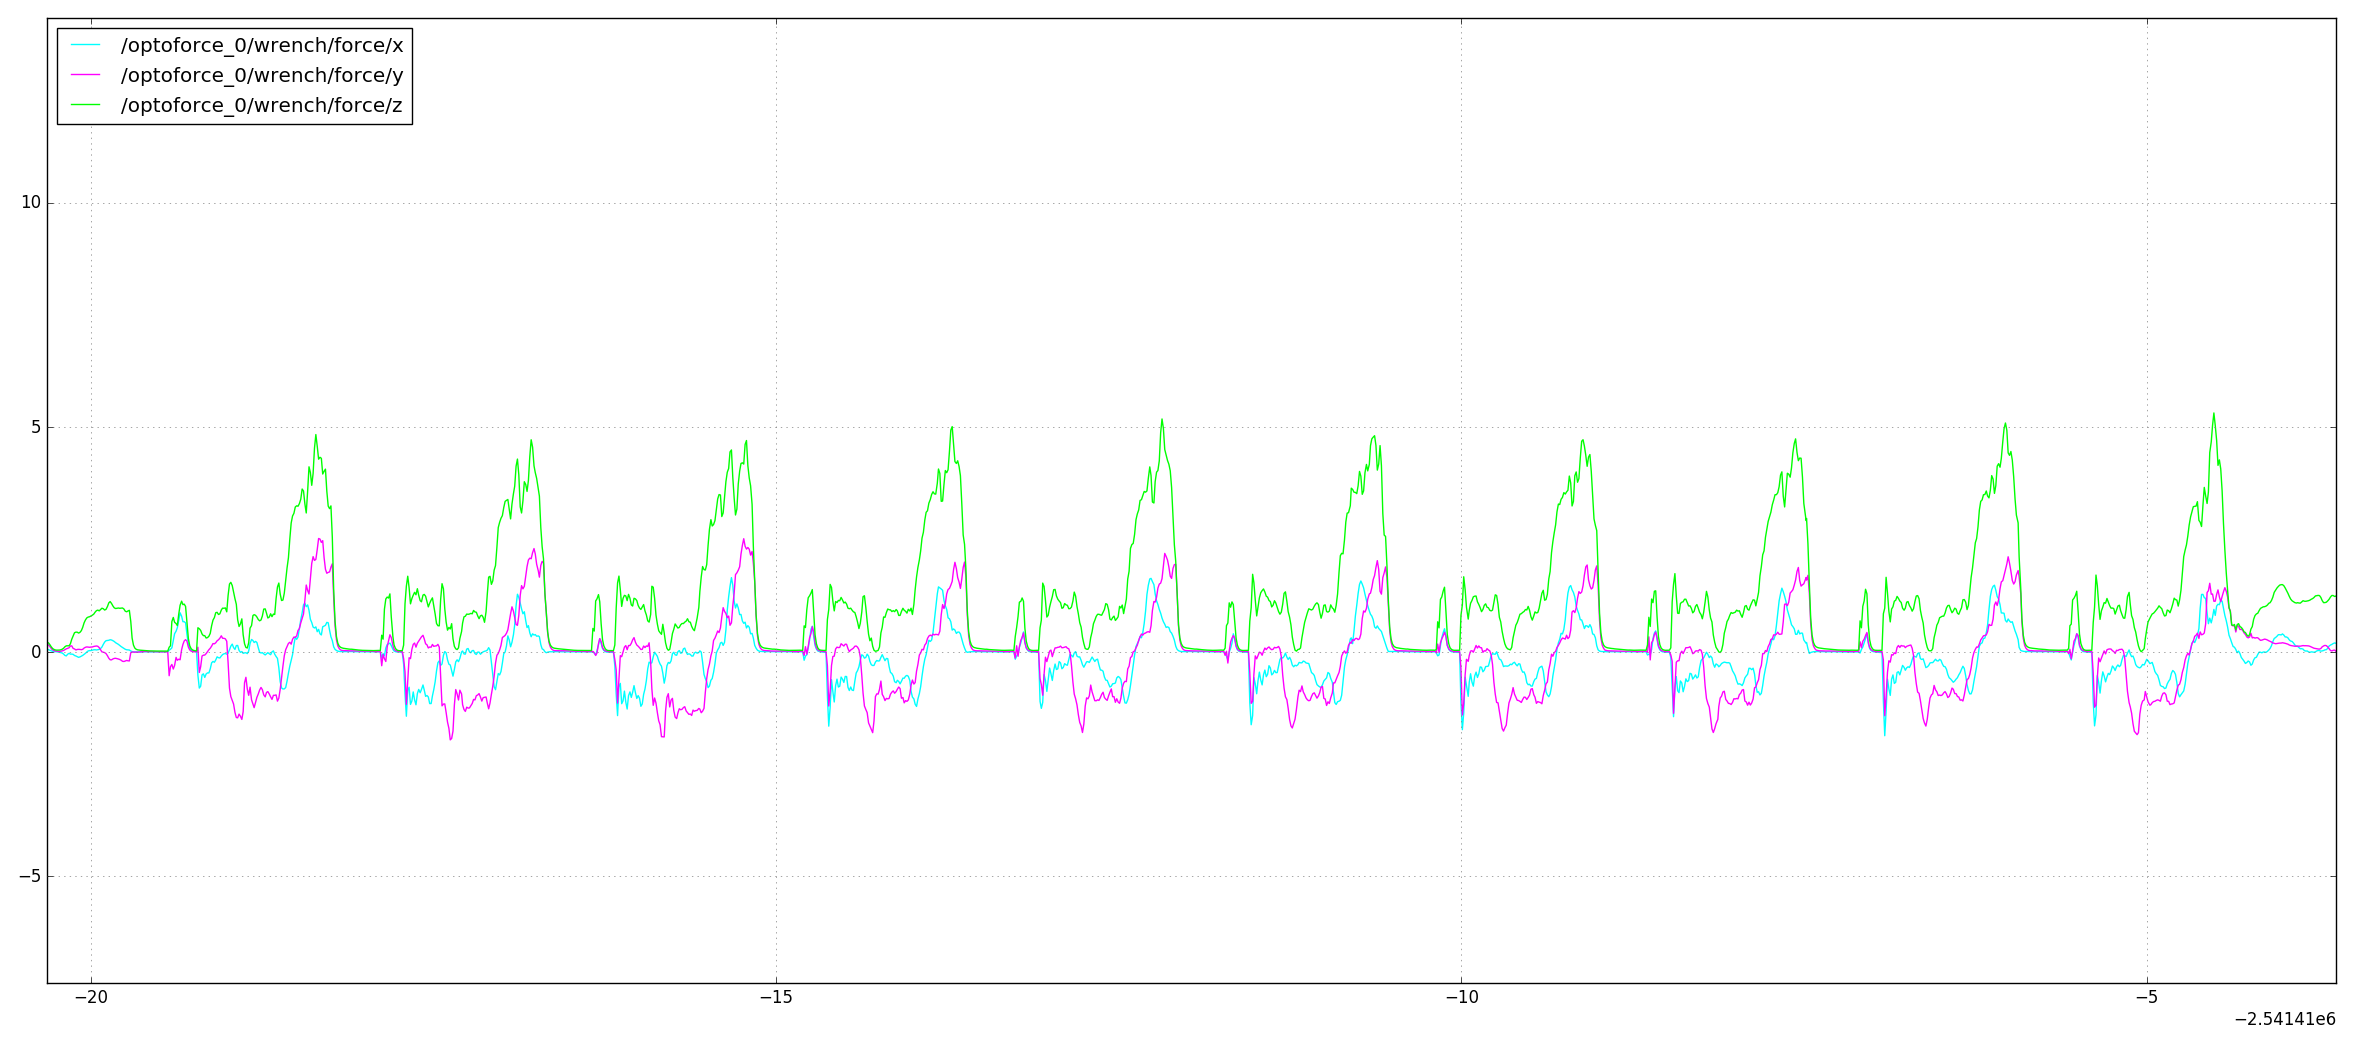
\includegraphics[width=\textwidth,height=\textheight,keepaspectratio]{Figures/teppegraf}
		\caption{}
		\label{fig:teppegraf}
	\end{subfigure}

	\begin{subfigure}[h]{\textwidth}
	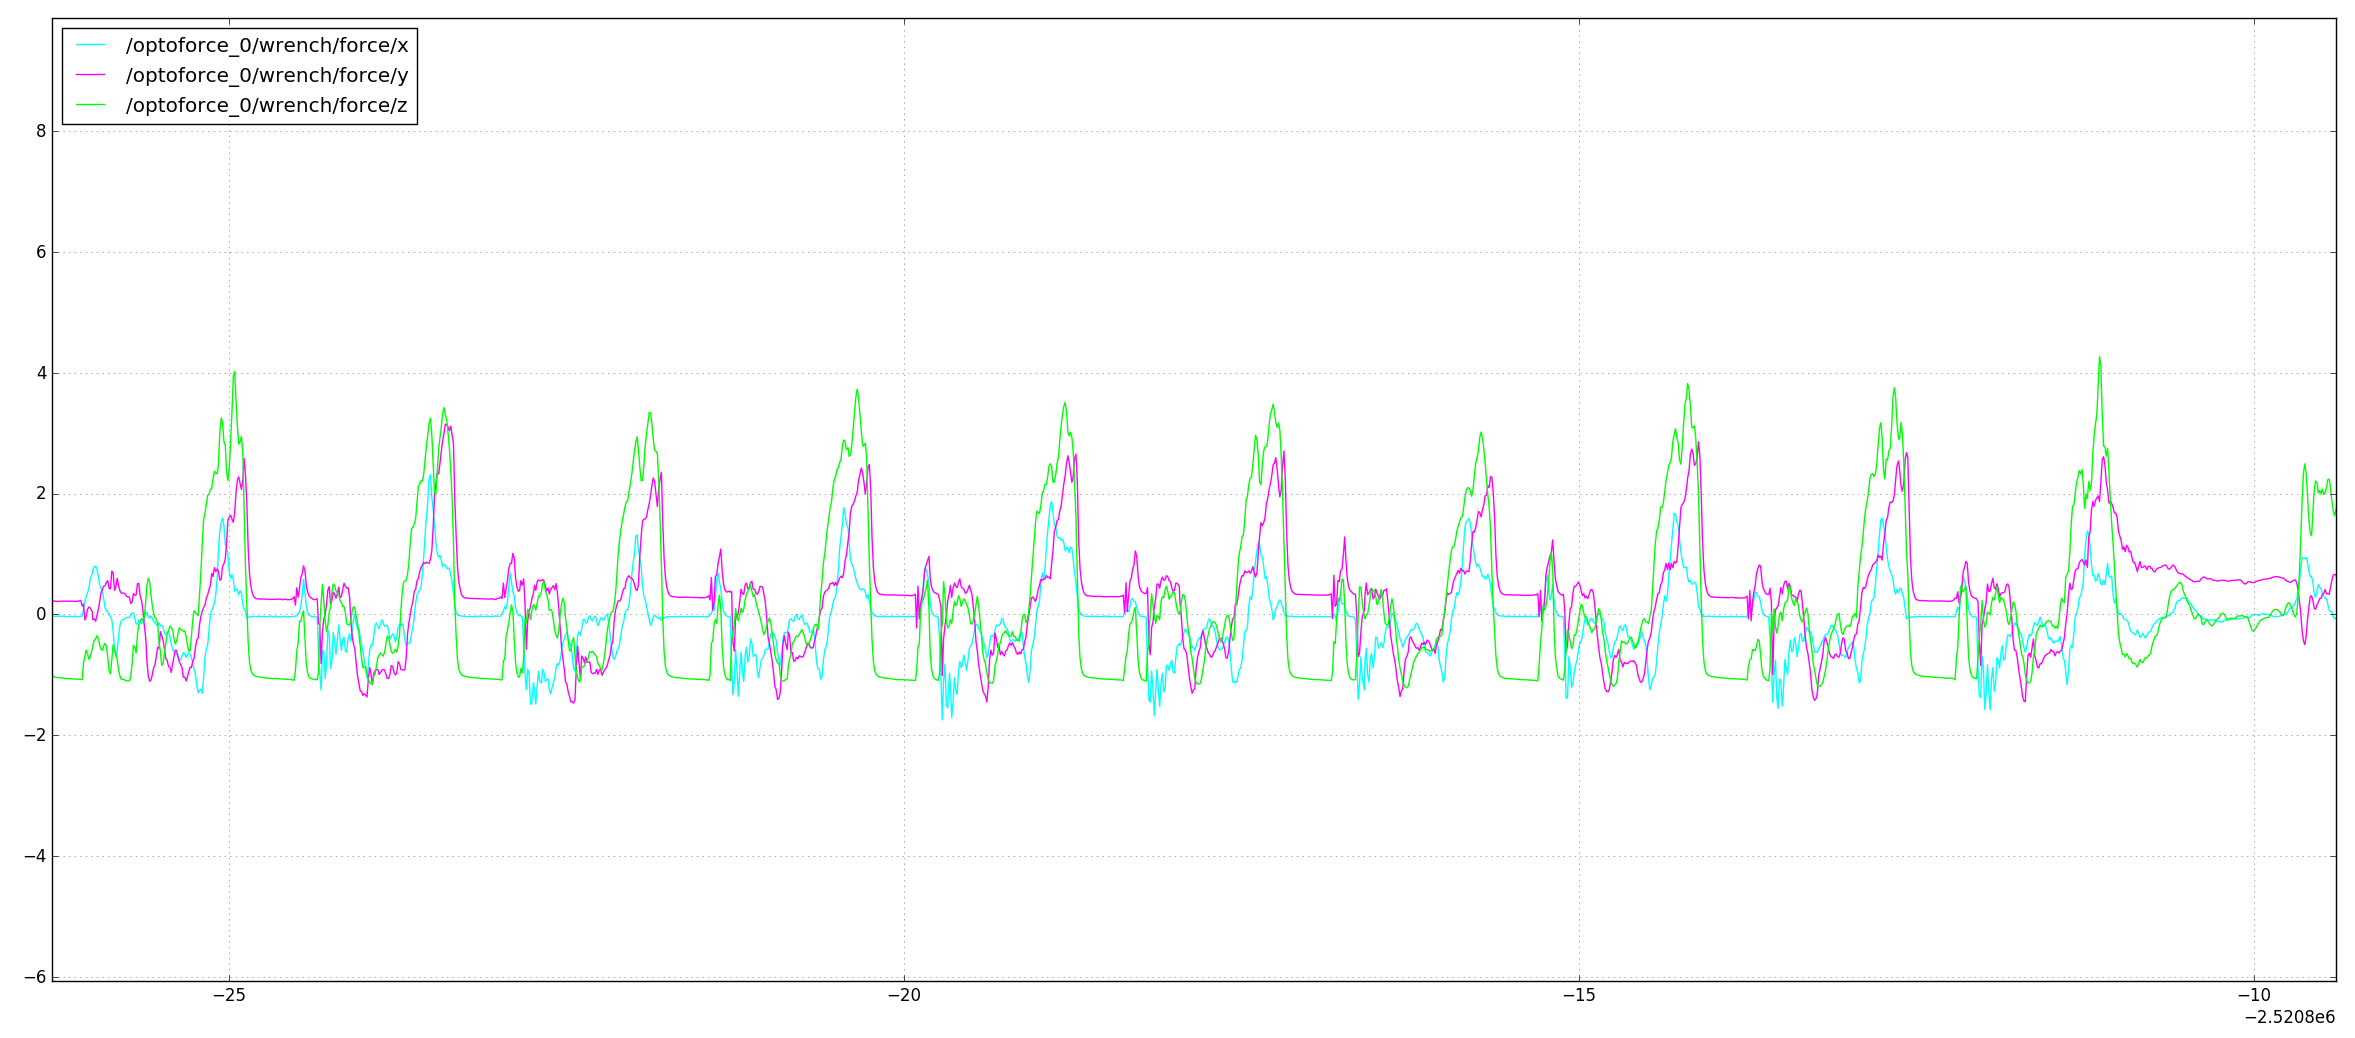
\includegraphics[width=\textwidth,height=\textheight,keepaspectratio]{Figures/mattebgraf}
	\caption{}
	\label{fig:mattebgraf}
	\end{subfigure}

\end{figure}
\begin{figure}[h] \ContinuedFloat
	\begin{subfigure}[b]{\textwidth}
			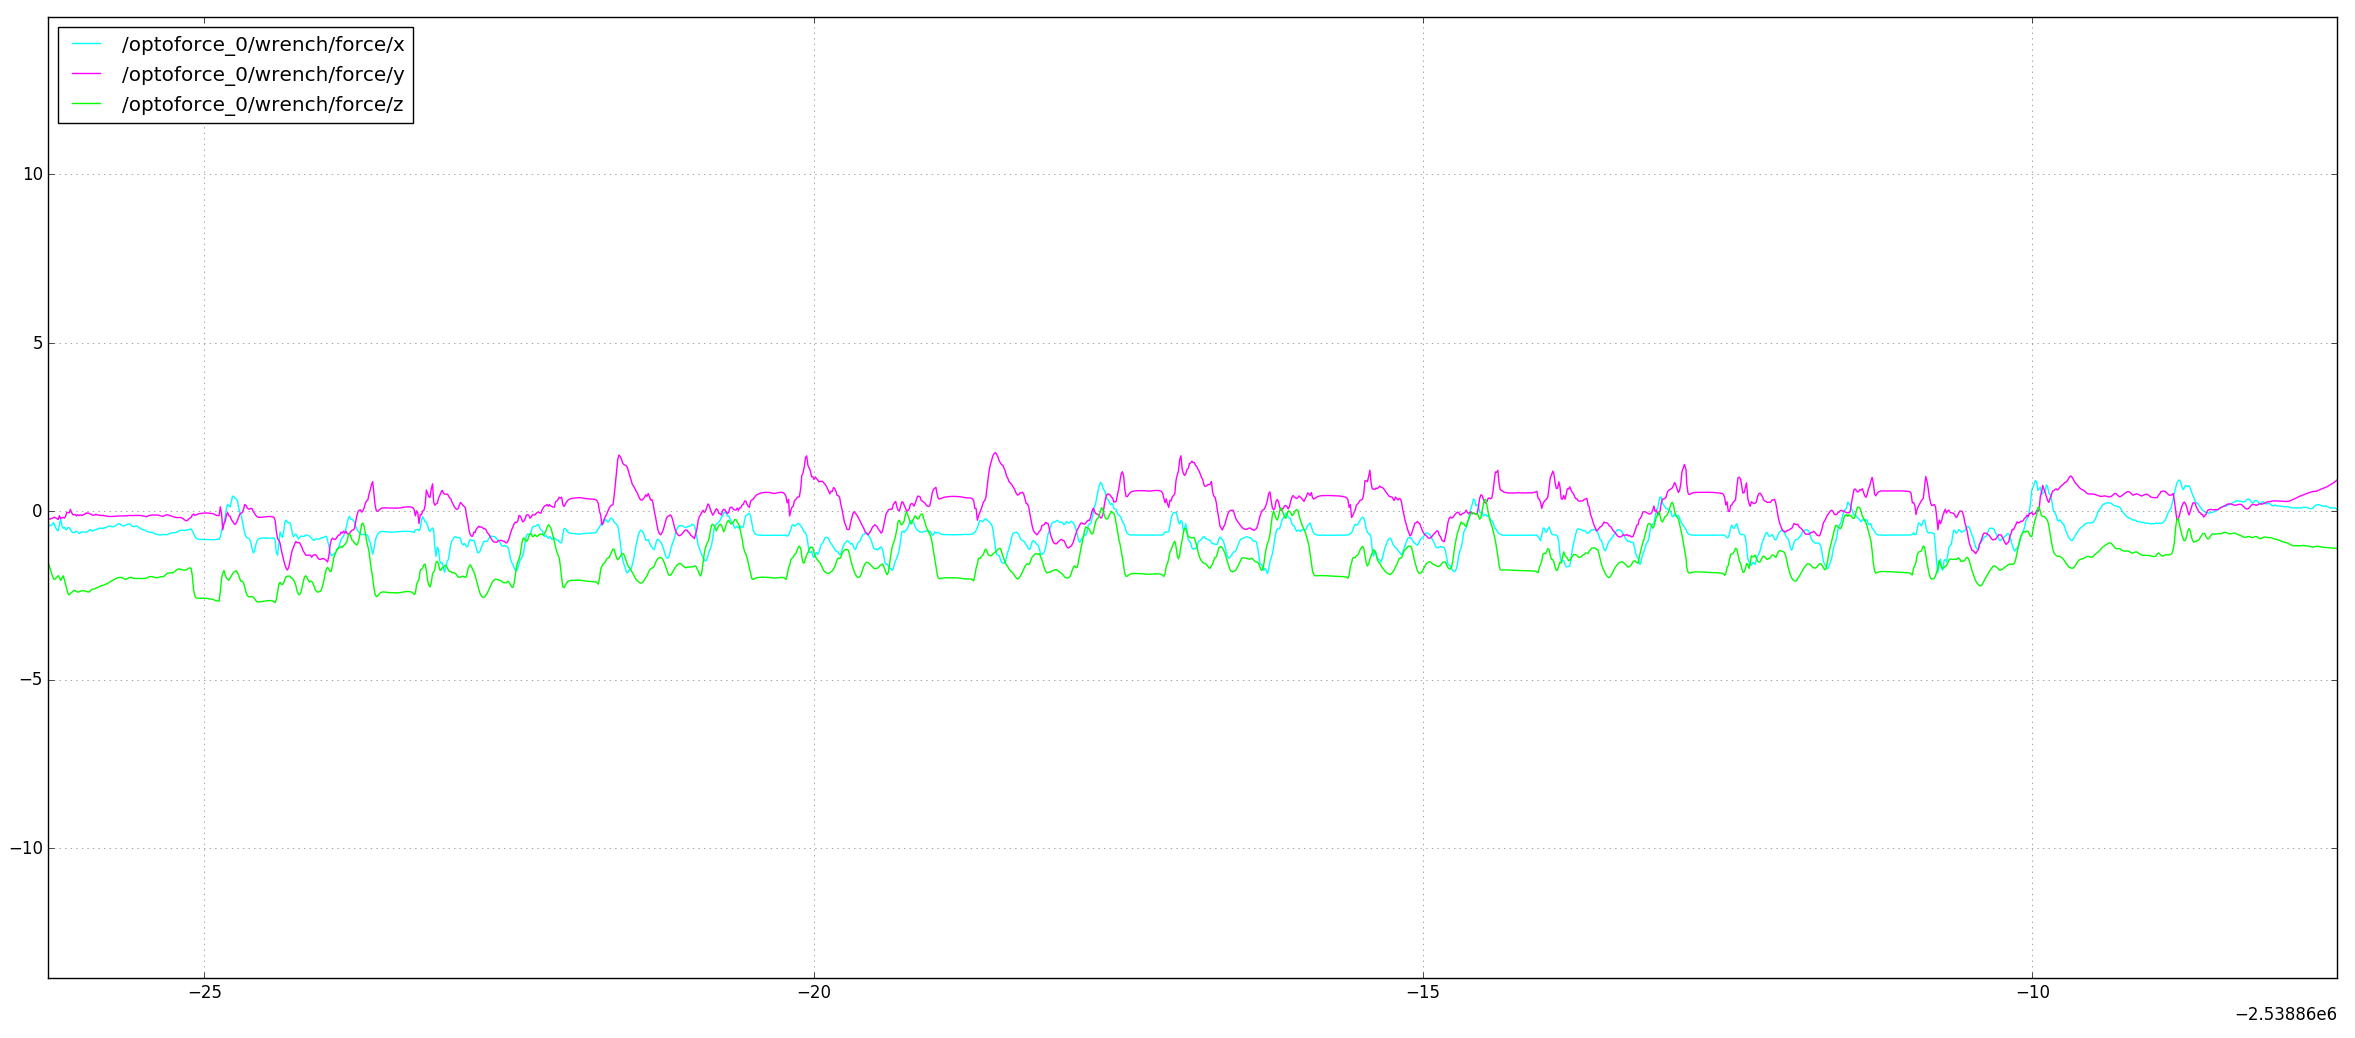
\includegraphics[width=\textwidth,height=\textheight,keepaspectratio]{Figures/mykmattegraf}
		\caption{}
		\label{fig:mykmattegraf}
	\end{subfigure}
	\caption[Two numerical solutions]{(a) Numerical solutions for the small-time system 
		with a constant-curvature body shape showing the scaled leading-order veritcal 
		reaction force $N_0$ versus the scaled body mass $M$ for various values of $g$. 
		Again, $I=M$ for definiteness and $A=0.7$. (b) As for (a) but over a wider range of 
		values of $M,I$.}
	\label{fig:gtmgraf}
\end{figure}


\FloatBarrier


\subsection{Analyzing data from sensor}
Analyzing the data is to find common characteristics and be able to segment desired data. Sensor data arrives in a stream, as shown in figure \ref{fig:gtmgraf}. The periodic sequence is for each step. A common characteristic for all terrain is when the foot is in the air, x,y, z-direction will have minor change almost constant.

\subsection{Data segmentation} \label{subseq:segmentation}
An appropriate method to segment data is sliding window algorithm. However, there are factors taken in account, which made it not to use the algorithm. It is difficult to decide an acceptable size of the window, difficulty of determining interesting data from the window and big window size is not efficient. Thus, an algorithm to segment data was created. 
\\
\\
In the thesis it is considered that the most informative from terrain is when the foot has with the ground until it is in the air. In order to collect the interested data is firstly to detect when a foot is in air. That is when there are minior change in x,y,z-direction. When there are big change in each direction, start to store the data from sensor into an array, and stop when it is in the air again. Each step will be used as a sample in training and test set. It has a restriction on when to use or not. Many runs the shortest with 125 length.


\section{Feature extraction}
As mentioned in section \ref{features}, a good classifier is depended of  good features. In the section \ref{feature_extraction} previous work have extracted features both in time domain and frequency domain. 
\\
\\
In time domain, figure \ref{fig:meanxyz} showing the mean of 10 samples in three z,y and z-direction. Carpet and Hard mat is most similar accordingly the values, which might be the most difficulty to discriminate. However, shapes of curves between floor and carpet is the most similar, which also may be not easy to predict. The soft mat differ from the other widely, and should be the easiest to predict. 
\\
\\
A mean of 10 samples in frequency domain is shown in figure \ref{fig:fftxyz}. The soft mat differ from the other widely, while floor, carpet and hard mat is similar to each other.


\begin{comment}
\begin{figure}[h]
\centering
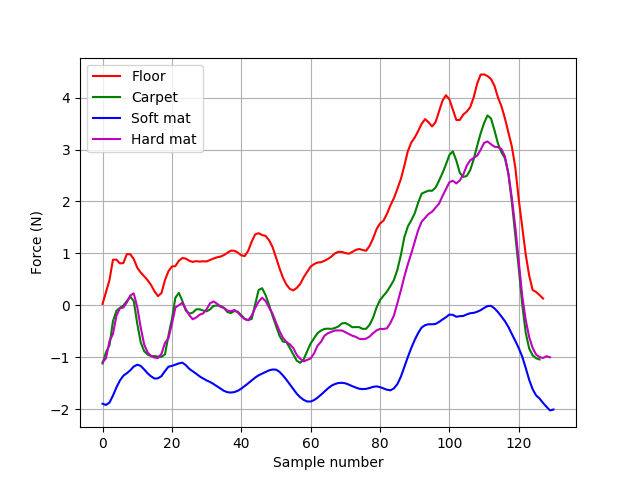
\includegraphics[width=\textwidth,height=\textheight,keepaspectratio]{Figures/meanx}
\caption{Figure showing force in the x-direction}
\label{fig:meanx2}
\end{figure}

\begin{figure}[h]
\centering
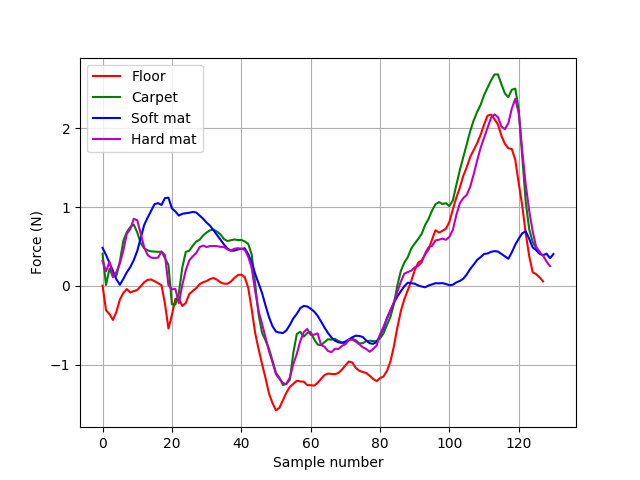
\includegraphics[width=\textwidth,height=\textheight,keepaspectratio]{Figures/meany}
\caption{Figure showing force in the y-direction}
\label{fig:optoforce}
\end{figure}

\begin{figure}[h]
\centering
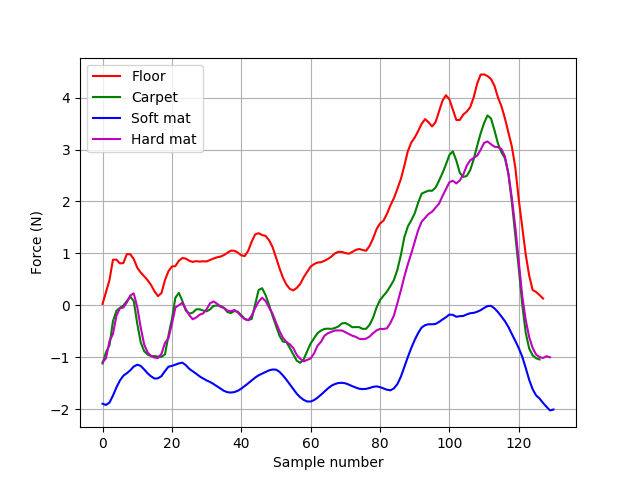
\includegraphics[width=\textwidth,height=\textheight,keepaspectratio]{Figures/meanz}
\caption{Figure showing force in the z-direction}
\label{fig:optoforce}
\end{figure}
\end{comment}

\begin{figure} [h]
	\centering
	\begin{subfigure}[b]{0.95\textwidth}
		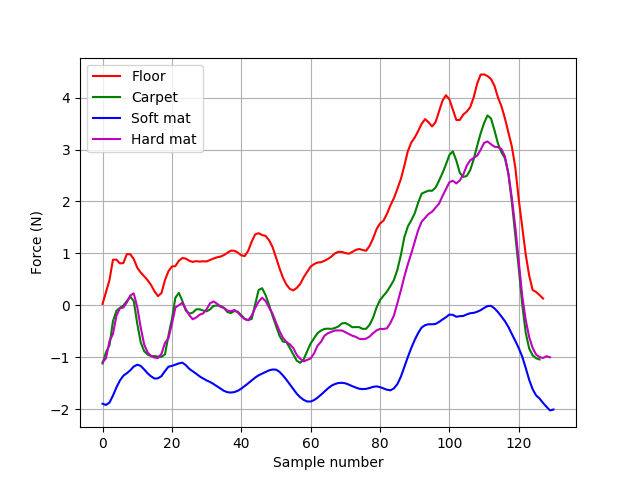
\includegraphics[width=\textwidth,height=\textheight,keepaspectratio]{Figures/meanx}
		\caption{}
		\label{fig:meanx} 
	\end{subfigure}
	
	\begin{subfigure}[b]{0.95\textwidth}
		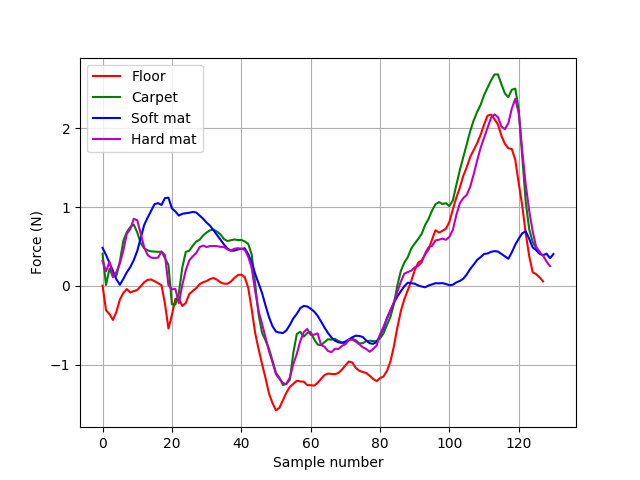
\includegraphics[width=\textwidth,height=\textheight,keepaspectratio]{Figures/meany}
		\caption{}
		\label{fig:meany}
	\end{subfigure}
\end{figure}
	\begin{figure}[h] \ContinuedFloat
	\begin{subfigure}[b]{0.95\textwidth}
		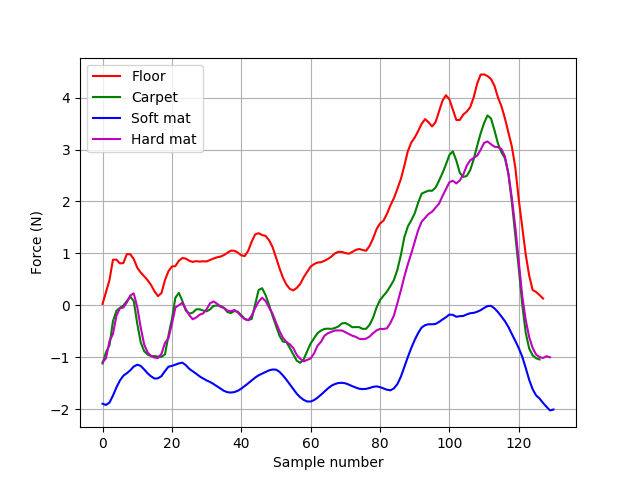
\includegraphics[width=\textwidth,height=\textheight,keepaspectratio]{Figures/meanz}
		\caption{}
		\label{fig:meanz}
	\end{subfigure}
	
	\caption[Two numerical solutions]{(a) Numerical solutions for the small-time system 
		with a constant-curvature body shape showing the scaled leading-order veritcal 
		reaction force $N_0$ versus the scaled body mass $M$ for various values of $g$. 
		Again, $I=M$ for definiteness and $A=0.7$. (b) As for (a) but over a wider range of 
		values of $M,I$.}
	\label{fig:meanxyz}
\end{figure}


\begin{figure}[h]
	\centering
	\begin{subfigure}[b]{0.95\textwidth}
		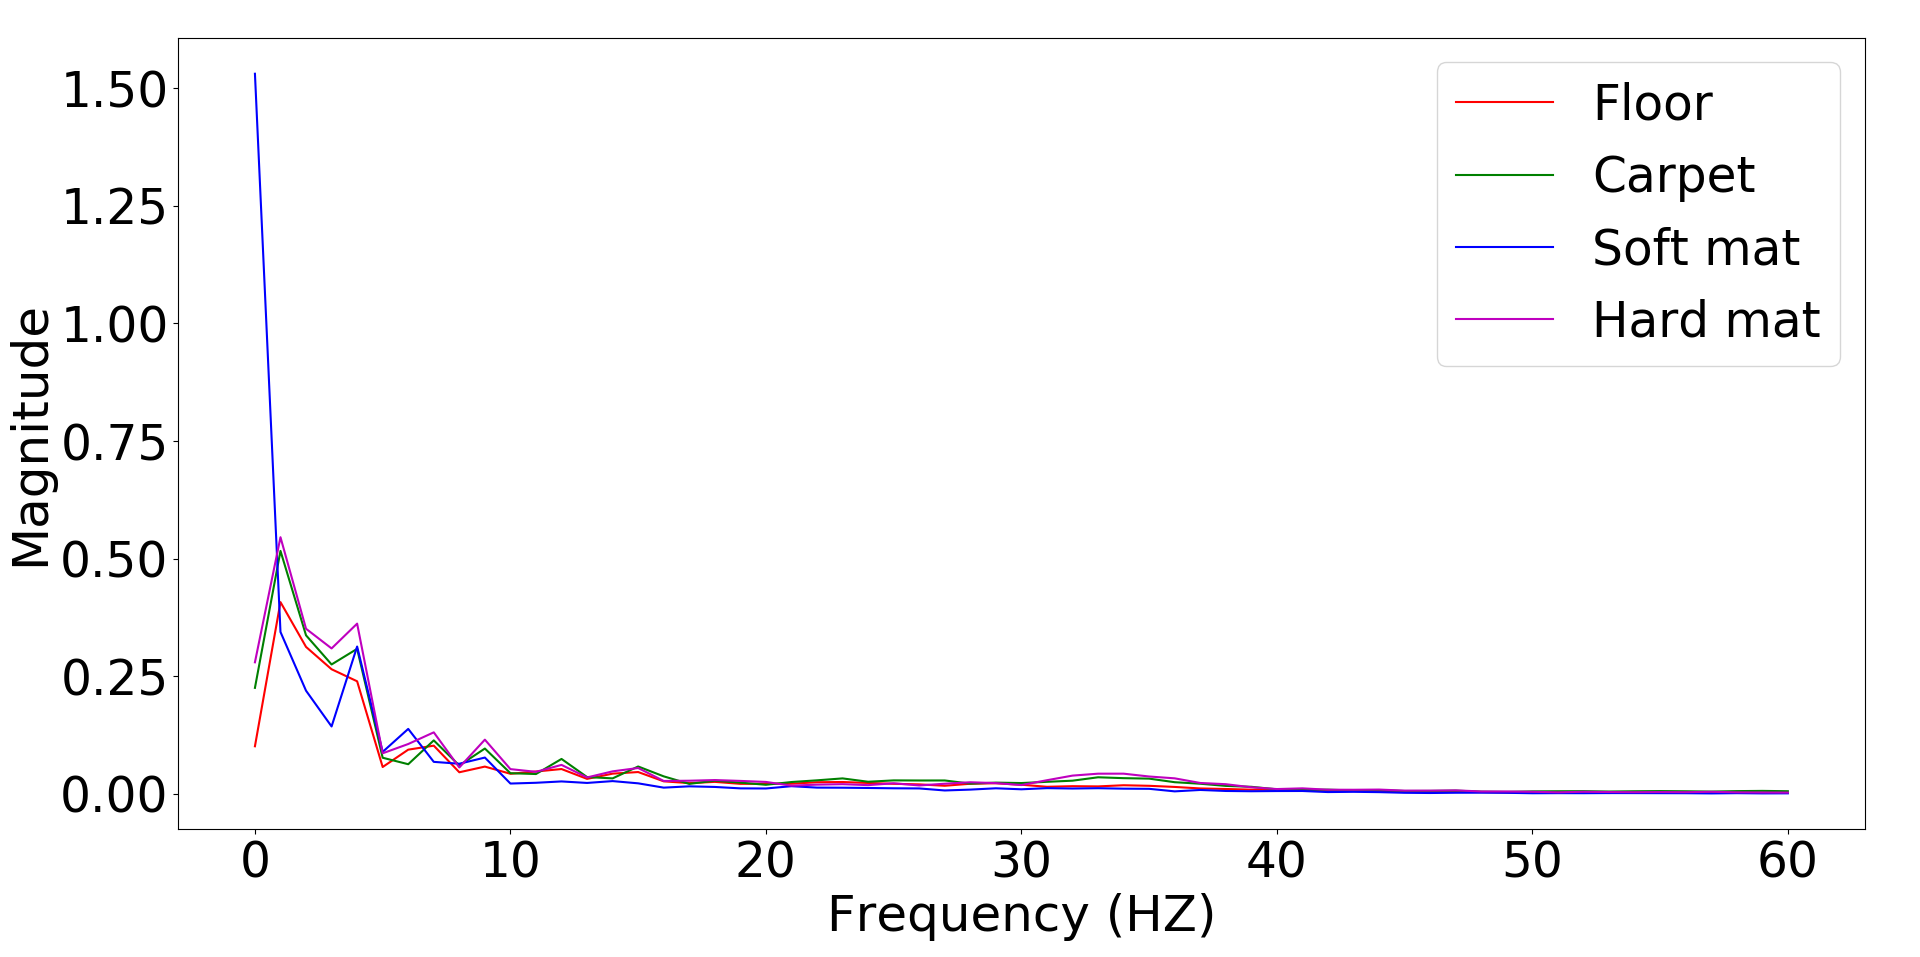
\includegraphics[width=1\linewidth]{Figures/fftx}
		\caption{}
		\label{fig:fftx} 
	\end{subfigure}
\end{figure}
\begin{figure}[h] \ContinuedFloat	
	\begin{subfigure}[b]{0.95\textwidth}
		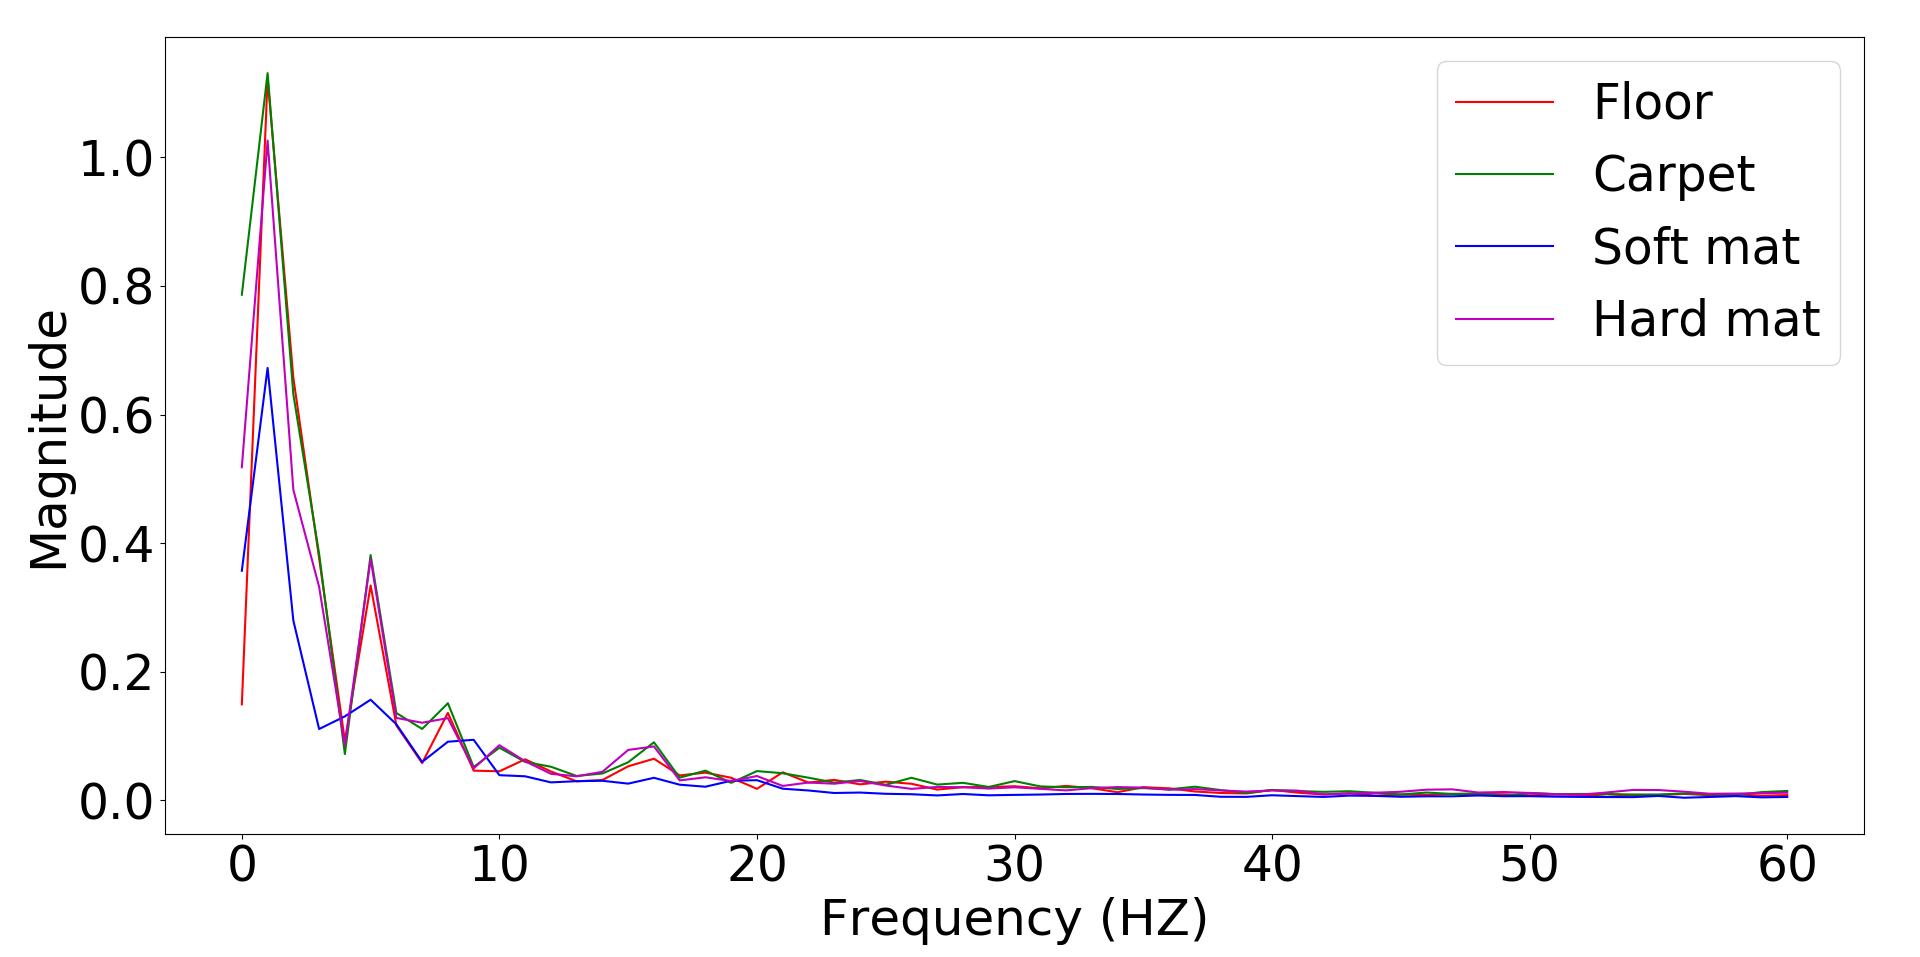
\includegraphics[width=1\linewidth]{Figures/ffty}
		\caption{}
		\label{fig:ffty}
	\end{subfigure}


	\begin{subfigure}[h]{0.95\textwidth}
		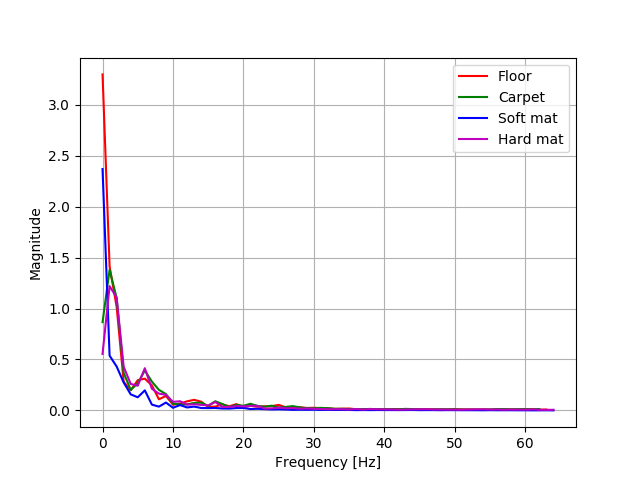
\includegraphics[width=1\linewidth]{Figures/fftz}
		\caption{}
		\label{fig:fftz}
	\end{subfigure}
	
	\caption[Two numerical solutions]{(a) Numerical solutions for the small-time system 
		with a constant-curvature body shape showing the scaled leading-order veritcal 
		reaction force $N_0$ versus the scaled body mass $M$ for various values of $g$. 
		Again, $I=M$ for definiteness and $A=0.7$. (b) As for (a) but over a wider range of 
		values of $M,I$.}
	\label{fig:fftxyz}
\end{figure}
\FloatBarrier

\begin{comment}
\begin{figure}[h]
	\begin{subfigure}{0.5\linewidth}
		\centering
		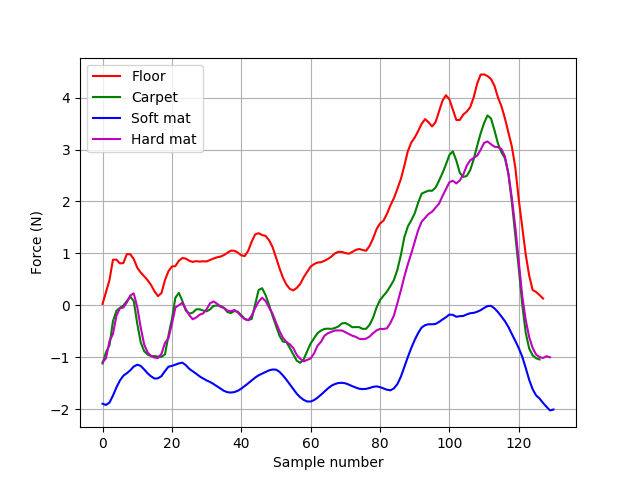
\includegraphics[scale=0.42]{Figures/meanx}
		\caption{}
		\label{fig:sub1}
	\end{subfigure}%
	\begin{subfigure}{.5\linewidth}
		\centering
		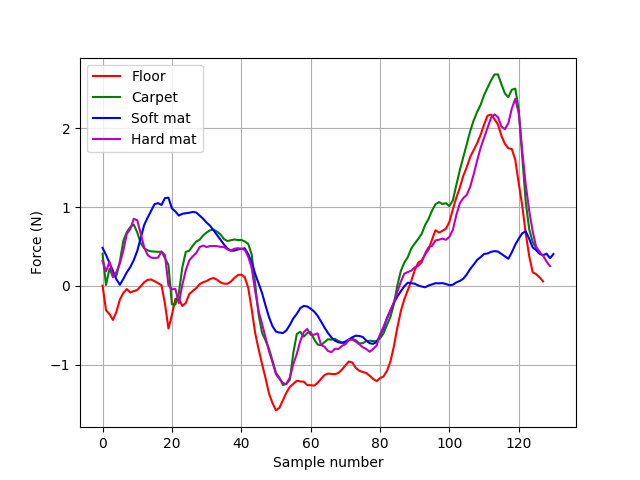
\includegraphics[scale=0.42]{Figures/meany}
		\caption{}
		\label{fig:sub2}
	\end{subfigure}\\[1ex]
	\begin{subfigure}{\linewidth}
		\centering
		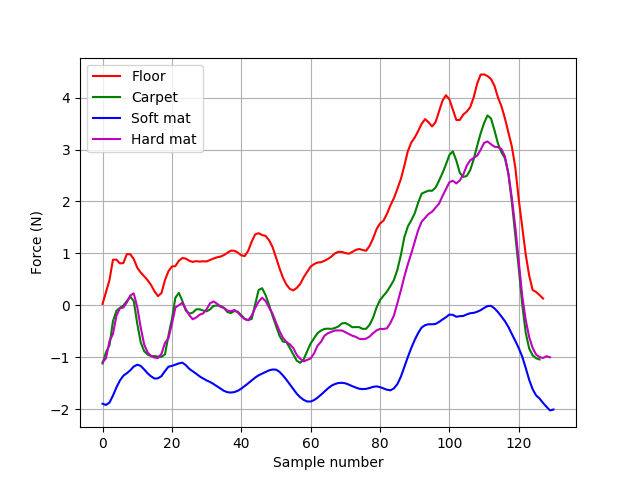
\includegraphics[scale=0.42]{Figures/meanz}
		\caption{}
		\label{fig:sub3}
	\end{subfigure}
	\caption{Figur showing the mean}
	\label{fig:meanx}
\end{figure}
\end{comment}



\begin{comment}
	content...
\begin{figure}[h]
	\begin{subfigure}{0.5\linewidth}
		\centering
		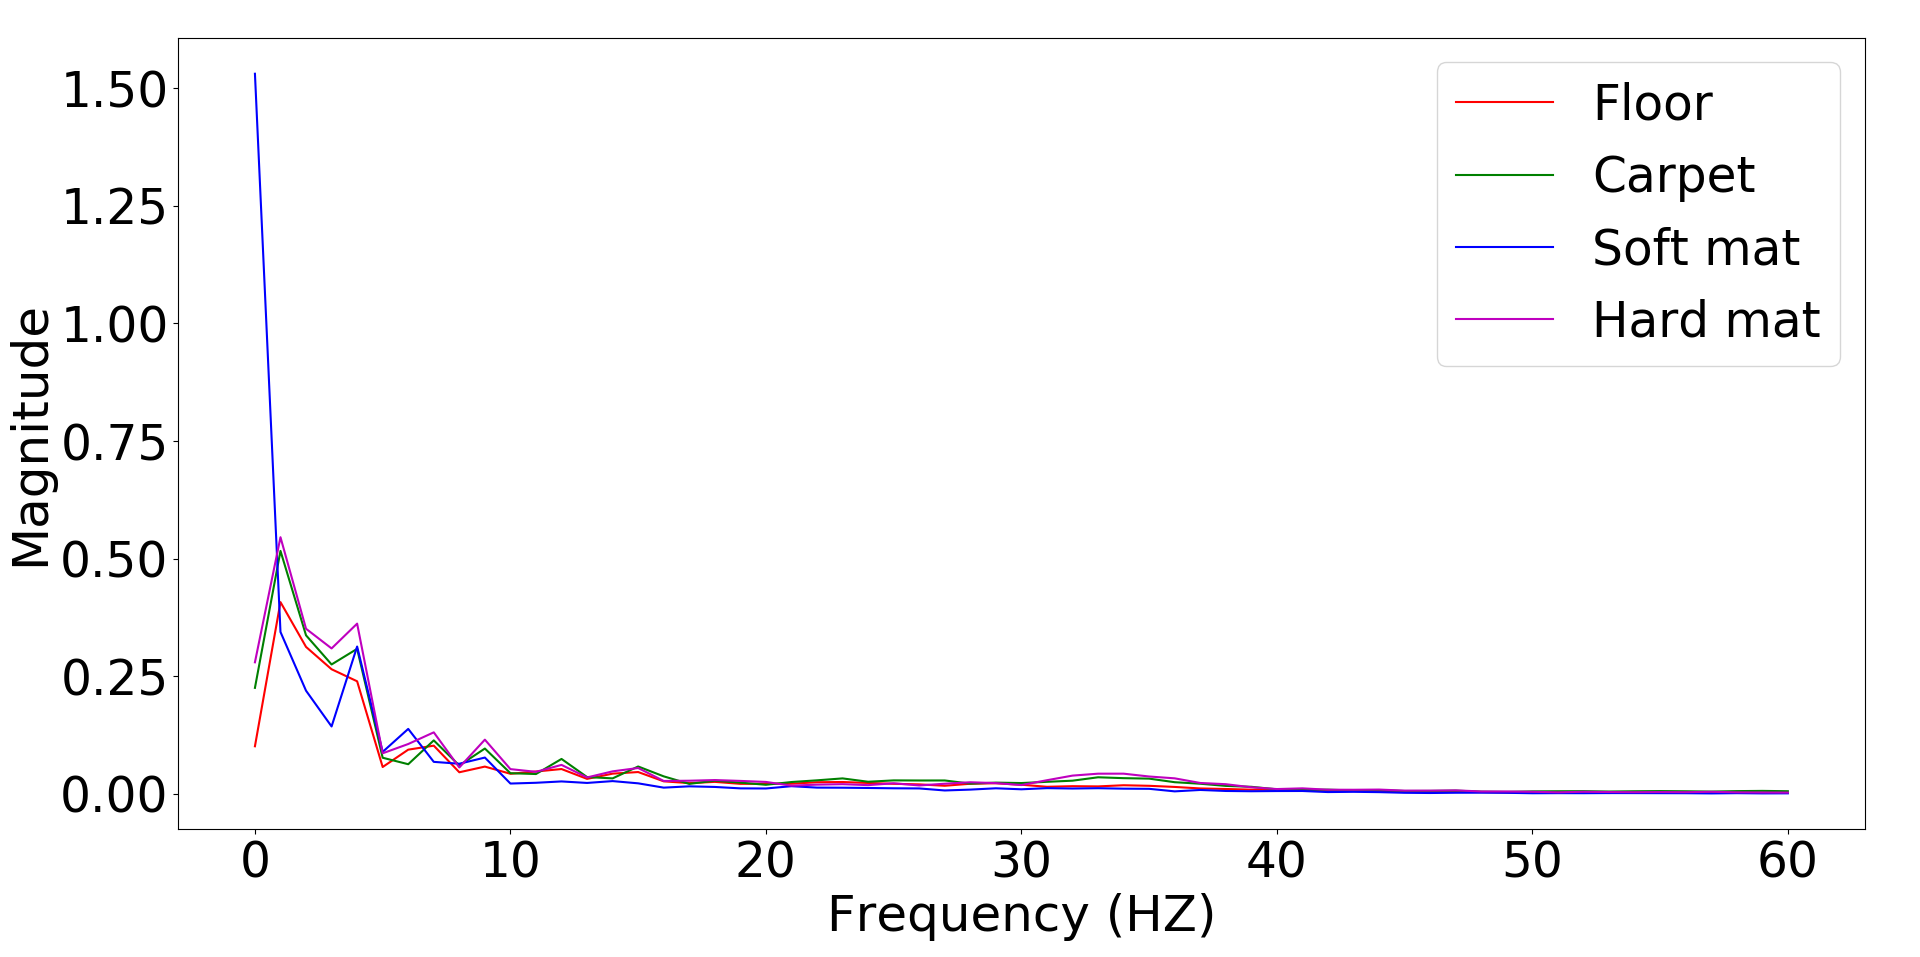
\includegraphics[scale=0.4]{Figures/fftx}
		\caption{}
		\label{fig:sub1}
	\end{subfigure}%
	\begin{subfigure}{.5\linewidth}
		\centering
		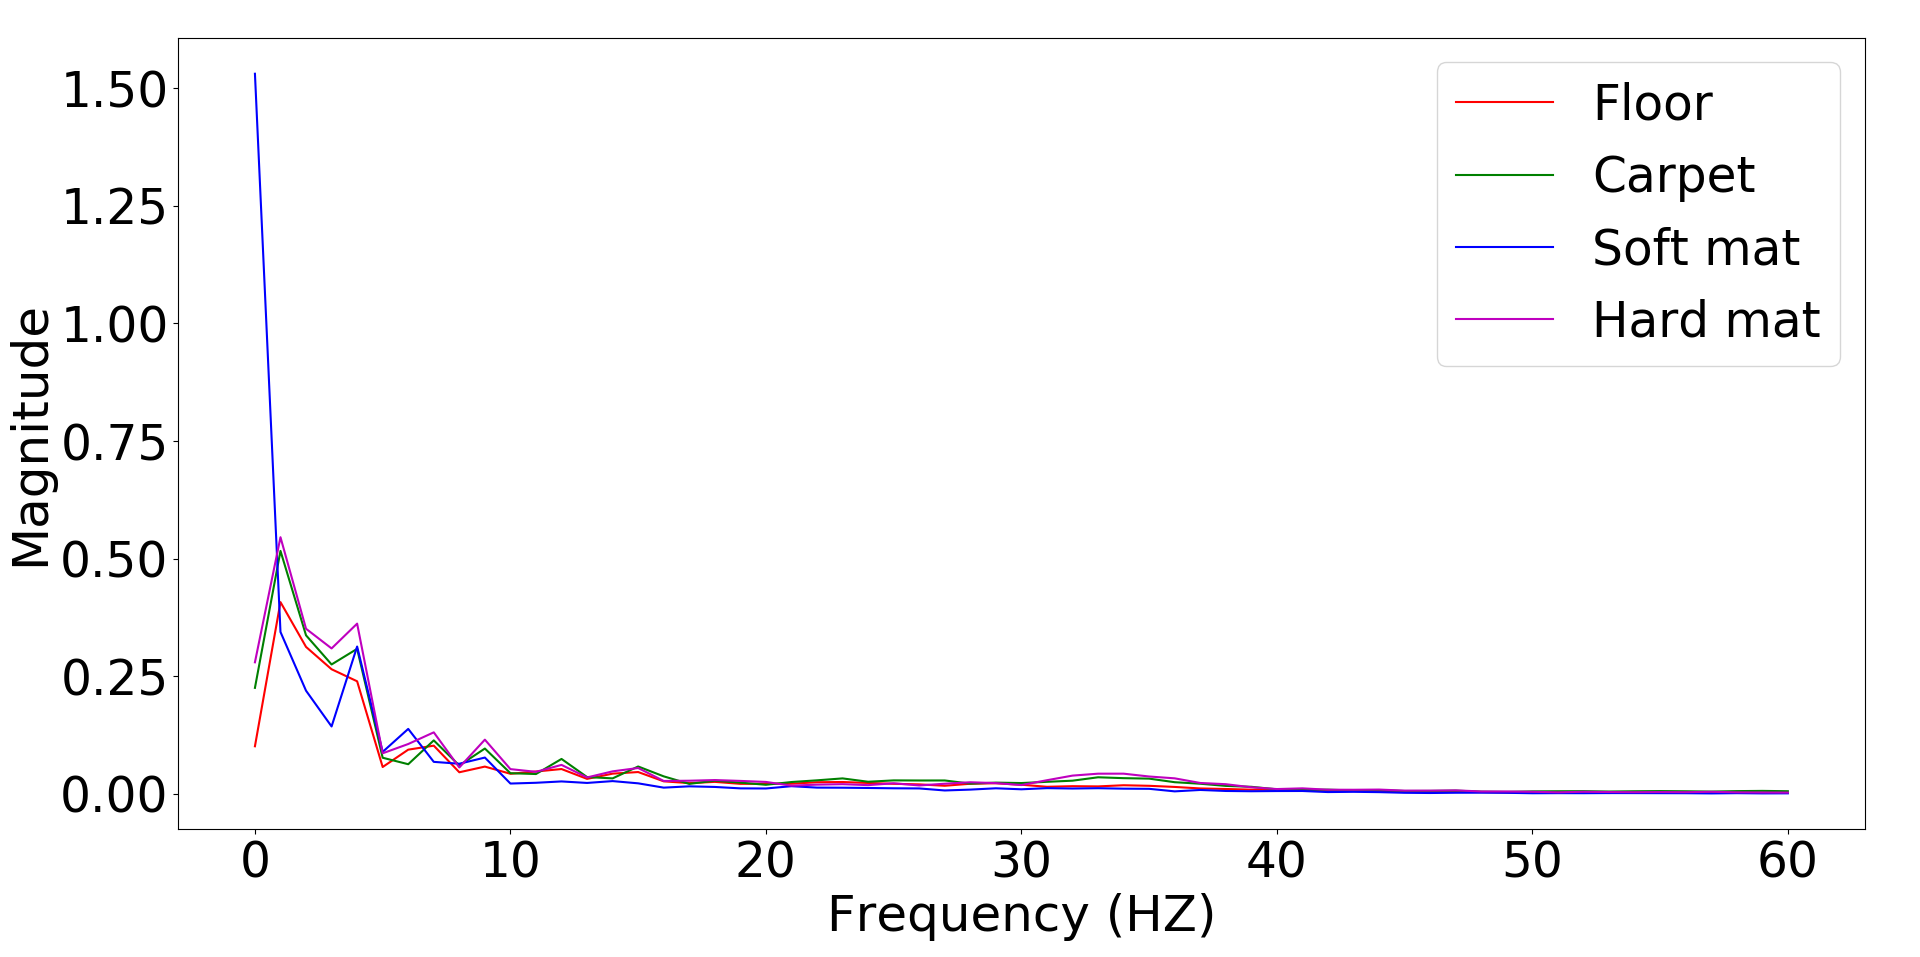
\includegraphics[scale=0.4]{Figures/fftx}
		\caption{}
		\label{fig:sub2}
	\end{subfigure}\\[1ex]
	\begin{subfigure}{\linewidth}
		\centering
		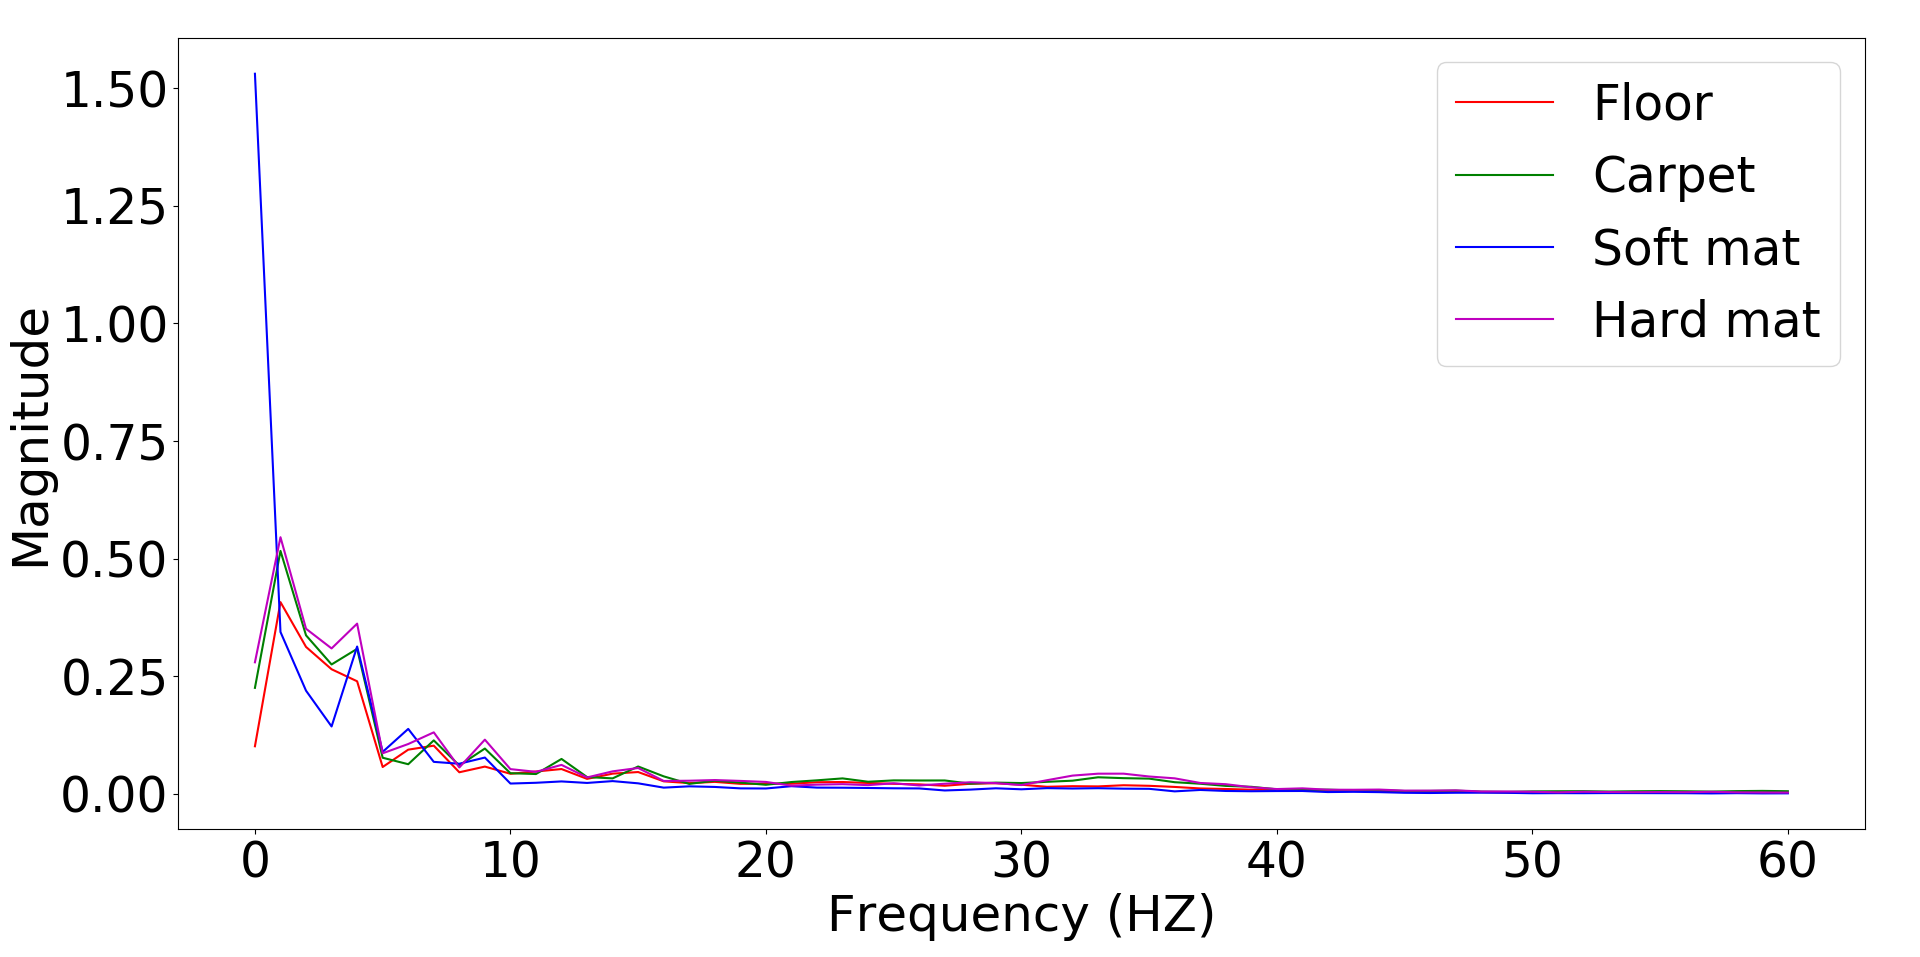
\includegraphics[scale=0.4]{Figures/fftx}
		\caption{}
		\label{fig:sub3}
	\end{subfigure}
	\caption{FFT of }
	\label{fig:fft}
\end{figure}
\end{comment}




\subsection{Feature sets}\label{sec:featuresets}
\paragraph{Feature set one - raw data} This feature set use all of the data from each step in x,y and z-direction. The raw data is decimated in order to achieve a constant length, in this case 125, and compressed into one feature vector. Achieving the fixed length is described in section \ref{subseq:FixLength}. The feature vector can be seen in \ref{eq:f1}.

\begin{equation} \label{eq:f1}
f_{set1}= \left\{ x_1,\dotsc,x_{125},y_1, \dotsc,y_{125},z_1,\dotsc,z_{125} \right\}
\end{equation}
The feature contain 125 feature from each 3 sensors, which mean 375 features.


\paragraph{Feature set two - statistical features} This feature set extracting statistical feature from the dataset. Earlie work is it well used. This is using some of the features from this article \cite{Hoffmann20141790}. The features from this set will be for each direction x,y and z:

\begin{enumerate}
\item The maximum value of the dataset in time domain
\item The minimum value of the dataset in time domain
\item Skew in time domain
\item Kuortosis in time domain 
\item Standard deviation in time domain
\end{enumerate}

The feature set will be look like:

\begin{align}
 f_{set2} &= \left\{ x_{max},x_{min},x_{skew},x_{kuortosis},x_{std},x_{var},x_{trapz}, \right.\nonumber\\
 &\qquad \left. {} y_{max},y_{min},y_{skew},y_{kuortosis},y_{std},y_{var},y_{trapz}, \right.\nonumber\\
 &\qquad \left. {} z_{max},z_{min},z_{skew},z_{kuortosis},z_{std},z_{var},z_{trapz} \right\}
\end{align}

The feature contain 7 features from each direction, which mean total 21 features. 

\paragraph{Feature set three - complete frequency spectrum} Previous work has shown that using frequency has shown good result. In this feature set, the raw data from time domain is transformed into the frequency domain by fft. After tranformation a decimation need to be used, to have a fixed length. 

\begin{equation} \label{eq:f2}
f_{set3}= \left\{ fx_1,\dotsc,fx_{61},fy_1, \dotsc,fy_{61},fz_1,\dotsc,fz_{61} \right\}
\end{equation}


\paragraph{Feature set four - staticial features} This feature set compute the frequency domain of each direction of the raw data. The features mostly same as feature set two and additionally the energy of the spectrum.

\begin{enumerate}
\item The maximum value of the dataset in fequency domain
\item The minimum value of the dataset in fequency domain
\item Skew in fequency domain
\item Kuortosis in fequency domain 
\item Standard deviation in fequency domain
\item Energy 
\end{enumerate}

The feature which will be feed into classifier:
\begin{align}
 f_{set3} &= \left\{ fx_{max},fx_{min},fx_{skew},fx_{kuortosis},fx_{std},fx_{var},fx_{E}, \right.\nonumber\\
 &\qquad \left. {} fy_{max},fy_{min},fy_{skew},fy_{kuortosis},fy_{std},fy_{var},fy_{E}, \right.\nonumber\\
 &\qquad \left. {} fz_{max},fz_{min},fz_{skew},fz_{kuortosis},fz_{std},fz_{var},fz_{E} \right\}
\end{align}

\paragraph{Feature set five - set two and four} Good feature might come from different feature sets. The features from set two and four will be collected as a one set. 
\begin{align}
f_{set5} &= \left\{ x_{max},x_{min},x_{skew},x_{kuortosis},x_{std},x_{var},x_{trapz}, \right.\nonumber\\
&\qquad \left. {}  y_{max},y_{min},y_{skew},y_{kuortosis},y_{std},y_{var},y_{trapz}, \right.\nonumber\\
&\qquad \left. {}  z_{max},z_{min},z_{skew},z_{kuortosis},z_{std},z_{var},z_{trapz}, \right.\nonumber\\
&\qquad \left. {} fx_{max},fx_{min},fx_{skew},fx_{kuortosis},fx_{std},fx_{var},fx_{E}, \right.\nonumber\\
&\qquad \left. {} fy_{max},fy_{min},fy_{skew},fy_{kuortosis},fy_{std},fy_{var},fy_{E}, \right.\nonumber\\
&\qquad \left. {} fz_{max},fz_{min},fz_{skew},fz_{kuortosis},fz_{std},fz_{var},fz_{E} \right\}
\end{align}

\subsection{Achieving a fixed length of the sequences} \label{subseq:FixLength}
In order to use raw data as input, an fixed length is required. The steps have been decimated in order for to achieve a constant length of 125. It is shown that each step is vary between 125-135. A simplified method for achieving fixed length is shown. Note the technique is simplified to one-dimensional array, while in thesis has 3 dimensional array, but the intention is same. Using this technique it is considerate that data in end and start are less important than in middle.
  
\begin{lstlisting}[language=Python]

def fix_length(data_sequence):
    fixed_length = 125
    total_length = len(data_sequence)  
    total_cut = total_length-fixed_length

    #In case the sequence is odd
    rest = total_cut%2
    
    #Calculate the start and end position
    start_pos = total_cut/2 
    end_pos = total_length - (total_cut/2)+rest 

    #Retrieve fixed sequense data 
    fixed_data_sequence = data_sequence[start_pos:end_pos] 
    return fixed_data_sequence
\end{lstlisting}

\newpage
\section{Learning approach}
The learning approach is divided into to processes. First to divide the file and learning process.

\subsection{Collecting samples}
The samples used as training and test is a step before the learning procedure. This is to gather data sample for each terrain into a file, which will be used in the learning process. The procedure is shown in figure \ref{fig:createsamples}

\begin{figure}[h]
	\centering
	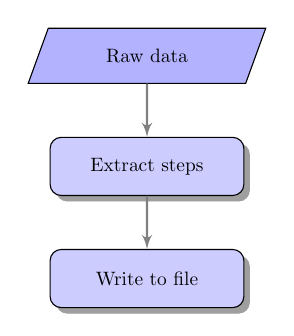
\begin{tikzpicture}[scale=0.7,transform shape]
	
	% Draw diagram elements
	\path \io{1}{Raw data};
	
	\path (p1.south)+(0,-1.5) \etape{2}{Extract steps};
	\path (p2.south)+(0.0,-1.5) \etape{3}{Write to file};
	

	%  \node [below=of p5] (p6-7) {};
	
	% Draw arrows between elements
	\path [line] (p1.south) -- node [above] {} (p2);
	\path [line] (p2.south) -- node [above] {} (p3);
	\end{tikzpicture}

\caption{The figure showing steps } \label{fig:createsamples}
\end{figure}

\subsubsection{Procedure of creating samples} \label{sub:createsamples}
\begin{enumerate}
	\item \textbf{\underline{Raw data}}
	\\
	The dataset is retrieved from the optical force sensor.
	
	\item \textbf{\underline{Extract steps}}
	\\
	Raw data will be partitioned into samples as described in section \ref{subseq:segmentation}.
	
	\item \textbf{\underline{Write to file}}
	\\
	This step will write each of data sequence into file with label of the terrain name.
	

\end{enumerate}

\subsection{Learning procedure}
When the data samples of each terrain is collected into a file, the learning process is shown in figure \ref{fig:learningProcess}.
\begin{figure}[h]
\centering
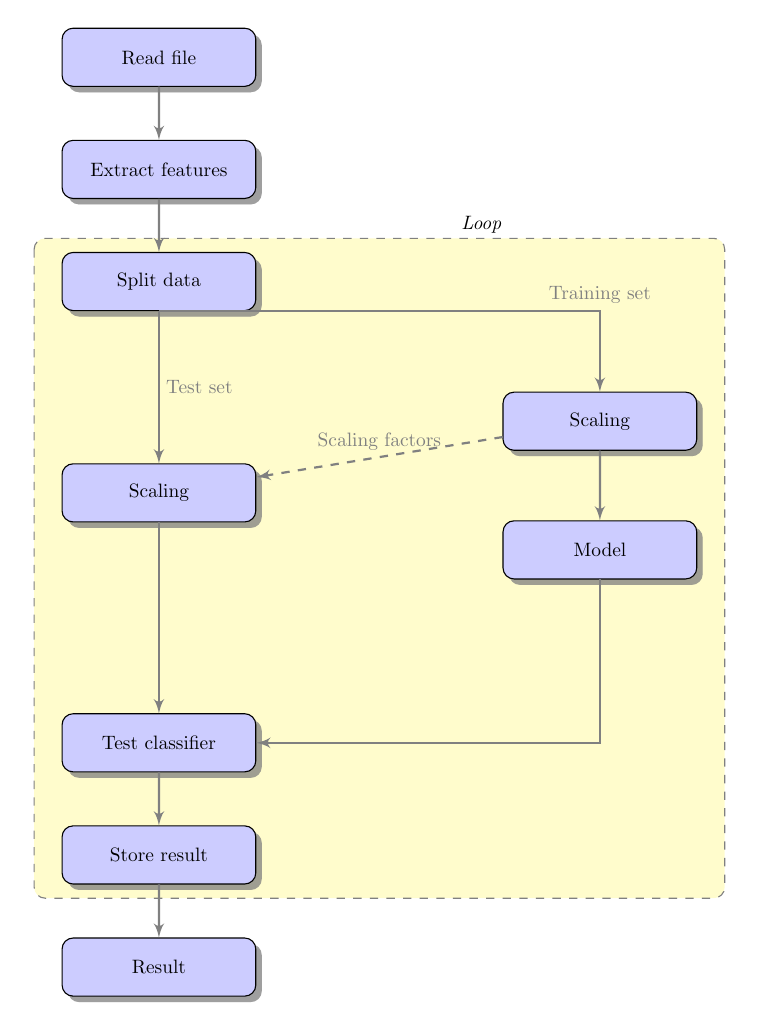
\begin{tikzpicture}[scale=0.7,transform shape]

  % Draw diagram elements
  
  \path \etape{2}{Read file};
  \path (p2.south)+(0.0,-1.5) \etape{3}{Extract features};

  \path (p3.south)+(0.0,-1.5) \etape{4}{Split data};
  \path (p4.south)+(8,-2.0) \etape{5}{Scaling};
  \path (p5.south)+(0,-1.8) \etape{6}{Model};
  \path (p4.south)+(0,-3.3) \etape{9}{Scaling};
  \path (p9.south)+(0,-4.0) \etape{7}{Test classifier};
  
  \path (p7.south)+(0,-1.5) \etape{10}{Store result};
  \path (p10.south)+(0,-1.5) \etape{8}{Result};
    
%  \node [below=of p5] (p6-7) {};

  % Draw arrows between elements
 
  \path [line] (p2.south) -- node [above] {} (p3);
  \path [line] (p3.south) -- node [above] {} (p4);
  \path [line] (p4.south) -| node [above] {Training set} (p5);
    
  \path [line] (p5.south) -- node [above] {} (p6);
  \path [line] (p6.south) |- node [above] {} (p7);
  \path [line] (p4.south) -- node [right] {Test set} (p9);
  \path [line] (p7.south) -- node [above] {} (p10);
  \path [line] (p10.south) -- node [above] {} (p8);
  \path [line] (p9.south) -- node [above] {} (p7);
%  \path [line] (p5.south) -- node [above] {Feature} (p9);
   \path [line,dashed] (p5) -- node [above]{Scaling factors} (p9);
  \background{p3}{p4}{p5}{p10}{Loop} 
  
\end{tikzpicture}



\caption{The figure showing steps } \label{fig:learningProcess}
\end{figure}

\FloatBarrier

\subsubsection{Details of the learning process}
\begin{enumerate}
\item \textbf{\underline{Reading file with samples}}
\\
This step will take a file as input, created from section \ref{sub:createsamples}.

\item \textbf{\underline{Extract features}}
\\
This step will create one of the five feature sets as mentioned in section \ref{sec:featuresets}.

\item \textbf{\underline{Loop}}

\begin{enumerate} 
\item \textbf{\underline{Split data}} \label{en:loop}
\\
\\
The extracted feature vectors is partitioned into a training and testing set. The cross validation is LOOCV, thus the training set consists of 199 samples and one test sample.


\item \textbf{\underline{Scaling}}
\\
This step takes the training set as input and standardization as mention in section \ref{subsec:scaling}. It will first scale the training data, and then scaling factors are applied to the test data.

Scale first the training set and then transform the testing set.
\item \textbf{\underline{Train the classifier}}
\\
The classifier will take the training set as input and train.

\item \textbf{\underline{Test classifier}} This step use the model to predict the test set. It will store the score.


\item \textbf{\underline{Store result}} This step will store the result of the test sample.If there are still more data to be predicted start from \ref{en:loop}.

\end{enumerate}


\item \textbf{\underline{Result}}
\\
\\
Compute the average results as mentioned in section \ref{subsec:evalclf} 
\end{enumerate}



\chapter{Experiments and results}                     %% ... or ??
The chapter present the results of all model in previous chapter. The two-class classification will be investigated first. Further will be to using methods to improve each of classifier. The best classifier will be used to test. 

\section{Results of classifier}\label{result_exp1}
Table \ref{exp1} shows the result when using the learning approach. The accuracy is the average accuracy. The experiments were done twice, both with and without the feature scaling. 


\begin{table}[]
\centering
\resizebox{\textwidth}{!}{%
\begin{tabular}{@{}l|l|l|l@{}}
\toprule
\multirow{2}{*}{\textbf{Feature set}} & \multirow{2}{*}{\textbf{Classifier}} & \multicolumn{2}{c|}{\textbf{Accuracy}} \\ \cmidrule(l){3-4} 
 &  & \textbf{Not scaled} & \textbf{Scaled} \\ \midrule
\multirow{6}{*}{\begin{tabular}[c]{@{}l@{}}Set one -\\ raw data\end{tabular}} & \multirow{2}{*}{Bayes Navies} & \multirow{2}{*}{0.83} & \multirow{2}{*}{0.83} \\
 &  &  &  \\ \cmidrule(l){2-4} 
 & Decision tree & 0.94 & 0.96 \\ \cmidrule(l){2-4} 
 & KNN & 0.89 & 0.91 \\ \cmidrule(l){2-4} 
 & Neural network & 0.95 & 0.96 \\ \cmidrule(l){2-4} 
 & SVM & 0.89 & 0.93 \\ \midrule
\multirow{5}{*}{\begin{tabular}[c]{@{}l@{}}Set two - \\ statistical features in \\ time domain\end{tabular}} & Bayes Navies & 0.82 & 0.82 \\ \cmidrule(l){2-4} 
 & Decision tree & 0.83 & 0.84 \\ \cmidrule(l){2-4} 
 & KNN & 0.84 & 0.84 \\ \cmidrule(l){2-4} 
 & Neural network & 0.83 & 0.88 \\ \cmidrule(l){2-4} 
 & SVM & 0.76 & 0.85 \\ \midrule
\multirow{5}{*}{\begin{tabular}[c]{@{}l@{}}Set three - \\ complete frequency \\ domain\end{tabular}} & Bayes Navies & 0.91 & 0.91 \\ \cmidrule(l){2-4} 
 & Decision tree & 0.83 & 0.82 \\ \cmidrule(l){2-4} 
 & KNN & 0.91 & 0.88 \\ \cmidrule(l){2-4} 
 & Neural network & 0.93 & 0.93 \\ \cmidrule(l){2-4} 
 & SVM & 0.52 & 0.93 \\ \midrule
\multirow{5}{*}{\begin{tabular}[c]{@{}l@{}}Set four - \\ staticial features in \\ frequency domain\end{tabular}} & Bayes Navies & 0.81 & 0.81 \\ \cmidrule(l){2-4} 
 & Decision tree & 0.80 & 0.82 \\ \cmidrule(l){2-4} 
 & KNN & 0.88 & 0.84 \\ \cmidrule(l){2-4} 
 & Neural network & 0.85 & 0.88 \\ \cmidrule(l){2-4} 
 & SVM & 0.83 & 0.86 \\ \midrule
\multirow{5}{*}{\begin{tabular}[c]{@{}l@{}}Set five - \\ set 2,4\end{tabular}} & Bayes Navies & 0.82 & 0.82 \\ \cmidrule(l){2-4} 
 & Decision tree & 0.79 & 0.80 \\ \cmidrule(l){2-4} 
 & KNN & 0.88 & 0.84 \\ \cmidrule(l){2-4} 
 & Neural network & 0.87 & 0.89 \\ \cmidrule(l){2-4} 
 & SVM & 0.83 & 0.86 \\ \bottomrule
\end{tabular}%
}
\caption{My caption}
\label{exp1}
\end{table}

\FloatBarrier


\subsection{Analysis}
The result shown that all classifier has a accuracy at least 70\%. The Decision tree and Neural Network has the highest accuracy with 96\% from scaled feature set one. 
\\
\\
Regarding the feature scaling, SVM classifer is the one with huge affect of the scaled. The KNN which is also distances is also affected by scaling, but most of them gave lesser accuracy. While Neural Network, Decision tree and Bayes Navies do not rely on distance between features, only Bayes Navies was not affected. The Neural Network and Decision Tree had minor change in their accuracy. Since the feature scaling had great affect on the SVM and minor on the other classifier, scaled features will be used in further experiments.
\\
\\
Note that the mostly higest result is from features with whole sequencse. The benefit of using raw data is ensuring that all the information is in the data. The more data might be easier to recognize a pattern or find characteristic for each terrain. Conversely, by extraction features might loose important features, hence to not high accuracy.
\\
\\
Even there are two classifier which outpeform the other, there are still a improving potensial to all of them. The improvement will be investigated in next section.



\section{Further improving all classifier}
The classifier approach state earlier has leaved the feature selection out. The reason was to see how well each classifier predicted terrain based on all features. It has shown in section \ref{result_exp1} that it gave high accuracy for most of them. As stated in section \ref{selection}, selecting good features has benefit of increasing classifier perfomance. In this approach feature selection is implemented into the earlier approach. Two different feature selection methods is tested, filter and wrapper.

\begin{figure}[h!]
\centering
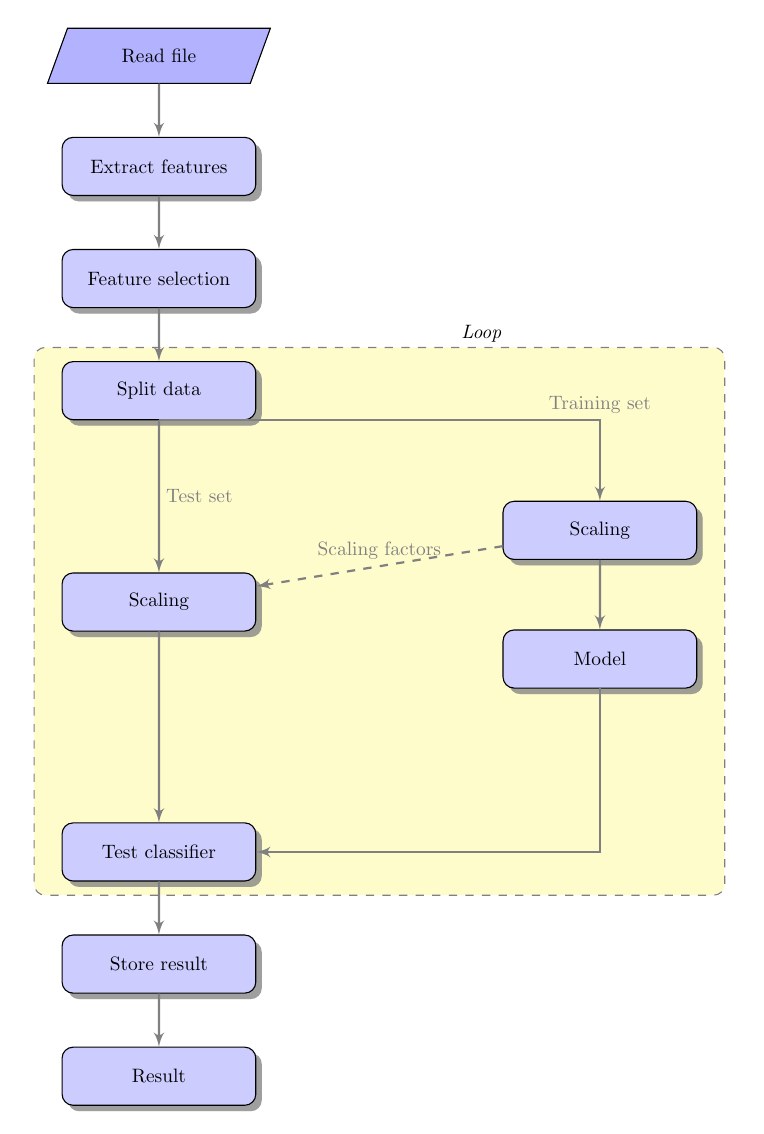
\begin{tikzpicture}[scale=0.7,transform shape]

  % Draw diagram elements
%  \path \io{1}{Raw data};
  \path \io{2}{Read file};
%  \path (p1.south)+(0,-1.5) \etape{2}{Extract steps};
  \path (p2.south)+(0.0,-1.5) \etape{3}{Extract features};
  \path (p3.south)+(0.0,-1.5) \etape{11}{Feature selection};
  
  \path (p11.south)+(0.0,-1.5) \etape{4}{Split data};
  \path (p4.south)+(8,-2.0) \etape{5}{Scaling};
  \path (p5.south)+(0,-1.8) \etape{6}{Model};
  \path (p4.south)+(0,-3.3) \etape{9}{Scaling};
  \path (p9.south)+(0,-4.0) \etape{7}{Test classifier};
  
  \path (p7.south)+(0,-1.5) \etape{10}{Store result};
  \path (p10.south)+(0,-1.5) \etape{8}{Result};
    
%  \node [below=of p5] (p6-7) {};

  % Draw arrows between elements
 % \path [line] (p1.south) -- node [above] {} (p2);
  \path [line] (p2.south) -- node [above] {} (p3);
  \path [line] (p3.south) -- node [above] {} (p11);
  \path [line] (p11.south) -- node [above] {} (p4);
  \path [line] (p4.south) -| node [above] {Training set} (p5);
    
  \path [line] (p5.south) -- node [above] {} (p6);
  \path [line] (p6.south) |- node [above] {} (p7);
  \path [line] (p4.south) -- node [right] {Test set} (p9);
  \path [line] (p7.south) -- node [above] {} (p10);
  \path [line] (p10.south) -- node [above] {} (p8);
  \path [line] (p9.south) -- node [above] {} (p7);
%  \path [line] (p5.south) -- node [above] {Feature} (p9);
   \path [line,dashed] (p5) -- node [above]{Scaling factors} (p9);
  \background{p3}{p4}{p5}{p7}{Loop} 
  
\end{tikzpicture}

\caption{The figure showing steps } \label{fig:M1}
\end{figure}


\section{Experiment 2 - classifier improvement}
Table \ref{exp2} shows the result when using the learning approach. The accuracy is the average accuracy. The experiments were done twice, both with filter and wrapper method.


\begin{table}[]
\centering
\resizebox{\textwidth}{!}{%
\begin{tabular}{@{}l|l|l|l|l@{}}
\toprule
\multirow{2}{*}{\textbf{Feature set}} & \multirow{2}{*}{\textbf{Classifier}} & \multicolumn{3}{c|}{\textbf{Accuracy}} \\ \cmidrule(l){3-5} 
 &  & \textbf{Old result} & \textbf{Filter} & \textbf{Wrapper} \\ \midrule
\multirow{5}{*}{\begin{tabular}[c]{@{}l@{}}Set one -\\ raw data\end{tabular}} & Bayes Navies & 0.83 & 0.78 & 0.81 \\ \cmidrule(l){2-5} 
 & Decision tree & 0.96 & 0.96 & 0.93 \\ \cmidrule(l){2-5} 
 & KNN & 0.91 & 0.95 & 0.93 \\ \cmidrule(l){2-5} 
 & Neural network & 0.96 & 0.94 & 0.95 \\ \cmidrule(l){2-5} 
 & SVM & 0.93 & 0.91 & 0.94 \\ \midrule
\multirow{5}{*}{\begin{tabular}[c]{@{}l@{}}Set two - \\ statistical features in \\ time domain\end{tabular}} & Bayes Navies & 0.82 & 0.74 & 0.84 \\ \cmidrule(l){2-5} 
 & Decision tree & 0.84 & 0.79 & 0.81 \\ \cmidrule(l){2-5} 
 & KNN & 0.84 & 0.82 & 0.82 \\ \cmidrule(l){2-5} 
 & Neural network & 0.88 & 0.81 & 0.84 \\ \cmidrule(l){2-5} 
 & SVM & 0.85 & 0.80 & 0.83 \\ \midrule
\multirow{5}{*}{\begin{tabular}[c]{@{}l@{}}Set three - \\ complete frequency \\ domain\end{tabular}} & Bayes Navies & 0.91 & 0.76 & 0.94 \\ \cmidrule(l){2-5} 
 & Decision tree & 0.82 & 0.76 & 0.81 \\ \cmidrule(l){2-5} 
 & KNN & 0.88 & 0.83 & 0.91 \\ \cmidrule(l){2-5} 
 & Neural network & 0.93 & 0.78 & 0.95 \\ \cmidrule(l){2-5} 
 & SVM & 0.93 & 0.79 & 0.97 \\ \midrule
\multirow{5}{*}{\begin{tabular}[c]{@{}l@{}}Set four - \\ staticial features in \\ frequency domain\end{tabular}} & Bayes Navies & 0.81 & 0.75 & 0.79 \\ \cmidrule(l){2-5} 
 & Decision tree & 0.82 & 0.82 & 0.81 \\ \cmidrule(l){2-5} 
 & KNN & 0.84 & 0.85 & 0.86 \\ \cmidrule(l){2-5} 
 & Neural network & 0.88 & 0.84 & 0.90 \\ \cmidrule(l){2-5} 
 & SVM & 0.86 & 0.82 & 0.86 \\ \midrule
\multirow{5}{*}{\begin{tabular}[c]{@{}l@{}}Set five - \\ set 2,4\end{tabular}} & Bayes Navies & 0.82 & 0.74 & 0.84 \\ \cmidrule(l){2-5} 
 & Decision tree & 0.80 & 0.82 & 0.84 \\ \cmidrule(l){2-5} 
 & KNN & 0.84 & 0.86 & 0.83 \\ \cmidrule(l){2-5} 
 & Neural network & 0.89 & 0.81 & 0.89 \\ \cmidrule(l){2-5} 
 & SVM & 0.86 & 0.83 & 0.86 \\ \bottomrule
\end{tabular}%
}
\caption{My caption}
\label{exp2}
\end{table}
\FloatBarrier

\section{Analysis}
From table \label{exp2} one can see that the filter selection has made the classifier more inaccurate. It seems that important features were removed. As in section. that one feature may not be important by itself, but might be important to others. The wrapper selection, on the other hand, provide a significant better result compared to the filter. It also has improved the SVM to 97\% accuracy.
\\
\\
Note that the k-fold validation test using always use the same single set both for training and testing, which make it reffering to themselve than to generalize model of particular terrain class. In this case results from \ref{exp2} only gives an estimation on how well a classifier is, but does not tell how well it predict on unseen data. One way to avoid this issue is make the training set and testing set independed to each other, then the predicition will predict on new data in the k-fold \cite{hexapod}. The following experiment only four of the highest classifier shown in \ref{exp2} would be investigated further. As there are 3 second best classifier, all of them will be in further experiments. This is divided into further experiments.

\section{Cross validation with unseen data}
In this experiment 50 new samlpes for each terrain is collected. This is divided into further experiments to comparing the two best classifier.

\begin{enumerate}
\item SVM with wrapper and use feature set two
\item Neural Network and use feature set one.
\item Decision tree with feature set one
\item Decision tree with filter and use feature set one
\end{enumerate}
Note the training set and test set will be randomly shuffled, which might cause an inaccurate measurement of classifier. To achieve more accuracy measure of classifier, each test will be runned five times.


\begin{table}[h]
\centering
\resizebox{\textwidth}{!}{%
\begin{tabular}{@{}llllllll@{}}
\toprule
\multirow{2}{*}{Run} & \multirow{2}{*}{Accuracy} & \multirow{2}{*}{Precision} & \multirow{2}{*}{Recall} & \multicolumn{4}{c}{Confusion matrix} \\ \cmidrule(l){5-8} 
 &  &  &  & \multicolumn{1}{l|}{Floor} & \multicolumn{1}{l|}{Carpet} & \multicolumn{1}{l|}{Soft mat} & Hard mat \\ \midrule
\multicolumn{1}{l|}{\multirow{4}{*}{1}} & \multicolumn{1}{l|}{\multirow{4}{*}{0.97}} & \multicolumn{1}{l|}{\multirow{4}{*}{p1}} & \multicolumn{1}{l|}{\multirow{4}{*}{r1}} & \multicolumn{1}{l|}{50} & \multicolumn{1}{l|}{0} & \multicolumn{1}{l|}{0} & 0 \\ \cmidrule(l){5-8} 
\multicolumn{1}{l|}{} & \multicolumn{1}{l|}{} & \multicolumn{1}{l|}{} & \multicolumn{1}{l|}{} & \multicolumn{1}{l|}{2} & \multicolumn{1}{l|}{48} & \multicolumn{1}{l|}{0} & 0 \\ \cmidrule(l){5-8} 
\multicolumn{1}{l|}{} & \multicolumn{1}{l|}{} & \multicolumn{1}{l|}{} & \multicolumn{1}{l|}{} & \multicolumn{1}{l|}{0} & \multicolumn{1}{l|}{0} & \multicolumn{1}{l|}{50} & 0 \\ \cmidrule(l){5-8} 
\multicolumn{1}{l|}{} & \multicolumn{1}{l|}{} & \multicolumn{1}{l|}{} & \multicolumn{1}{l|}{} & \multicolumn{1}{l|}{2} & \multicolumn{1}{l|}{1} & \multicolumn{1}{l|}{0} & 47 \\ \midrule
\multicolumn{1}{l|}{\multirow{4}{*}{2}} & \multicolumn{1}{l|}{\multirow{4}{*}{0.97}} & \multicolumn{1}{l|}{\multirow{4}{*}{p2}} & \multicolumn{1}{l|}{\multirow{4}{*}{r2}} & \multicolumn{1}{l|}{50} & \multicolumn{1}{l|}{0} & \multicolumn{1}{l|}{0} & 0 \\ \cmidrule(l){5-8} 
\multicolumn{1}{l|}{} & \multicolumn{1}{l|}{} & \multicolumn{1}{l|}{} & \multicolumn{1}{l|}{} & \multicolumn{1}{l|}{2} & \multicolumn{1}{l|}{48} & \multicolumn{1}{l|}{0} & 0 \\ \cmidrule(l){5-8} 
\multicolumn{1}{l|}{} & \multicolumn{1}{l|}{} & \multicolumn{1}{l|}{} & \multicolumn{1}{l|}{} & \multicolumn{1}{l|}{0} & \multicolumn{1}{l|}{0} & \multicolumn{1}{l|}{50} & 0 \\ \cmidrule(l){5-8} 
\multicolumn{1}{l|}{} & \multicolumn{1}{l|}{} & \multicolumn{1}{l|}{} & \multicolumn{1}{l|}{} & \multicolumn{1}{l|}{2} & \multicolumn{1}{l|}{1} & \multicolumn{1}{l|}{0} & 47 \\ \midrule
\multicolumn{1}{l|}{\multirow{4}{*}{3}} & \multicolumn{1}{l|}{\multirow{4}{*}{0.97}} & \multicolumn{1}{l|}{\multirow{4}{*}{p3}} & \multicolumn{1}{l|}{\multirow{4}{*}{r3}} & \multicolumn{1}{l|}{50} & \multicolumn{1}{l|}{0} & \multicolumn{1}{l|}{0} & 0 \\ \cmidrule(l){5-8} 
\multicolumn{1}{l|}{} & \multicolumn{1}{l|}{} & \multicolumn{1}{l|}{} & \multicolumn{1}{l|}{} & \multicolumn{1}{l|}{2} & \multicolumn{1}{l|}{48} & \multicolumn{1}{l|}{0} & 0 \\ \cmidrule(l){5-8} 
\multicolumn{1}{l|}{} & \multicolumn{1}{l|}{} & \multicolumn{1}{l|}{} & \multicolumn{1}{l|}{} & \multicolumn{1}{l|}{0} & \multicolumn{1}{l|}{0} & \multicolumn{1}{l|}{50} & 0 \\ \cmidrule(l){5-8} 
\multicolumn{1}{l|}{} & \multicolumn{1}{l|}{} & \multicolumn{1}{l|}{} & \multicolumn{1}{l|}{} & \multicolumn{1}{l|}{2} & \multicolumn{1}{l|}{1} & \multicolumn{1}{l|}{0} & 47 \\ \midrule
\multicolumn{1}{l|}{\multirow{4}{*}{4}} & \multicolumn{1}{l|}{\multirow{4}{*}{0.97}} & \multicolumn{1}{l|}{\multirow{4}{*}{p4}} & \multicolumn{1}{l|}{\multirow{4}{*}{r4}} & \multicolumn{1}{l|}{50} & \multicolumn{1}{l|}{0} & \multicolumn{1}{l|}{0} & 0 \\ \cmidrule(l){5-8} 
\multicolumn{1}{l|}{} & \multicolumn{1}{l|}{} & \multicolumn{1}{l|}{} & \multicolumn{1}{l|}{} & \multicolumn{1}{l|}{2} & \multicolumn{1}{l|}{48} & \multicolumn{1}{l|}{0} & 0 \\ \cmidrule(l){5-8} 
\multicolumn{1}{l|}{} & \multicolumn{1}{l|}{} & \multicolumn{1}{l|}{} & \multicolumn{1}{l|}{} & \multicolumn{1}{l|}{0} & \multicolumn{1}{l|}{0} & \multicolumn{1}{l|}{50} & 0 \\ \cmidrule(l){5-8} 
\multicolumn{1}{l|}{} & \multicolumn{1}{l|}{} & \multicolumn{1}{l|}{} & \multicolumn{1}{l|}{} & \multicolumn{1}{l|}{2} & \multicolumn{1}{l|}{1} & \multicolumn{1}{l|}{0} & 47 \\ \midrule
\multicolumn{1}{l|}{\multirow{4}{*}{5}} & \multicolumn{1}{l|}{\multirow{4}{*}{0.97}} & \multicolumn{1}{l|}{\multirow{4}{*}{p5}} & \multicolumn{1}{l|}{\multirow{4}{*}{r5}} & \multicolumn{1}{l|}{50} & \multicolumn{1}{l|}{0} & \multicolumn{1}{l|}{0} & 0 \\ \cmidrule(l){5-8} 
\multicolumn{1}{l|}{} & \multicolumn{1}{l|}{} & \multicolumn{1}{l|}{} & \multicolumn{1}{l|}{} & \multicolumn{1}{l|}{2} & \multicolumn{1}{l|}{48} & \multicolumn{1}{l|}{0} & 0 \\ \cmidrule(l){5-8} 
\multicolumn{1}{l|}{} & \multicolumn{1}{l|}{} & \multicolumn{1}{l|}{} & \multicolumn{1}{l|}{} & \multicolumn{1}{l|}{0} & \multicolumn{1}{l|}{0} & \multicolumn{1}{l|}{50} & 0 \\ \cmidrule(l){5-8} 
\multicolumn{1}{l|}{} & \multicolumn{1}{l|}{} & \multicolumn{1}{l|}{} & \multicolumn{1}{l|}{} & \multicolumn{1}{l|}{2} & \multicolumn{1}{l|}{1} & \multicolumn{1}{l|}{0} & 47 \\ \bottomrule
\end{tabular}%
}
\caption{Dette er SVM wrapper feature set 2 fft}
\label{svm1}
\end{table}
\FloatBarrier

\subsubsection{SVM - Wrapper - Feature set two}
On the table \ref{svm1} showing accuracy, precision, recall and confusion matrix for each run. Results of SVM has not been change during each run. That indicate that the good features is kept and is able to distinguish between each terrain. There is shown a small confusion between floor, carpet and hard mat, which are three with similar terrain characteristic. While the soft mat has an own characteristic and easy to detect. 



\begin{table}[h]
\centering
\resizebox{\textwidth}{!}{%
\begin{tabular}{@{}llllllll@{}}
\toprule
\multirow{2}{*}{Run} & \multirow{2}{*}{Accuracy} & \multirow{2}{*}{Precision} & \multirow{2}{*}{Recall} & \multicolumn{4}{c}{Confusion matrix} \\ \cmidrule(l){5-8} 
 &  &  &  & \multicolumn{1}{l|}{Floor} & \multicolumn{1}{l|}{Carpet} & \multicolumn{1}{l|}{Soft mat} & Hard mat \\ \midrule
\multicolumn{1}{l|}{\multirow{4}{*}{1}} & \multicolumn{1}{l|}{\multirow{4}{*}{0.68}} & \multicolumn{1}{l|}{\multirow{4}{*}{P1}} & \multicolumn{1}{l|}{\multirow{4}{*}{R1}} & \multicolumn{1}{l|}{25} & \multicolumn{1}{l|}{25} & \multicolumn{1}{l|}{0} & 0 \\ \cmidrule(l){5-8} 
\multicolumn{1}{l|}{} & \multicolumn{1}{l|}{} & \multicolumn{1}{l|}{} & \multicolumn{1}{l|}{} & \multicolumn{1}{l|}{1} & \multicolumn{1}{l|}{49} & \multicolumn{1}{l|}{0} & 0 \\ \cmidrule(l){5-8} 
\multicolumn{1}{l|}{} & \multicolumn{1}{l|}{} & \multicolumn{1}{l|}{} & \multicolumn{1}{l|}{} & \multicolumn{1}{l|}{0} & \multicolumn{1}{l|}{0} & \multicolumn{1}{l|}{50} & 0 \\ \cmidrule(l){5-8} 
\multicolumn{1}{l|}{} & \multicolumn{1}{l|}{} & \multicolumn{1}{l|}{} & \multicolumn{1}{l|}{} & \multicolumn{1}{l|}{11} & \multicolumn{1}{l|}{28} & \multicolumn{1}{l|}{0} & 11 \\ \midrule
\multicolumn{1}{l|}{\multirow{4}{*}{2}} & \multicolumn{1}{l|}{\multirow{4}{*}{0.68}} & \multicolumn{1}{l|}{\multirow{4}{*}{P2}} & \multicolumn{1}{l|}{\multirow{4}{*}{R2}} & \multicolumn{1}{l|}{26} & \multicolumn{1}{l|}{24} & \multicolumn{1}{l|}{0} & 0 \\ \cmidrule(l){5-8} 
\multicolumn{1}{l|}{} & \multicolumn{1}{l|}{} & \multicolumn{1}{l|}{} & \multicolumn{1}{l|}{} & \multicolumn{1}{l|}{1} & \multicolumn{1}{l|}{48} & \multicolumn{1}{l|}{0} & 1 \\ \cmidrule(l){5-8} 
\multicolumn{1}{l|}{} & \multicolumn{1}{l|}{} & \multicolumn{1}{l|}{} & \multicolumn{1}{l|}{} & \multicolumn{1}{l|}{0} & \multicolumn{1}{l|}{0} & \multicolumn{1}{l|}{50} & 0 \\ \cmidrule(l){5-8} 
\multicolumn{1}{l|}{} & \multicolumn{1}{l|}{} & \multicolumn{1}{l|}{} & \multicolumn{1}{l|}{} & \multicolumn{1}{l|}{9} & \multicolumn{1}{l|}{30} & \multicolumn{1}{l|}{0} & 11 \\ \midrule
\multicolumn{1}{l|}{\multirow{4}{*}{3}} & \multicolumn{1}{l|}{\multirow{4}{*}{0.64}} & \multicolumn{1}{l|}{\multirow{4}{*}{P3}} & \multicolumn{1}{l|}{\multirow{4}{*}{R3}} & \multicolumn{1}{l|}{20} & \multicolumn{1}{l|}{30} & \multicolumn{1}{l|}{0} & 0 \\ \cmidrule(l){5-8} 
\multicolumn{1}{l|}{} & \multicolumn{1}{l|}{} & \multicolumn{1}{l|}{} & \multicolumn{1}{l|}{} & \multicolumn{1}{l|}{0} & \multicolumn{1}{l|}{48} & \multicolumn{1}{l|}{0} & 2 \\ \cmidrule(l){5-8} 
\multicolumn{1}{l|}{} & \multicolumn{1}{l|}{} & \multicolumn{1}{l|}{} & \multicolumn{1}{l|}{} & \multicolumn{1}{l|}{0} & \multicolumn{1}{l|}{0} & \multicolumn{1}{l|}{50} & 0 \\ \cmidrule(l){5-8} 
\multicolumn{1}{l|}{} & \multicolumn{1}{l|}{} & \multicolumn{1}{l|}{} & \multicolumn{1}{l|}{} & \multicolumn{1}{l|}{11} & \multicolumn{1}{l|}{29} & \multicolumn{1}{l|}{0} & 10 \\ \midrule
\multicolumn{1}{l|}{\multirow{4}{*}{4}} & \multicolumn{1}{l|}{\multirow{4}{*}{0.68}} & \multicolumn{1}{l|}{\multirow{4}{*}{P4}} & \multicolumn{1}{l|}{\multirow{4}{*}{R4}} & \multicolumn{1}{l|}{27} & \multicolumn{1}{l|}{23} & \multicolumn{1}{l|}{0} & 0 \\ \cmidrule(l){5-8} 
\multicolumn{1}{l|}{} & \multicolumn{1}{l|}{} & \multicolumn{1}{l|}{} & \multicolumn{1}{l|}{} & \multicolumn{1}{l|}{0} & \multicolumn{1}{l|}{49} & \multicolumn{1}{l|}{0} & 1 \\ \cmidrule(l){5-8} 
\multicolumn{1}{l|}{} & \multicolumn{1}{l|}{} & \multicolumn{1}{l|}{} & \multicolumn{1}{l|}{} & \multicolumn{1}{l|}{0} & \multicolumn{1}{l|}{0} & \multicolumn{1}{l|}{50} & 0 \\ \cmidrule(l){5-8} 
\multicolumn{1}{l|}{} & \multicolumn{1}{l|}{} & \multicolumn{1}{l|}{} & \multicolumn{1}{l|}{} & \multicolumn{1}{l|}{9} & \multicolumn{1}{l|}{32} & \multicolumn{1}{l|}{0} & 9 \\ \midrule
\multicolumn{1}{l|}{\multirow{4}{*}{5}} & \multicolumn{1}{l|}{\multirow{4}{*}{0.69}} & \multicolumn{1}{l|}{\multirow{4}{*}{P5}} & \multicolumn{1}{l|}{\multirow{4}{*}{R5}} & \multicolumn{1}{l|}{26} & \multicolumn{1}{l|}{24} & \multicolumn{1}{l|}{0} & 0 \\ \cmidrule(l){5-8} 
\multicolumn{1}{l|}{} & \multicolumn{1}{l|}{} & \multicolumn{1}{l|}{} & \multicolumn{1}{l|}{} & \multicolumn{1}{l|}{0} & \multicolumn{1}{l|}{49} & \multicolumn{1}{l|}{0} & 1 \\ \cmidrule(l){5-8} 
\multicolumn{1}{l|}{} & \multicolumn{1}{l|}{} & \multicolumn{1}{l|}{} & \multicolumn{1}{l|}{} & \multicolumn{1}{l|}{0} & \multicolumn{1}{l|}{0} & \multicolumn{1}{l|}{50} & 0 \\ \cmidrule(l){5-8} 
\multicolumn{1}{l|}{} & \multicolumn{1}{l|}{} & \multicolumn{1}{l|}{} & \multicolumn{1}{l|}{} & \multicolumn{1}{l|}{10} & \multicolumn{1}{l|}{28} & \multicolumn{1}{l|}{0} & 12 \\ \bottomrule
\end{tabular}%
}
\caption{Neural Network - Feature set 1 without selection}
\label{nn2}
\end{table}
\FloatBarrier

\subsubsection{Neuarl Network - Feature set one}
On the table \ref{nn2} showing accuracy, precision, recall and confusion matrix for the neural network. Comparing to the old result from \ref{exp2}, the classifier perform more poorly on unseen data. One of the reason can be that the Neural Network is overfitted, and is not able generalize good data. The feature set is use is also raw data, which might cause learning with noises. The classifier has particulary difficulty of distinguish hard mat with floor and carpet. It is also shown that it has difficulty of chosing terrain between floor and carpet. While it has no problem of predicting the soft mat. 

\begin{table}[h]
\centering
\resizebox{\textwidth}{!}{%
\begin{tabular}{@{}llllllll@{}}
\toprule
\multirow{2}{*}{Run} & \multirow{2}{*}{Accuracy} & \multirow{2}{*}{Precision} & \multirow{2}{*}{Recall} & \multicolumn{4}{c}{Confusion matrix} \\ \cmidrule(l){5-8} 
 &  &  &  & \multicolumn{1}{l|}{Floor} & \multicolumn{1}{l|}{Carpet} & \multicolumn{1}{l|}{Soft mat} & Hard mat \\ \midrule
\multicolumn{1}{l|}{\multirow{4}{*}{1}} & \multicolumn{1}{l|}{\multirow{4}{*}{0.72}} & \multicolumn{1}{l|}{\multirow{4}{*}{P1}} & \multicolumn{1}{l|}{\multirow{4}{*}{R1}} & \multicolumn{1}{l|}{43} & \multicolumn{1}{l|}{5} & \multicolumn{1}{l|}{2} & 0 \\ \cmidrule(l){5-8} 
\multicolumn{1}{l|}{} & \multicolumn{1}{l|}{} & \multicolumn{1}{l|}{} & \multicolumn{1}{l|}{} & \multicolumn{1}{l|}{4} & \multicolumn{1}{l|}{41} & \multicolumn{1}{l|}{2} & 3 \\ \cmidrule(l){5-8} 
\multicolumn{1}{l|}{} & \multicolumn{1}{l|}{} & \multicolumn{1}{l|}{} & \multicolumn{1}{l|}{} & \multicolumn{1}{l|}{0} & \multicolumn{1}{l|}{0} & \multicolumn{1}{l|}{46} & 4 \\ \cmidrule(l){5-8} 
\multicolumn{1}{l|}{} & \multicolumn{1}{l|}{} & \multicolumn{1}{l|}{} & \multicolumn{1}{l|}{} & \multicolumn{1}{l|}{8} & \multicolumn{1}{l|}{26} & \multicolumn{1}{l|}{2} & 14 \\ \midrule
\multicolumn{1}{l|}{\multirow{4}{*}{2}} & \multicolumn{1}{l|}{\multirow{4}{*}{0.73}} & \multicolumn{1}{l|}{\multirow{4}{*}{P2}} & \multicolumn{1}{l|}{\multirow{4}{*}{R2}} & \multicolumn{1}{l|}{45} & \multicolumn{1}{l|}{4} & \multicolumn{1}{l|}{1} & 0 \\ \cmidrule(l){5-8} 
\multicolumn{1}{l|}{} & \multicolumn{1}{l|}{} & \multicolumn{1}{l|}{} & \multicolumn{1}{l|}{} & \multicolumn{1}{l|}{5} & \multicolumn{1}{l|}{38} & \multicolumn{1}{l|}{2} & 5 \\ \cmidrule(l){5-8} 
\multicolumn{1}{l|}{} & \multicolumn{1}{l|}{} & \multicolumn{1}{l|}{} & \multicolumn{1}{l|}{} & \multicolumn{1}{l|}{0} & \multicolumn{1}{l|}{0} & \multicolumn{1}{l|}{47} & 3 \\ \cmidrule(l){5-8} 
\multicolumn{1}{l|}{} & \multicolumn{1}{l|}{} & \multicolumn{1}{l|}{} & \multicolumn{1}{l|}{} & \multicolumn{1}{l|}{8} & \multicolumn{1}{l|}{24} & \multicolumn{1}{l|}{1} & 17 \\ \midrule
\multicolumn{1}{l|}{\multirow{4}{*}{3}} & \multicolumn{1}{l|}{\multirow{4}{*}{0.75}} & \multicolumn{1}{l|}{\multirow{4}{*}{P3}} & \multicolumn{1}{l|}{\multirow{4}{*}{R3}} & \multicolumn{1}{l|}{44} & \multicolumn{1}{l|}{3} & \multicolumn{1}{l|}{3} & 0 \\ \cmidrule(l){5-8} 
\multicolumn{1}{l|}{} & \multicolumn{1}{l|}{} & \multicolumn{1}{l|}{} & \multicolumn{1}{l|}{} & \multicolumn{1}{l|}{5} & \multicolumn{1}{l|}{41} & \multicolumn{1}{l|}{0} & 4 \\ \cmidrule(l){5-8} 
\multicolumn{1}{l|}{} & \multicolumn{1}{l|}{} & \multicolumn{1}{l|}{} & \multicolumn{1}{l|}{} & \multicolumn{1}{l|}{0} & \multicolumn{1}{l|}{0} & \multicolumn{1}{l|}{47} & 3 \\ \cmidrule(l){5-8} 
\multicolumn{1}{l|}{} & \multicolumn{1}{l|}{} & \multicolumn{1}{l|}{} & \multicolumn{1}{l|}{} & \multicolumn{1}{l|}{7} & \multicolumn{1}{l|}{26} & \multicolumn{1}{l|}{0} & 17 \\ \midrule
\multicolumn{1}{l|}{\multirow{4}{*}{4}} & \multicolumn{1}{l|}{\multirow{4}{*}{0.72}} & \multicolumn{1}{l|}{\multirow{4}{*}{P4}} & \multicolumn{1}{l|}{\multirow{4}{*}{R4}} & \multicolumn{1}{l|}{44} & \multicolumn{1}{l|}{2} & \multicolumn{1}{l|}{4} & 0 \\ \cmidrule(l){5-8} 
\multicolumn{1}{l|}{} & \multicolumn{1}{l|}{} & \multicolumn{1}{l|}{} & \multicolumn{1}{l|}{} & \multicolumn{1}{l|}{6} & \multicolumn{1}{l|}{41} & \multicolumn{1}{l|}{0} & 3 \\ \cmidrule(l){5-8} 
\multicolumn{1}{l|}{} & \multicolumn{1}{l|}{} & \multicolumn{1}{l|}{} & \multicolumn{1}{l|}{} & \multicolumn{1}{l|}{0} & \multicolumn{1}{l|}{0} & \multicolumn{1}{l|}{46} & 4 \\ \cmidrule(l){5-8} 
\multicolumn{1}{l|}{} & \multicolumn{1}{l|}{} & \multicolumn{1}{l|}{} & \multicolumn{1}{l|}{} & \multicolumn{1}{l|}{8} & \multicolumn{1}{l|}{27} & \multicolumn{1}{l|}{1} & 14 \\ \midrule
\multicolumn{1}{l|}{\multirow{4}{*}{5}} & \multicolumn{1}{l|}{\multirow{4}{*}{0.77}} & \multicolumn{1}{l|}{\multirow{4}{*}{P5}} & \multicolumn{1}{l|}{\multirow{4}{*}{R5}} & \multicolumn{1}{l|}{48} & \multicolumn{1}{l|}{0} & \multicolumn{1}{l|}{2} & 0 \\ \cmidrule(l){5-8} 
\multicolumn{1}{l|}{} & \multicolumn{1}{l|}{} & \multicolumn{1}{l|}{} & \multicolumn{1}{l|}{} & \multicolumn{1}{l|}{5} & \multicolumn{1}{l|}{39} & \multicolumn{1}{l|}{2} & 4 \\ \cmidrule(l){5-8} 
\multicolumn{1}{l|}{} & \multicolumn{1}{l|}{} & \multicolumn{1}{l|}{} & \multicolumn{1}{l|}{} & \multicolumn{1}{l|}{0} & \multicolumn{1}{l|}{0} & \multicolumn{1}{l|}{49} & 1 \\ \cmidrule(l){5-8} 
\multicolumn{1}{l|}{} & \multicolumn{1}{l|}{} & \multicolumn{1}{l|}{} & \multicolumn{1}{l|}{} & \multicolumn{1}{l|}{8} & \multicolumn{1}{l|}{21} & \multicolumn{1}{l|}{3} & 18 \\ \bottomrule
\end{tabular}%
}
\caption{Decision tree feature set 1 without filter}
\label{dt3}
\end{table}
\FloatBarrier


\subsubsection{Decision Tree - Feature set one}
On the table \ref{dt3} showing accuracy, precision, recall and confusion matrix for the neural network. Comparing to the old result from \ref{exp2}, the classifier perform more poorly on unseen data. One of the reason can be that the Decision tree is overfitted, and is not able generalize good data. It does predict better than the Neural Network. The Neural Network has more complicated learning process, where the weights is adjusted according to the error. The amount of the hidden layer and hidden nodes must also be adjusted. Another reason which may cause poor performance is that the parameters are all on defaults. The feature set is use is also raw data, which might cause learning with noises. The classifier has particulary difficulty of distinguish hard mat with floor and carpet. It is also shown that it has difficulty of chosing terrain between floor and carpet. While it has no problem of predicting the soft mat. 

\begin{table}[h]
\centering
\resizebox{\textwidth}{!}{%
\begin{tabular}{@{}llllllll@{}}
\toprule
\multirow{2}{*}{Run} & \multirow{2}{*}{Accuracy} & \multirow{2}{*}{Precision} & \multirow{2}{*}{Recall} & \multicolumn{4}{c}{Confusion matrix} \\ \cmidrule(l){5-8} 
 &  &  &  & \multicolumn{1}{l|}{Floor} & \multicolumn{1}{l|}{Carpet} & \multicolumn{1}{l|}{Soft mat} & Hard mat \\ \midrule
\multicolumn{1}{l|}{\multirow{4}{*}{1}} & \multicolumn{1}{l|}{\multirow{4}{*}{0.73}} & \multicolumn{1}{l|}{\multirow{4}{*}{P1}} & \multicolumn{1}{l|}{\multirow{4}{*}{R1}} & \multicolumn{1}{l|}{47} & \multicolumn{1}{l|}{1} & \multicolumn{1}{l|}{2} & 0 \\ \cmidrule(l){5-8} 
\multicolumn{1}{l|}{} & \multicolumn{1}{l|}{} & \multicolumn{1}{l|}{} & \multicolumn{1}{l|}{} & \multicolumn{1}{l|}{5} & \multicolumn{1}{l|}{39} & \multicolumn{1}{l|}{1} & 5 \\ \cmidrule(l){5-8} 
\multicolumn{1}{l|}{} & \multicolumn{1}{l|}{} & \multicolumn{1}{l|}{} & \multicolumn{1}{l|}{} & \multicolumn{1}{l|}{0} & \multicolumn{1}{l|}{3} & \multicolumn{1}{l|}{44} & 3 \\ \cmidrule(l){5-8} 
\multicolumn{1}{l|}{} & \multicolumn{1}{l|}{} & \multicolumn{1}{l|}{} & \multicolumn{1}{l|}{} & \multicolumn{1}{l|}{7} & \multicolumn{1}{l|}{26} & \multicolumn{1}{l|}{1} & 16 \\ \midrule
\multicolumn{1}{l|}{\multirow{4}{*}{2}} & \multicolumn{1}{l|}{\multirow{4}{*}{0.75}} & \multicolumn{1}{l|}{\multirow{4}{*}{P2}} & \multicolumn{1}{l|}{\multirow{4}{*}{R2}} & \multicolumn{1}{l|}{47} & \multicolumn{1}{l|}{3} & \multicolumn{1}{l|}{0} & 0 \\ \cmidrule(l){5-8} 
\multicolumn{1}{l|}{} & \multicolumn{1}{l|}{} & \multicolumn{1}{l|}{} & \multicolumn{1}{l|}{} & \multicolumn{1}{l|}{6} & \multicolumn{1}{l|}{41} & \multicolumn{1}{l|}{0} & 3 \\ \cmidrule(l){5-8} 
\multicolumn{1}{l|}{} & \multicolumn{1}{l|}{} & \multicolumn{1}{l|}{} & \multicolumn{1}{l|}{} & \multicolumn{1}{l|}{0} & \multicolumn{1}{l|}{2} & \multicolumn{1}{l|}{47} & 1 \\ \cmidrule(l){5-8} 
\multicolumn{1}{l|}{} & \multicolumn{1}{l|}{} & \multicolumn{1}{l|}{} & \multicolumn{1}{l|}{} & \multicolumn{1}{l|}{8} & \multicolumn{1}{l|}{28} & \multicolumn{1}{l|}{0} & 14 \\ \midrule
\multicolumn{1}{l|}{\multirow{4}{*}{3}} & \multicolumn{1}{l|}{\multirow{4}{*}{0.75}} & \multicolumn{1}{l|}{\multirow{4}{*}{P3}} & \multicolumn{1}{l|}{\multirow{4}{*}{R3}} & \multicolumn{1}{l|}{44} & \multicolumn{1}{l|}{3} & \multicolumn{1}{l|}{3} & 0 \\ \cmidrule(l){5-8} 
\multicolumn{1}{l|}{} & \multicolumn{1}{l|}{} & \multicolumn{1}{l|}{} & \multicolumn{1}{l|}{} & \multicolumn{1}{l|}{5} & \multicolumn{1}{l|}{41} & \multicolumn{1}{l|}{0} & 4 \\ \cmidrule(l){5-8} 
\multicolumn{1}{l|}{} & \multicolumn{1}{l|}{} & \multicolumn{1}{l|}{} & \multicolumn{1}{l|}{} & \multicolumn{1}{l|}{0} & \multicolumn{1}{l|}{0} & \multicolumn{1}{l|}{47} & 3 \\ \cmidrule(l){5-8} 
\multicolumn{1}{l|}{} & \multicolumn{1}{l|}{} & \multicolumn{1}{l|}{} & \multicolumn{1}{l|}{} & \multicolumn{1}{l|}{7} & \multicolumn{1}{l|}{26} & \multicolumn{1}{l|}{0} & 17 \\ \midrule
\multicolumn{1}{l|}{\multirow{4}{*}{4}} & \multicolumn{1}{l|}{\multirow{4}{*}{0.73}} & \multicolumn{1}{l|}{\multirow{4}{*}{P4}} & \multicolumn{1}{l|}{\multirow{4}{*}{R4}} & \multicolumn{1}{l|}{45} & \multicolumn{1}{l|}{4} & \multicolumn{1}{l|}{0} & 3 \\ \cmidrule(l){5-8} 
\multicolumn{1}{l|}{} & \multicolumn{1}{l|}{} & \multicolumn{1}{l|}{} & \multicolumn{1}{l|}{} & \multicolumn{1}{l|}{6} & \multicolumn{1}{l|}{41} & \multicolumn{1}{l|}{0} & 3 \\ \cmidrule(l){5-8} 
\multicolumn{1}{l|}{} & \multicolumn{1}{l|}{} & \multicolumn{1}{l|}{} & \multicolumn{1}{l|}{} & \multicolumn{1}{l|}{0} & \multicolumn{1}{l|}{3} & \multicolumn{1}{l|}{45} & 2 \\ \cmidrule(l){5-8} 
\multicolumn{1}{l|}{} & \multicolumn{1}{l|}{} & \multicolumn{1}{l|}{} & \multicolumn{1}{l|}{} & \multicolumn{1}{l|}{8} & \multicolumn{1}{l|}{27} & \multicolumn{1}{l|}{0} & 15 \\ \midrule
\multicolumn{1}{l|}{\multirow{4}{*}{5}} & \multicolumn{1}{l|}{\multirow{4}{*}{0.72}} & \multicolumn{1}{l|}{\multirow{4}{*}{P5}} & \multicolumn{1}{l|}{\multirow{4}{*}{R5}} & \multicolumn{1}{l|}{45} & \multicolumn{1}{l|}{2} & \multicolumn{1}{l|}{3} & 0 \\ \cmidrule(l){5-8} 
\multicolumn{1}{l|}{} & \multicolumn{1}{l|}{} & \multicolumn{1}{l|}{} & \multicolumn{1}{l|}{} & \multicolumn{1}{l|}{6} & \multicolumn{1}{l|}{40} & \multicolumn{1}{l|}{0} & 4 \\ \cmidrule(l){5-8} 
\multicolumn{1}{l|}{} & \multicolumn{1}{l|}{} & \multicolumn{1}{l|}{} & \multicolumn{1}{l|}{} & \multicolumn{1}{l|}{0} & \multicolumn{1}{l|}{1} & \multicolumn{1}{l|}{47} & 2 \\ \cmidrule(l){5-8} 
\multicolumn{1}{l|}{} & \multicolumn{1}{l|}{} & \multicolumn{1}{l|}{} & \multicolumn{1}{l|}{} & \multicolumn{1}{l|}{6} & \multicolumn{1}{l|}{32} & \multicolumn{1}{l|}{0} & 12 \\ \bottomrule
\end{tabular}%
}
\caption{decision tree featureset 1 filter}
\label{dt4}
\end{table}
\FloatBarrier

\subsubsection{Decision Tree - Filter - Feature set one}
On the table \ref{dt4} showing accuracy, precision, recall and confusion matrix for the neural network. Comparing to the old result from \ref{exp2}, the classifier perform more poorly on unseen data. One of the reason can be that the Decision tree is overfitted, and is not able generalize good data. Another reason which may cause poor performance is that the parameters are all on defaults. The result is similar to the earlier, but this has a more stable accuracy. It vary has a variation on 2\% while the earlier is 5\%. The classifier have particulary issue to distinguish between hard mat and carpet. 


\subsection{Summary}
It can be seen that the SVM still got the higestest accurate. This can be that the feature selection plays an important rule. While the neural network got a worse. The soft mast is least confused cause of its characterstics. 


\section{Classification in real-time}
To get a more realistic practical scenario  is based on evaluation of the classification, where the robot traversing in different terrains. For this experiment, the robot will be walking on two different terrains. There are total five different setup. The uequal length of each steps is that the robot tend to walk out off current terrain, thus stops the experiments. 

\begin{enumerate}
\item Hard mat to carpet/floor...
\item Hard mat to soft mat
\item Soft mat to hard mat
\item Soft mat to carpet
\item From floor to carpet
\end{enumerate}



\begin{figure}[h!]
	\centering
	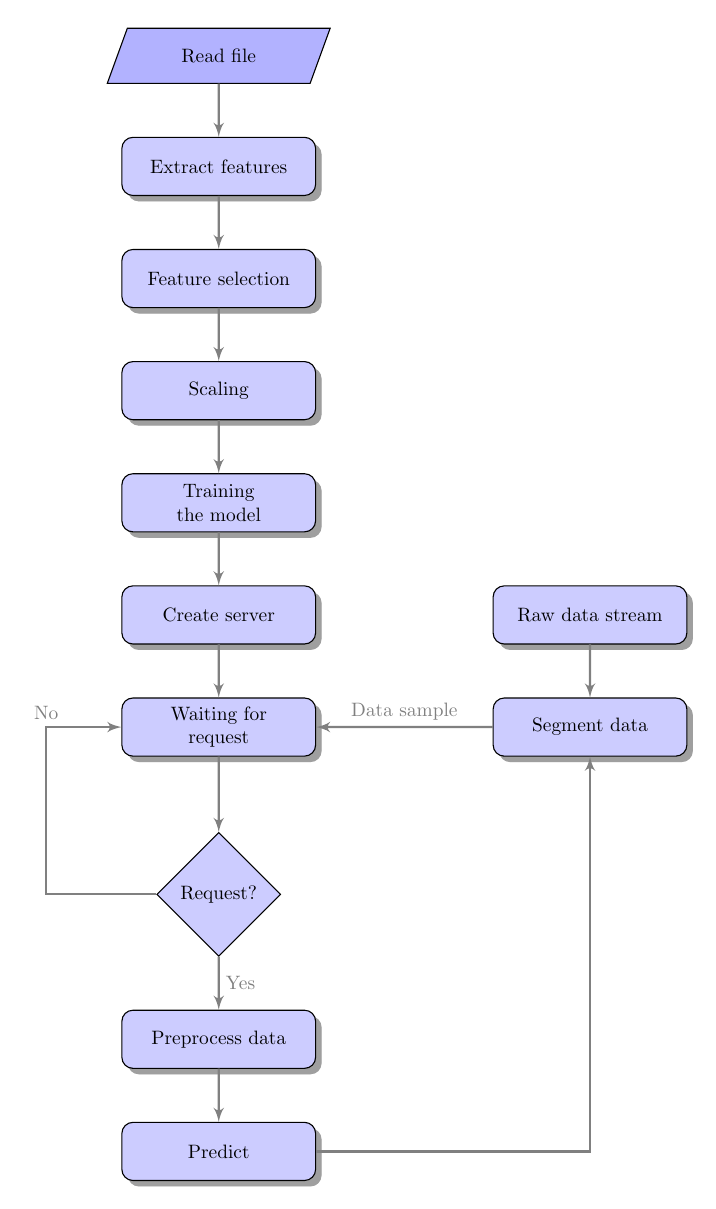
\begin{tikzpicture}[scale=0.7,transform shape]
	
	% Draw diagram elements
	%  \path \io{1}{Raw data};
	\path \io{1}{Read file};
	%  \path (p1.south)+(0,-1.5) \etape{2}{Extract steps};
	\path (p1.south)+(0.0,-1.5) \etape{2}{Extract features};
	\path (p2.south)+(0.0,-1.5) \etape{3}{Feature selection};
	
	\path (p3.south)+(0.0,-1.5) \etape{4}{Scaling};
	\path (p4.south)+(0.0,-1.5) \etape{12}{Training the model};
	
	\path (p12.south)+(0,-1.5) \etape{5}{Create server};
	\path (p5.south)+(0,-1.5) \etape{6}{Waiting for request};
	\path (p6.south)+(0,-2.5) \dec{7}{Request?};
	\path (p7.south)+(0,-1.5) \etape{8}{Preprocess data};
	\path (p8.south)+(0,-1.5) \etape{9}{Predict};
	
	
	%\path (request?.south)+(0,-1.5) \etape{7}{Predicted};
	
	\path (p5.west)+(8.5,0) \etape{10}{Raw data stream};
	\path (p10.south)+(0,-1.5) \etape{11}{Segment data};


	


	% Draw arrows between elements
	\path [line] (p1.south) -- node [above] {} (p2);
	\path [line] (p2.south) -- node [above] {} (p3);
	\path [line] (p3.south) -- node [above] {} (p4);
	\path [line] (p4.south) -- node [above] {} (p12);
	\path [line] (p12.south) -- node [above] {} (p5);
	\path [line] (p5.south) -- node [above] {} (p6);
	\path [line] (p6.south) -- node [above] {} (p7);
	\path [line] (p7.south) -- node [right] {Yes} (p8);
	\path [line] (p7.west) -- ++(-2,0) |- node [above] {No} (p6);
	\path [line] (p8.south) -- node [above] {} (p9);
	\path [line] (p9.east) -| node [above] {} (p11);
	
	\path [line] (p10.south) -- node [above] {} (p11);
	\path [line] (p11.west) -- node [above] {Data sample} (p6);
%	\path [line] (p11.south) -- node [above] {} (p4);

	
%	\path [line] (p5.south) -- node [above] {} (p6);

%	\path [line] (p4.south) -- node [right] {} (p9);

%	\path [line,dashed] (p6) -- node [above]{Data sample} (p9);
%	\path [line] (p9.south) -- node [right] {} (p7);
	
	\end{tikzpicture}
	
	\caption{The figure showing steps } \label{fig:M1}
\end{figure}
\FloatBarrier




\subsection{Floor to carpet}
The data is shown in figure \ref{fig:gulvet4teppegraf} and the table \ref{tab:Gulvet4teppe} show how the probability of each step. This experiment let the robot walk four step on floor and the rest on carpet. Even the overall accuracy in this test is approximately 88.9\%. However, for each step where it predicted correctly (marked green on \ref{tab:Gulvet4teppe}), is lower. For the first four step when it walked on the floor the probability is low. From fourth to fifth step is the crossing to new terrain. As it can be seen the probability is decreased. The fifth step is predicted is confused between carpet and floor. The rest has still a low probability of predicting correct.

\begin{figure}[h]
    \centering
    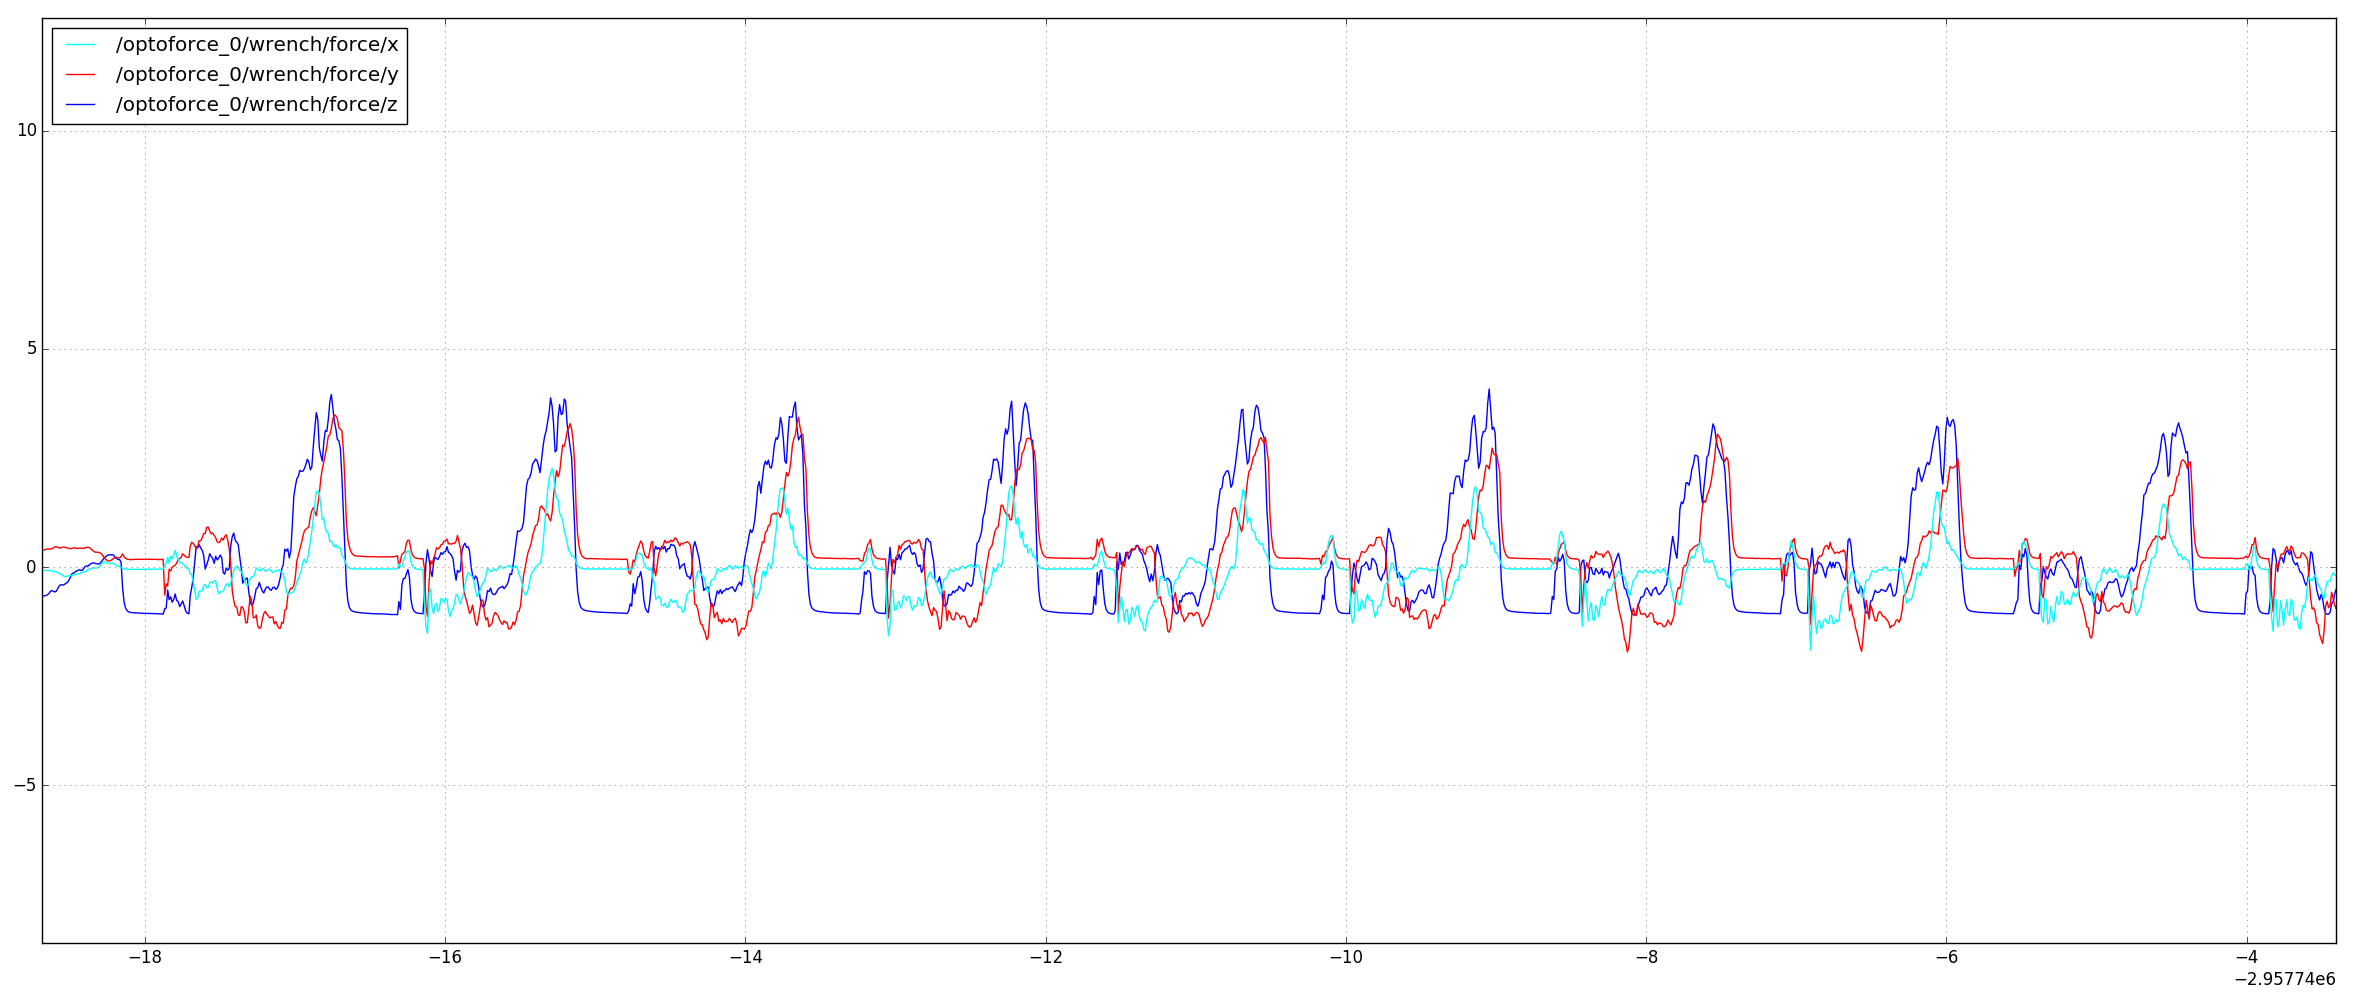
\includegraphics[width=\textwidth,height=\textheight,keepaspectratio]{Figures/Gulvet4Teppe2}
    \caption{Figure showing an the optofoce used in this thesis \cite{OptoforceFig}}
    \label{fig:gulvet4teppegraf}
\end{figure}


\begin{table}[h]
\centering
\resizebox{\textwidth}{!}{%
\begin{tabular}{@{}llllllllll@{}}
\toprule
\rowcolor[HTML]{FFFFC7} 
\textbf{Step} & \textbf{1} & \textbf{2} & \textbf{3} & \textbf{4} & \textbf{5} & \textbf{6} & \textbf{7} & \textbf{8} & \textbf{9} \\ \midrule
Floor & \cellcolor[HTML]{34FF34}0.782 & \cellcolor[HTML]{34FF34}0.680 & \cellcolor[HTML]{34FF34}0.747 & \cellcolor[HTML]{34FF34}0.561 & \cellcolor[HTML]{FD6864}0.564 & 0.282 & 0.206 & 0.252 & 0.282 \\
Carpet & 0.105 & 0.289 & 0.162 & 0.425 & \cellcolor[HTML]{F8FF00}0.353 & \cellcolor[HTML]{34FF34}0.704 & \cellcolor[HTML]{34FF34}0.730 & \cellcolor[HTML]{34FF34}0.573 & \cellcolor[HTML]{34FF34}0.599 \\
Soft mat & 0.008 & 0.009 & 0.010 & 0.008 & 0.010 & 0.005 & 0.009 & 0.009 & 0.015 \\
Hard mat & 0.104 & 0.022 & 0.081 & 0.007 & 0.073 & 0.010 & 0.055 & 0.166 & 0.104 \\ \bottomrule
\end{tabular}%
}
\caption{Gulvet4teppe}
\label{tab:Gulvet4teppe}
\end{table}
\FloatBarrier


\subsection{Hard mat to carpet}
The data is shown in figure \ref{fig:gulvet4teppegraf} and the table \ref{tab:Gulvet4teppe} show how the probability of each step. This experiment let the robot walk four step on floor and the rest on carpet. Even the overall accuracy in this test is approximately 88.9\%. However, for each step where it predicted correctly (marked green on \ref{tab:Gulvet4teppe}), is lower. For the first four step when it walked on the floor the probability is low. From fourth to fifth step is the crossing to new terrain. As it can be seen the probability is decreased. The fifth step is predicted is confused between carpet and floor. The rest has still a low probability of predicting correct.

\begin{figure}[h]
    \centering
    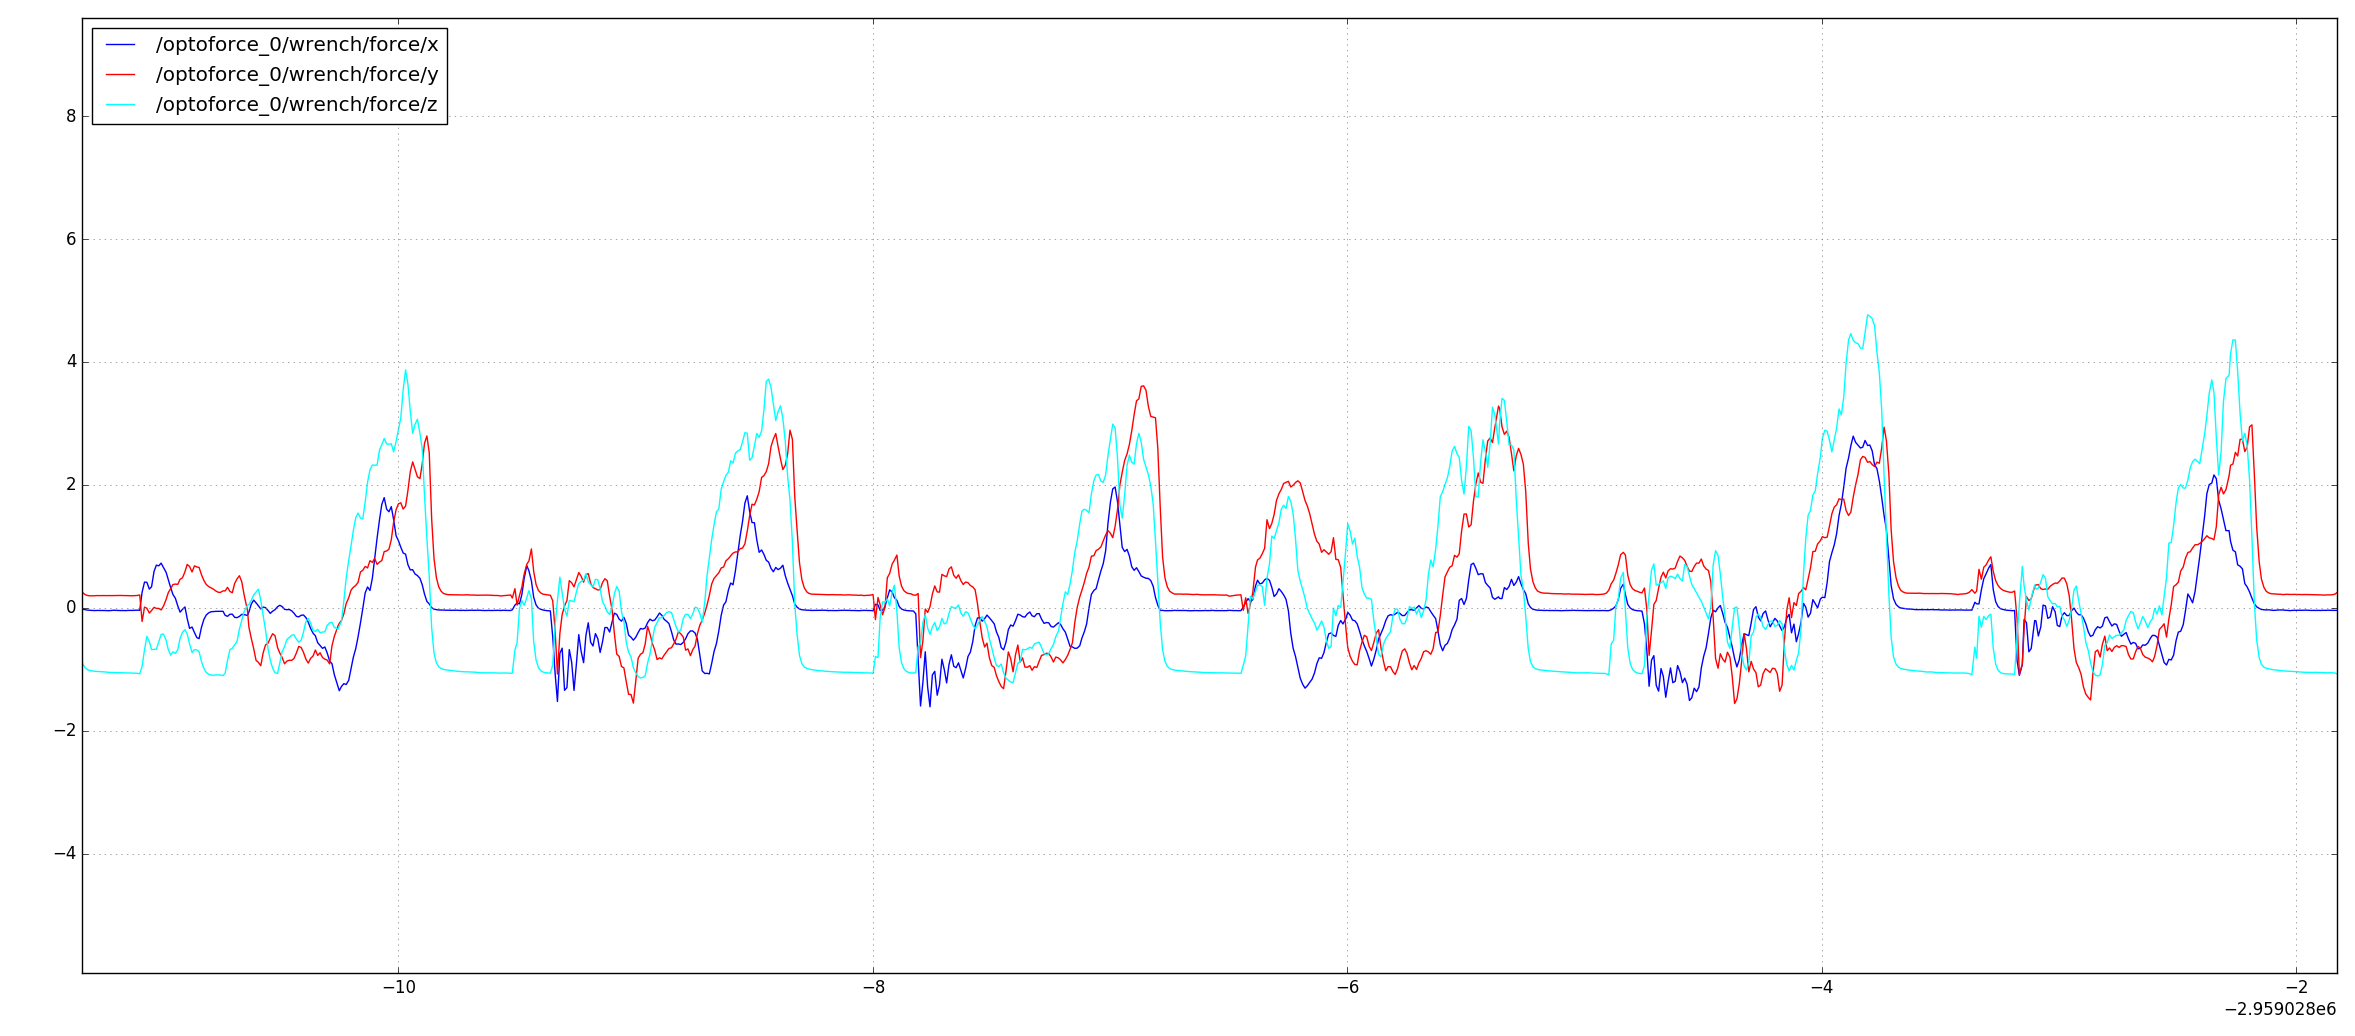
\includegraphics[width=\textwidth,height=\textheight,keepaspectratio]{Figures/MB3_3_Gulvet}
    \caption{Figure showing an the optofoce used in this thesis \cite{OptoforceFig}}
    \label{fig:optoforce}
\end{figure}
\begin{table}[h]
\centering
\resizebox{\textwidth}{!}{%
\begin{tabular}{@{}lllllll@{}}
\toprule
\rowcolor[HTML]{FFFFC7} 
\textbf{Step} & \textbf{1} & \textbf{2} & \textbf{3} & \textbf{4} & \textbf{5} & \textbf{6} \\ \midrule
Floor & 0.006 & 0.008 & 0.162 & 0.263 & 0.141 & 0.061 \\
Carpet & 0.008 & 0.113 & \cellcolor[HTML]{F8FF00}0.426 & \cellcolor[HTML]{34FF34}0.641 & \cellcolor[HTML]{34FF34}0.615 & \cellcolor[HTML]{34FF34}0.841 \\
Soft mat & 0.006 & 0.004 & 0.008 & 0.023 & 0.019 & 0.014 \\
Hard mat & \cellcolor[HTML]{34FF34}0.980 & \cellcolor[HTML]{34FF34}0.875 & \cellcolor[HTML]{FD6864}0.404 & 0.073 & 0.225 & 0.085 \\ \bottomrule
\end{tabular}%
}
\caption{Hard mat Teppe}
\label{my-label}
\end{table}


\begin{table}[h]
\centering
\resizebox{\textwidth}{!}{%
\begin{tabular}{@{}lllllll@{}}
\toprule
\rowcolor[HTML]{FFFFC7} 
\textbf{Step} & \textbf{1} & \textbf{2} & \textbf{3} & \textbf{4} & \textbf{5} & \textbf{6} \\ \midrule
Floor & 0.006 & 0.008 & \cellcolor[HTML]{F8FF00}0.162 & \cellcolor[HTML]{F8FF00}0.263 & \cellcolor[HTML]{F8FF00}0.141 & \cellcolor[HTML]{F8FF00}0.061 \\
Carpet & 0.008 & 0.113 & 0.426 & \cellcolor[HTML]{FD6864}0.641 & \cellcolor[HTML]{FD6864}0.615 & \cellcolor[HTML]{FD6864}0.841 \\
Soft mat & 0.006 & 0.004 & 0.008 & 0.023 & 0.019 & 0.014 \\
Hard mat & \cellcolor[HTML]{34FF34}0.980 & \cellcolor[HTML]{34FF34}0.875 & \cellcolor[HTML]{FD6864}0.404 & 0.073 & 0.225 & 0.085 \\ \bottomrule
\end{tabular}%
}
\caption{Hard mat eller gulv}
\label{my-label}
\end{table}

\FloatBarrier

\subsection{Hard mat to soft mat}
The data is shown in figure \ref{fig:hardmatSoftMat} and the table \ref{hardmatSoftMat} show how the probability of each step in transition from hard mat to soft mat. The overall performance is 100\% accurate, while the mean of correct predicted is approximately 72\%. 

\begin{figure}[h]
    \centering
    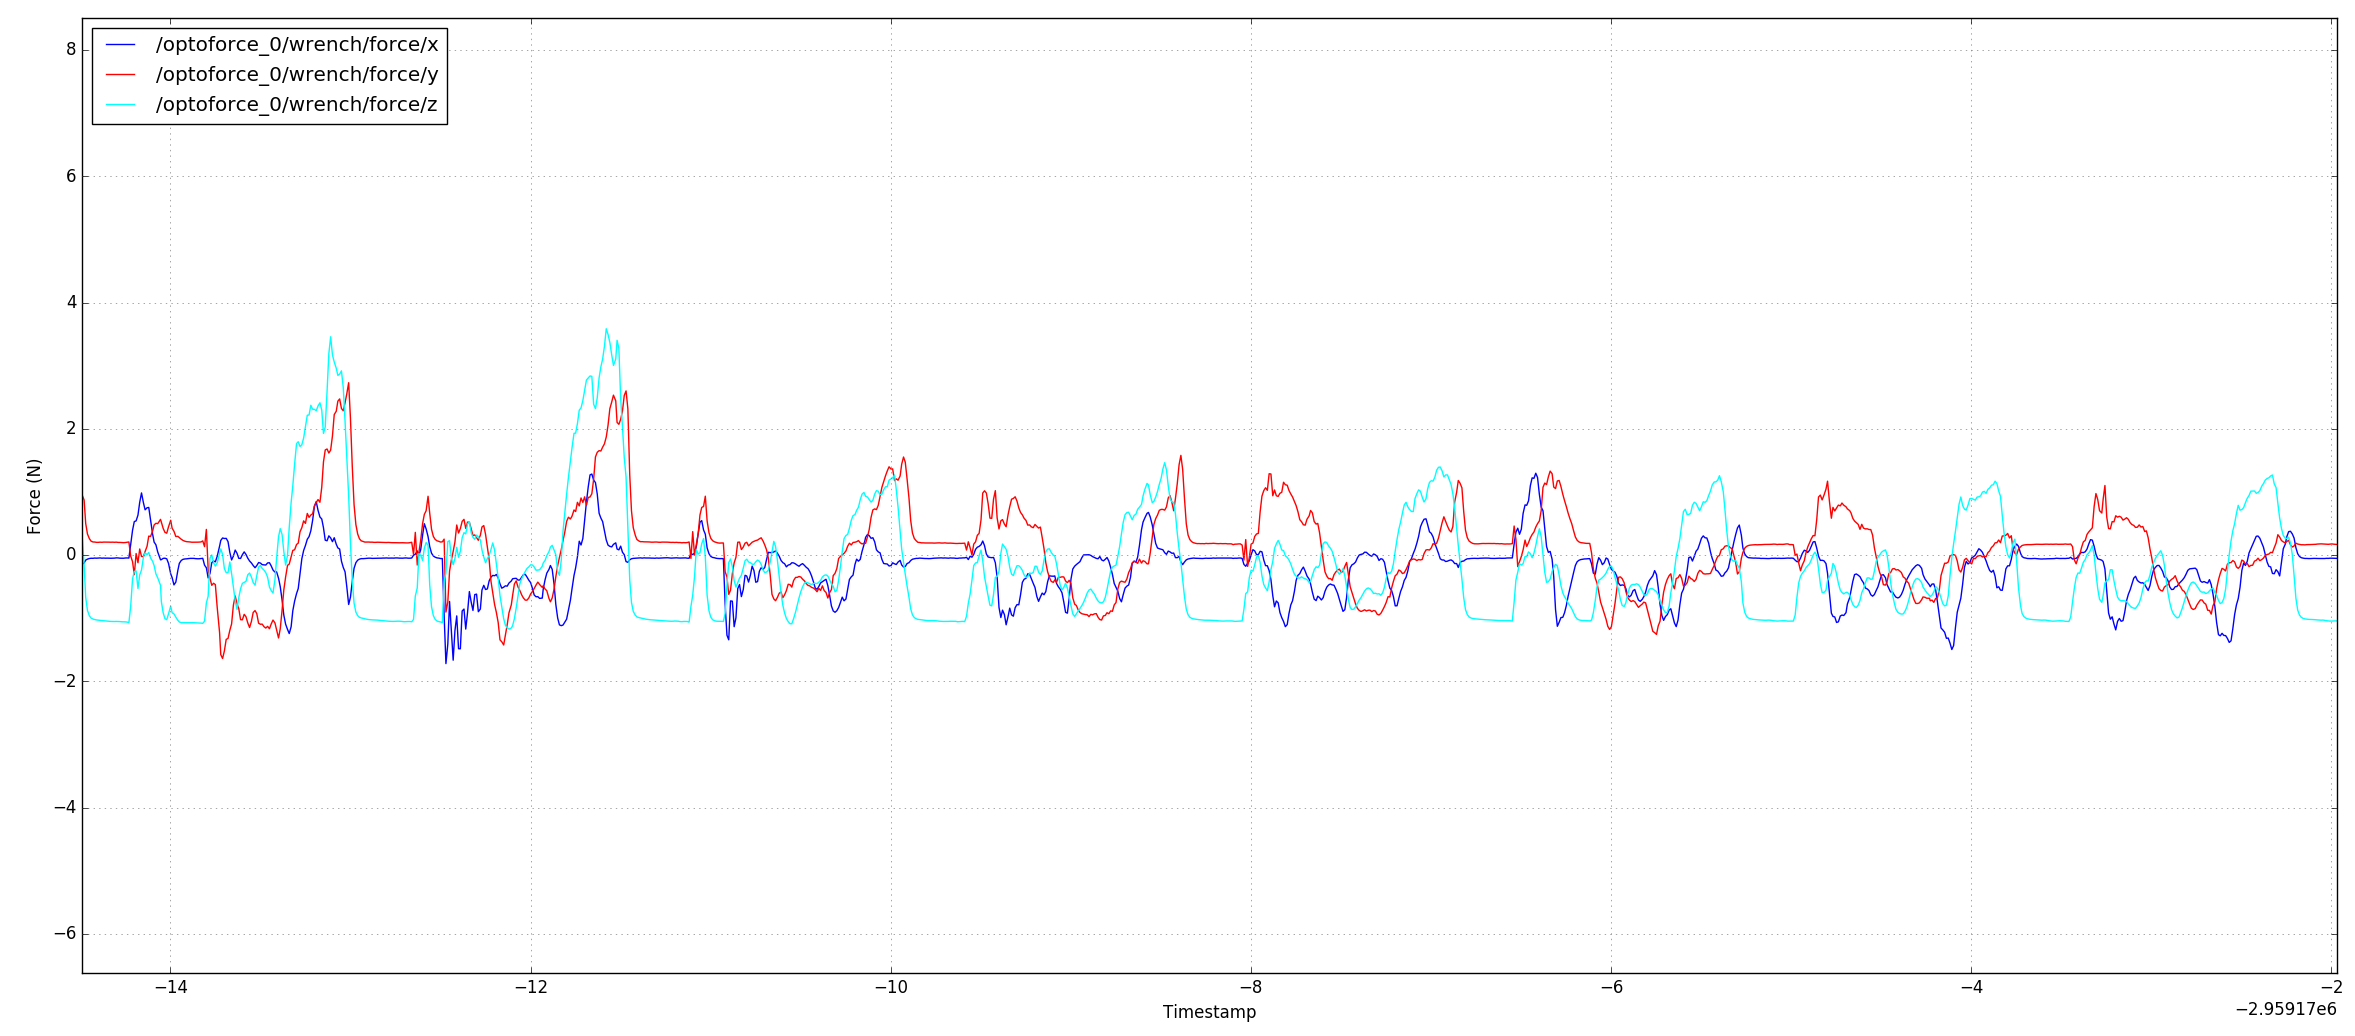
\includegraphics[width=\textwidth,height=\textheight,keepaspectratio]{Figures/MB3MM}
    \caption{Figure showing an the optofoce used in this thesis \cite{OptoforceFig}}
    \label{fig:hardmatSoftMat}
\end{figure}

\begin{table}[h]
\centering
\resizebox{\textwidth}{!}{%
\begin{tabular}{@{}lllllllll@{}}
\toprule
\rowcolor[HTML]{FFFFC7} 
\textbf{Step} & \textbf{1} & \textbf{2} & \textbf{3} & \textbf{4} & \textbf{5} & \textbf{6} & 7 & 8 \\ \midrule
Floor & 0.329 & 0.015 & 0.081 & 0.059 & 0.022 & 0.115 & 0.059 & 0.048 \\
Carpet & 0.105 & 0.045 & 0.105 & 0.041 & 0.015 & 0.095 & 0.037 & 0.033 \\
Soft mat & 0.023 & 0.006 & 0.284 & \cellcolor[HTML]{34FF34}0.759 & \cellcolor[HTML]{34FF34}0.923 & \cellcolor[HTML]{34FF34}0.477 & \cellcolor[HTML]{34FF34}0.816 & \cellcolor[HTML]{34FF34}0.834 \\
Hard mat & \cellcolor[HTML]{34FF34}0.542 & \cellcolor[HTML]{34FF34}0.935 & \cellcolor[HTML]{34FF34}0.529 & 0.142 & 0.040 & 0.313 & 0.088 & 0.085 \\ \bottomrule
\end{tabular}%
}
\caption{Hard matte 3 myk matte}
\label{hardmatSoftMat}
\end{table}
\FloatBarrier

\subsection{Soft mat to hard mat}
The data is shown in figure \ref{fig:MM_4_Resten_BGraf} and the table \ref{MM4MB} show how the probability of each step. This experiment let the robot walk four step on floor and the rest on carpet. Even the overall accuracy in this test is approximately 100\%. The first step and the transistion step has the lowest probability it maight indicate that the data differ. It also can be seen that at the fourth step there is. Except for that the overall is high probability of predicting correct. 

\begin{figure}[h]
    \centering
    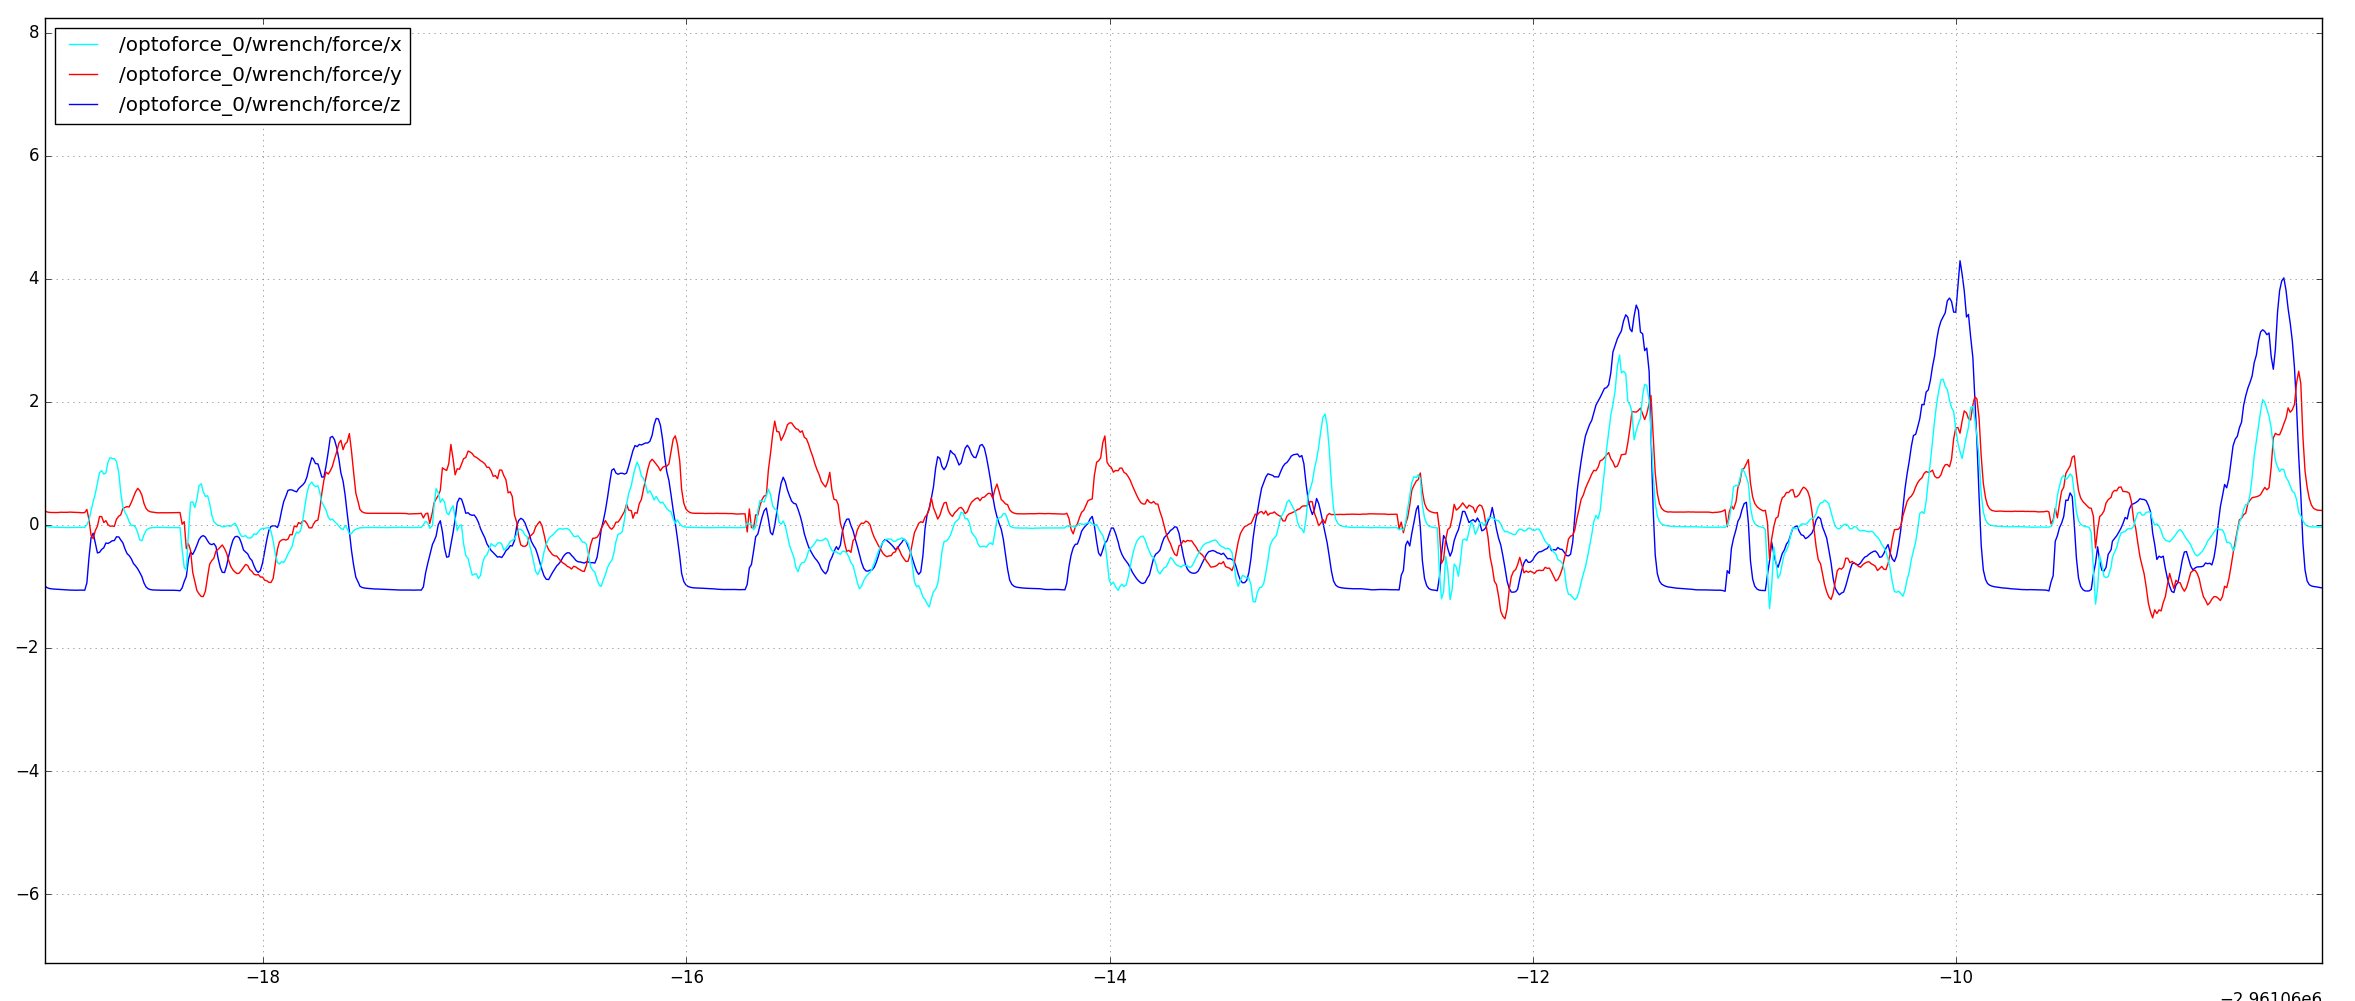
\includegraphics[width=\textwidth,height=\textheight,keepaspectratio]{Figures/MM_4Resten_MB}
    \caption{Figure showing an the optoforce used in this thesis \cite{OptoforceFig}}
    \label{fig:MM_4_Resten_BGraf}
\end{figure}

\begin{table}[h]
\centering
\resizebox{\textwidth}{!}{%
\begin{tabular}{@{}llllllll@{}}
\toprule
\rowcolor[HTML]{FFFFC7} 
\textbf{Step} & \textbf{1} & \textbf{2} & \textbf{3} & \textbf{4} & \textbf{5} & \textbf{6} & 7 \\ \midrule
Floor & 0.099 & 0.019 & 0.018 & 0.138 & 0.021 & 0.008 & 0.038 \\
Carpet & 0.065 & 0.023 & 0.017 & 0.134 & 0.050 & 0.005 & 0.022 \\
Soft mat & \cellcolor[HTML]{34FF34}0.535 & \cellcolor[HTML]{34FF34}0.871 & \cellcolor[HTML]{34FF34}0.911 & \cellcolor[HTML]{34FF34}0.384 & 0.009 & 0.009 & 0.011 \\
Hard mat & 0.300 & 0.086 & 0.054 & 0.344 & \cellcolor[HTML]{34FF34}0.921 & \cellcolor[HTML]{34FF34}0.978 & \cellcolor[HTML]{34FF34}0.930 \\ \bottomrule
\end{tabular}%
}
\caption{MM 4Resten MBNY}
\label{MM4MB}
\end{table}
\FloatBarrier
\subsection{Soft mat to carpet}
The data is shown in figure \ref{fig:MM_4_Resten_BGraf} and the table \ref{MM4MB} show how the probability of each step. This experiment let the robot walk four step on floor and the rest on carpet. It predicted 7/8 correct. As seen in the figure \ref{MM4MB}, there is a large variation from walking soft mat to carpet. On small soft mat the amplitude is significant smaller than carpet. At the step five, the probability of carpet is approximately 66.7\%, the number might seems low, but the other is significant lower which make it no confusion. Regarding step six, where it wrong prediction between carpet and hard mat. There is a high probability of hard hard mat. A few factors which might cause that, is looking to the figure \ref{fig:MM_4_Resten_BGraf}. The shape y direction differ from the other, and so do the amplitude too.


\begin{figure}[h]
    \centering
    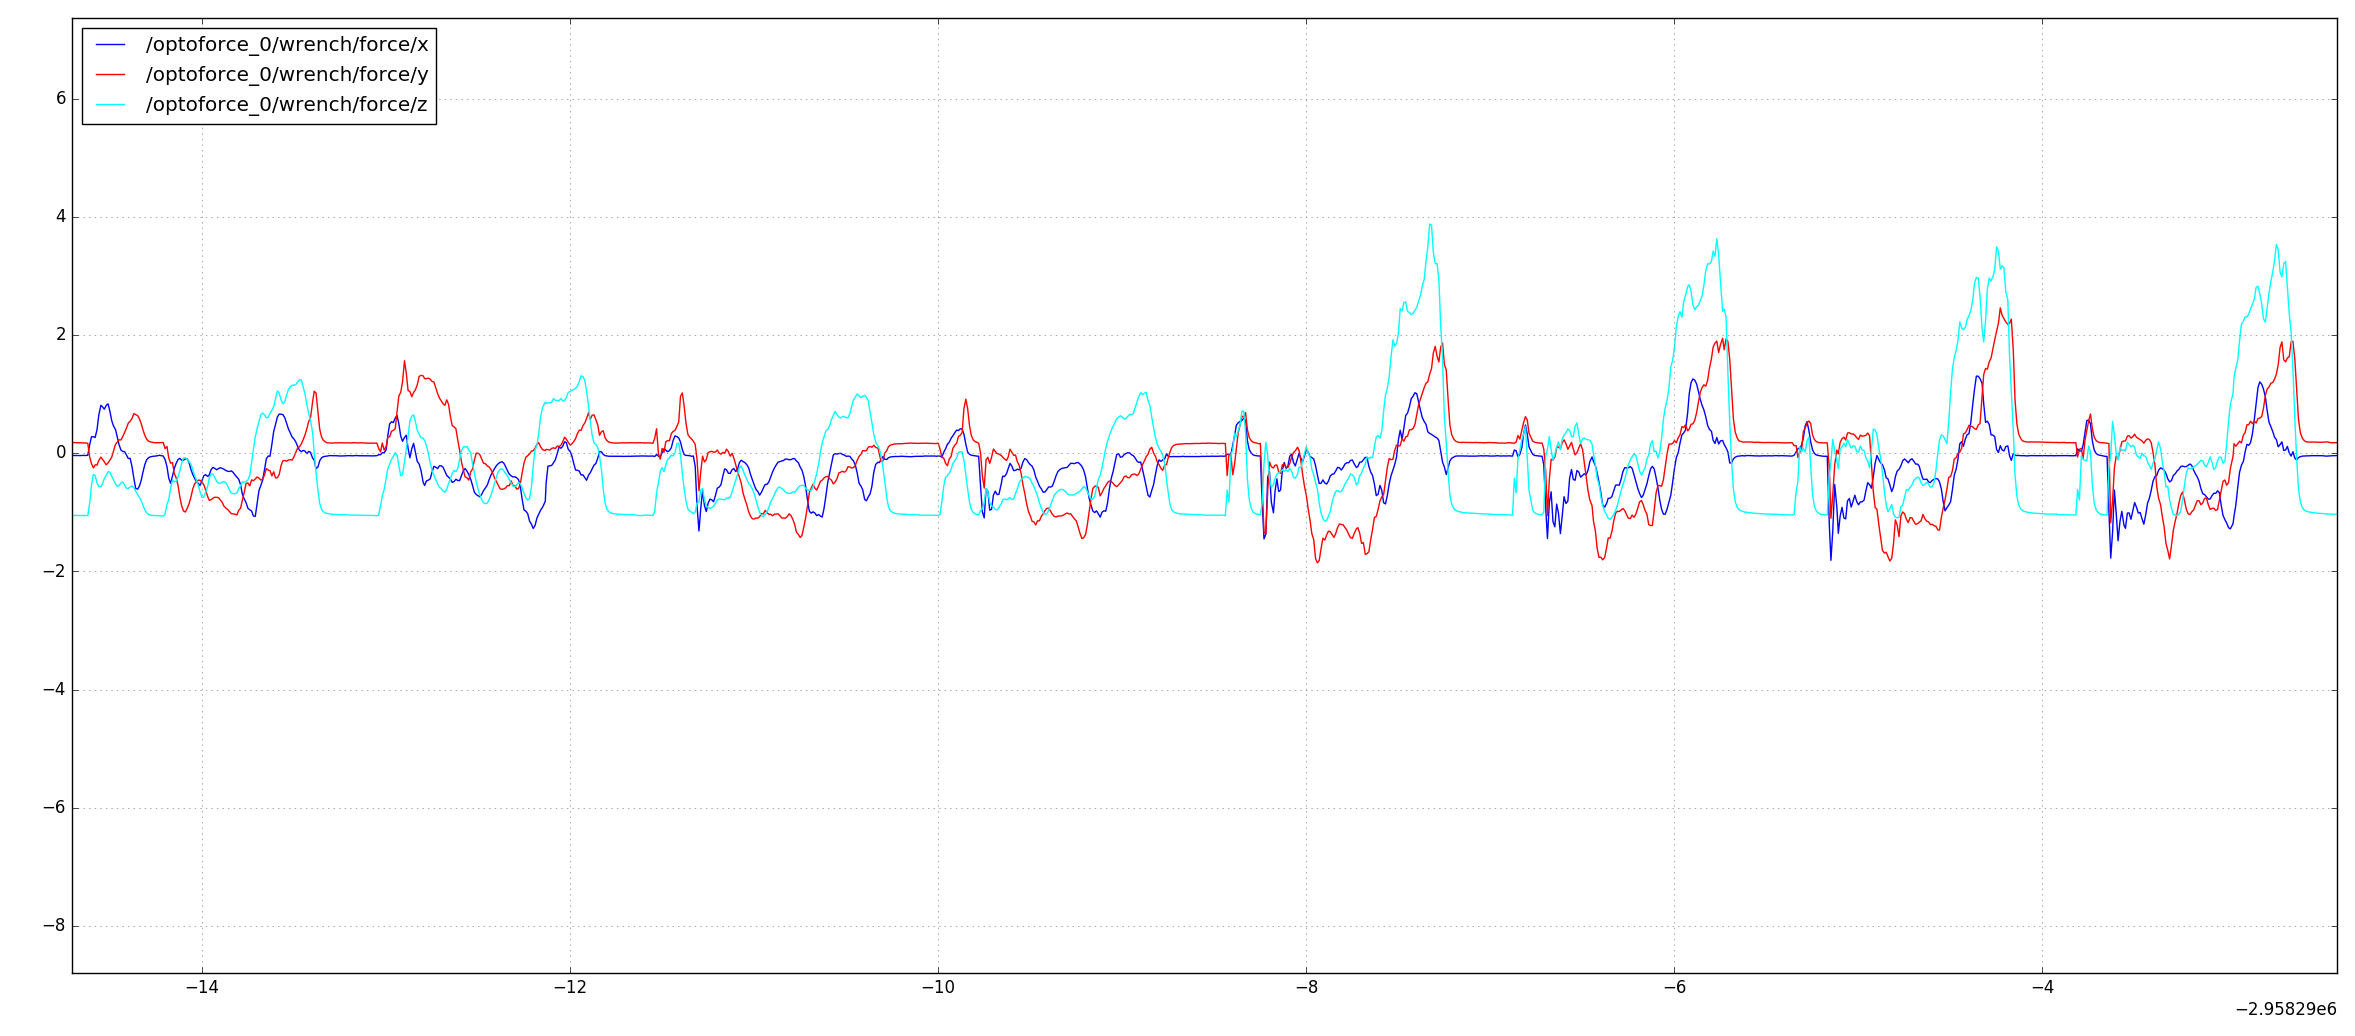
\includegraphics[width=\textwidth,height=\textheight,keepaspectratio]{Figures/MM4Teppe2}
    \caption{Figure showing an the optofoce used in this thesis \cite{OptoforceFig}}
    \label{fig:optoforce}
\end{figure}

\begin{table}[h]
\centering
\resizebox{\textwidth}{!}{%
\begin{tabular}{@{}lllllllll@{}}
\toprule
\rowcolor[HTML]{FFFFC7} 
\textbf{Step} & \textbf{1} & \textbf{2} & \textbf{3} & \textbf{4} & \textbf{5} & \textbf{6} & 7 & 8 \\ \midrule
Floor & 0.021 & 0.022 & 0.068 & 0.031 & 0.100 & 0.020 & 0.016 & 0.018 \\
Carpet & 0.017 & 0.019 & 0.049 & 0.023 & \cellcolor[HTML]{34FF34}0.667 & \cellcolor[HTML]{F8FF00}0.041 & \cellcolor[HTML]{34FF34}0.942 & \cellcolor[HTML]{34FF34}0.904 \\
Soft mat & \cellcolor[HTML]{34FF34}0.909 & \cellcolor[HTML]{34FF34}0.914 & \cellcolor[HTML]{34FF34}0.762 & \cellcolor[HTML]{34FF34}0.891 & 0.017 & 0.007 & 0.006 & 0.006 \\
Hard mat & 0.054 & 0.045 & 0.121 & 0.055 & 0.216 & \cellcolor[HTML]{FD6864}0.933 & 0.037 & 0.072 \\ \bottomrule
\end{tabular}%
}
\caption{MM4 Teppe}
\label{my-label}
\end{table}
\FloatBarrier
\subsection{Summary}
It is shown that the probability at transistion is typcially low value. The might indicate that the sensor is sensitive. The training samples only trained with one each terrain, which may be better to train differently. Is also seen that in the beginning the probability of correct terrain is also typically low. It might indicate that the first step is strange, as the in the middle the robot got more stable, thus more training data and more accurately. It is shown that the sensor is capable to distinguish minor differently terrain, even the probability is low. Soft mat has a low start.

\section{Prediction next sensor?}




\chapter{Conclusion}



\subsection{Future work}
Improvment of classifier
The classifier is based on the features of the robot motion and interaction with the terrain. However, the features of the terrain itself such as slopiness, slipperiness, convexity, hardness, are not analyzed directly - they may be hidden inside the classifier and could be addressed in the future work.

Other classifier, other features extraction.

The learning is based on each step, maybe collect data from more than one step.

Rely only on optoforce sensor, other sensor such as servo, knee etc....

Teste om the holder å se på en retning?

Ikke decimate - kan miste viktige features

Oter experiments
To og to bein på forskjellige underlag

Trening på forskjellige overgang
http://www2.ift.ulaval.ca/~pgiguere/terrainID.html

%Optical force (Legged Robots)
%https://link.springer.com/referenceworkentry/10.1007/978-3-540-30301-5_17

An Overview of Legged Robots

\backmatter{}
\bibliography{bib}
\bibliographystyle{ieeetr}
\end{document}
